\documentclass[11pt,a4paper]{article}

\usepackage[T1]{fontenc}
\usepackage[utf8]{inputenc}
\usepackage[sc]{mathpazo}
\linespread{1.04}
\usepackage[scaled=0.86]{helvet}
\usepackage[margin=1in]{geometry}
\usepackage{amsmath,amssymb,amsthm,mathtools}
\usepackage{booktabs}
\usepackage{array}
\usepackage{tabularx}
\usepackage{float}
\usepackage[hidelinks]{hyperref}
\usepackage[nameinlink,noabbrev]{cleveref}
\usepackage{microtype}
\usepackage{enumitem}
\usepackage{siunitx}
\usepackage{xcolor}
\usepackage{caption}
\usepackage{tcolorbox}
\tcbuselibrary{skins,breakable}
\usepackage{thmtools}
\usepackage{tikz}
\usetikzlibrary{arrows.meta,positioning,calc,fit,backgrounds,matrix,decorations.pathmorphing}
\usepackage{pgfplots}
\pgfplotsset{compat=1.18}
\usepackage{longtable}
\usepackage{multirow}
\usepackage{makecell}
\usepackage{bm}
\usepackage{csquotes}
\usepackage{fancyhdr}
\usepackage{titlesec}

% ── Color palette ──
\definecolor{tfptblue}{RGB}{35,60,120}
\definecolor{tfptorange}{RGB}{190,100,20}
\definecolor{tfptgreen}{RGB}{40,110,60}
\definecolor{tfptgray}{RGB}{90,90,95}

\hypersetup{
    colorlinks=true,
    linkcolor=tfptblue!80!black,
    citecolor=tfptblue!70!black,
    urlcolor=tfptblue!60!black,
}

% ── Caption styling ──
\captionsetup{
    font={small,sf},
    labelfont={bf,color=tfptgray},
    labelsep=period,
    margin=1.5em,
    skip=6pt,
}

% ── Section heading styling ──
\titleformat{\section}
    {\Large\bfseries\color{tfptblue}}{\thesection}{0.8em}{}
\titleformat{\subsection}
    {\large\bfseries\color{tfptblue!85!black}}{\thesubsection}{0.7em}{}
\titleformat{\subsubsection}
    {\normalsize\bfseries\color{tfptblue!70!black}}{\thesubsubsection}{0.6em}{}
\titlespacing*{\section}{0pt}{1.8ex plus 0.6ex minus 0.3ex}{0.9ex plus 0.2ex}
\titlespacing*{\subsection}{0pt}{1.4ex plus 0.4ex minus 0.2ex}{0.6ex plus 0.1ex}

% ── Running headers ──
\pagestyle{fancy}
\fancyhf{}
\fancyhead[L]{\small\itshape\color{tfptgray} TFPT: Carrier Algebra, Closure Theorems, and Intrinsic Observation}
\fancyhead[R]{\small\color{tfptgray}\thepage}
\renewcommand{\headrulewidth}{0.4pt}
\renewcommand{\headrule}{\hbox to\headwidth{\color{tfptblue!30}\leaders\hrule height \headrulewidth\hfill}}
\fancypagestyle{plain}{\fancyhf{}\fancyfoot[C]{\small\color{tfptgray}\thepage}\renewcommand{\headrulewidth}{0pt}}

% ── tcolorbox global defaults ──
\tcbset{
    enhanced,
    boxrule=0.6pt,
    arc=2.5pt,
    left=6pt, right=6pt, top=5pt, bottom=5pt,
    fonttitle=\bfseries\sffamily\small,
    coltitle=white,
    toptitle=2pt, bottomtitle=2pt,
    shadow={0.8mm}{-0.6mm}{0mm}{black!12},
}

\sisetup{
    detect-all,
    round-mode = none,
    exponent-mode = input,
    exponent-product = \times,
    group-separator = {\,},
    group-minimum-digits = 4
}

\newtheorem{theorem}{Theorem}[section]
\newtheorem{corollary}[theorem]{Corollary}
\newtheorem{lemma}[theorem]{Lemma}
\theoremstyle{definition}
\newtheorem{definition}[theorem]{Definition}
\newtheorem{conjecture}[theorem]{Conjecture}
\newtheorem{proposition}[theorem]{Proposition}
\newtheorem{assumption}[theorem]{Assumption}
\newtheorem{principle}[theorem]{Principle}
\newtheorem{construction}[theorem]{Construction}
\newtheorem{claim}[theorem]{Claim}
\newtheorem{appendixstep}[theorem]{Appendix Step}
\theoremstyle{remark}
\newtheorem*{remark}{Remark}

\makeatletter
\def\theHtheorem{\thesection.\thetheorem}
\def\theHcorollary{\theHtheorem}
\def\theHlemma{\theHtheorem}
\def\theHdefinition{\theHtheorem}
\def\theHconjecture{\theHtheorem}
\def\theHproposition{\theHtheorem}
\def\theHassumption{\theHtheorem}
\def\theHprinciple{\theHtheorem}
\def\theHconstruction{\theHtheorem}
\def\theHclaim{\theHtheorem}
\def\theHappendixstep{\theHtheorem}
\makeatother

\DeclareMathOperator{\tr}{Tr}
\DeclareMathOperator{\rank}{rank}
\DeclareMathOperator{\SF}{SF}
\DeclareMathOperator{\Ind}{Ind}
\DeclareMathOperator{\argmin}{arg\,min}

\newcolumntype{Y}{>{\raggedright\arraybackslash}X}

\newcommand{\Seam}{\Sigma}
\newcommand{\inv}{\iota}
\newcommand{\Mpl}{\bar M_{\mathrm{Pl}}}
\newcommand{\Mplunred}{M_{\mathrm{Pl}}}
\newcommand{\cthree}{c_3}
\newcommand{\atheta}{a_\theta}
\newcommand{\phibase}{\varphi_{\mathrm{base}}}
\newcommand{\phiz}{\varphi_0^{\mathrm{ret}}}
\newcommand{\phiseam}{\varphi_{\Sigma}}
\newcommand{\deltatop}{\delta_{\mathrm{top}}}
\newcommand{\bone}{b_1}
\newcommand{\SM}{\mathrm{SM}}
\newcommand{\QCD}{\mathrm{QCD}}
\newcommand{\Oadm}{\Omega_{\mathrm{adm}}}
\newcommand{\Cmin}{\mathcal C_{\min}}
\newcommand{\Ageom}{\mathcal A_{\mathrm{geom}}}
\newcommand{\Atrans}{\mathcal A_{\mathrm{trans}}}
\newcommand{\Arec}{\mathcal A_{\mathrm{rec}}}
\newcommand{\Aobs}{\mathcal A_{\mathrm{obs}}}
\newcommand{\Asing}{\mathcal A_{\mathrm{sing}}}
\newcommand{\Vadm}{\mathcal V_{\mathrm{adm}}}
\newcommand{\Hrel}{\mathcal H_{\mathrm{rel}}}
\newcommand{\Hhad}{\mathcal H_{\mathrm{had}}}
\newcommand{\Hhub}{H_{\mathrm{hub}}}
\newcommand{\Htot}{\mathcal H_{\mathrm{tot}}}
\newcommand{\Gammaeff}{\Gamma_{\mathrm{eff}}}
\newcommand{\lambdaY}{\lambda_Y}
\newcommand{\Pred}{\operatorname{Pred}}
\newcommand{\gcar}{g_{\mathrm{car}}}
\newcommand{\Hint}{\mathcal H_{\mathrm{int}}}
\newcommand{\Kadm}{K_{\mathrm{adm}}}
\newcommand{\Tmin}{\mathfrak T_{\mathrm{min}}}
\newcommand{\Tprim}{\mathfrak T_{\mathrm{prim}}}
\newcommand{\chiseed}{\chi_{\mathrm{seed}}}
\newcommand{\chigeo}{\chi_{\mathrm{geo}}}
\newcommand{\chigeozero}{\chi_{\mathrm{geo},0}}
\newcommand{\APSdom}{\mathrm{APS}_{\mathrm{dom}}}
\newcommand{\APSfam}{\mathrm{APS}_{\mathrm{fam}}}
\newcommand{\vgeo}{v_{\mathrm{geo}}}
\newcommand{\vewref}{v_{\mathrm{EW}}^{\mathrm{ref}}}
\newcommand{\Dstart}{D_{\mathrm{start}}}
\newcommand{\Tcore}{\mathfrak T_{\mathrm{core}}}
\newcommand{\Tbridge}{\mathfrak T_{\mathrm{bridge}}}
\newcommand{\Tker}{\mathfrak T_{\mathrm{ker}}}
\newcommand{\Tcomp}{\mathfrak T_{\mathrm{comp}}}
\newcommand{\Padm}{P_{\mathrm{adm}}}
\newcommand{\wspin}{\varpi_{\mathrm{spin}}}

\title{%
    \color{tfptblue}\textbf{TFPT: Carrier Algebra, Closure Theorems,\\and Intrinsic Observation}\\[0.6em]
    {\Large\color{tfptgray} An overdetermined rank-5 spectral theory\\from the admissible reduced datum}
}
\author{Stefan Hamann \and Alessandro Rizzo}
\date{{\normalsize\color{tfptgray}\sffamily Version 4.1\enspace--\enspace Generative Closure\enspace--\enspace\today}}

\begin{document}
\maketitle

\begin{abstract}
From the admissible reduced datum
\[
\Tmin^{\mathrm{adm}}=(\mathcal A,\mathcal H,D,J,\Gamma,\inv,\nu),
\]
the carrier-first architecture reconstructs the primitive layer, the unique minimal carrier
$E_3\oplus E_2$, the global Standard Model quotient
$S(U(3)\times U(2))\cong(SU(3)\times SU(2)\times U(1)_Y)/\mathbb Z_6$, one chiral family
with $\nu^c$ from the positive half-spinor, the hypercharge--seam inversion
$6Y^2-Y-\mathbf 1=0$, and the exact electromagnetic closure equation whose canonical
admissible branch reproduces $\alpha^{-1}(0)=\num{137.0359992}$.

The same theorem surface then generates the canonical two-stage admissibility selector
\[
\Padm=P_{\mathrm{str}}P_{\mathrm{gap}},
\qquad
P_{\mathrm{str}}:=P_{\Seam,+}P_{\mathrm{sing}}P_\Theta,
\]
the topological family closure $F\cong\mathbb C^3$ and $\Oadm=48$, and a conditional
geometric reconstruction in which the Dirac anchor
\[
D_{\mathrm{geo}}:=D_{\mathrm{ref}}+D_{\mathrm{rel}}=D
\]
carries the metric, spin, and local spectral-scale data while the admissible compression
governs retained observables. The transport sector is organized on a canonical numerically
selected admissible branch with exact Yukawa formulas, hadronic singlet selection,
strong-CP protection, reflection positivity, and Lorentzian reconstruction.

The observation layer is formulated as a conditional closure selection theorem: once
coercivity and local Hessian positivity hold on the admissible domain, selected minimizers
are read by the observation functor $\mathcal R_{\mathrm{TOE}}$. Matched benchmark ledgers
are reported on the canonical selected branch, while optional downstream modules evaluate
UV Bernstein-cone and cosmology-facing quantities from the same retained operator data.

Compression identities remain structural rather than decorative: once the optional occupancy
compression is imposed, the rank-lock $2^{g-3}=g-1$ fixes $g=5$, the hard $41$-chain
$10\,b_1=\Omega_{\mathrm{adm}}\gamma+1=41$ overdetermines the canonical branch, and wrong
discrete worlds still fail the electromagnetic closure decisively. Optional E$_8$
arithmetic continuations, asymptotic expansions, and horizon language are retained only as
appendix-level extrapolations and are not part of the closed theorem surface.
\end{abstract}

\begin{tcolorbox}[colback=tfptblue!2, colframe=tfptblue!40, breakable,
    title={Reading Status for the Present Paper}, colbacktitle=tfptblue!60]
\begin{itemize}[leftmargin=1.5em, topsep=3pt, itemsep=3pt]
    \item \textbf{Reduced datum:} $\Tmin^{\mathrm{adm}}=(\mathcal A,\mathcal H,D,J,\Gamma,\inv,\nu)$ with admissible spectral regularity, seam collar, and positive spectral measure.
    \item \textbf{Status classes:} exact algebraic, conditional geometric or closure, matched intrinsic observation, and optional extrapolation.
    \item \textbf{Exact algebraic layer:} primitive scaffold, minimal carrier $E_3\oplus E_2$, one-family packet, carrier constants, and exact electromagnetic closure.
    \item \textbf{Conditional geometric or closure layer:} two-stage admissibility selector, topological family closure, Dirac-anchor geometry, transport-branch program, hadronic and strong-CP closure, Lorentz reconstruction, and the conditional UV Bernstein-cone program.
    \item \textbf{Matched intrinsic observation layer:} selected-branch ledgers, threshold rows, and the observation functor $\mathcal R_{\mathrm{TOE}}$.
    \item \textbf{Optional downstream modules:} cosmology-facing evaluations, E$_8$ scale grammar, asymptotic expansions, and horizon semantics.
\end{itemize}
\end{tcolorbox}

\tableofcontents

\section{Reading guide and claim map}

The paper is organized in three reading layers:
\begin{itemize}[leftmargin=1.5em, topsep=3pt, itemsep=2pt]
    \item \textbf{Big picture:} one section explains what TFPT claims in plain language before the detailed datum and conventions begin.
    \item \textbf{Detail:} the main body then runs from primitive core and hard carrier kernel through kernel numerics, the two closure-architecture sections, the closure theorem stack, the particle/mass compiler, and the benchmark interface.
    \item \textbf{Proof sketches:} the main text gives only the central proof sketches, while dense technical derivations remain in appendices or companion material.
\end{itemize}
The status language is also fixed once and for all:
\begin{itemize}[leftmargin=1.5em, topsep=3pt, itemsep=2pt]
    \item \textbf{Reduced datum} means the admissible spectral starting package from which the primitive scaffold is reconstructed.
    \item \textbf{Exact algebraic} means exact consequences of the carrier algebra, parity code, weight enumerator, and compression identities.
    \item \textbf{Conditional geometric or closure} means statements that depend on the geometric anchor, admissibility closure, APS input, positivity input, or selected retained branch.
    \item \textbf{Matched intrinsic observation} means rows read through the observation functor and benchmark map, including threshold outputs and convention-dependent comparisons.
    \item \textbf{Optional extrapolation} means appendix-level continuations not needed for the core.
\end{itemize}
To keep theorem language, benchmark semantics, and appendix bookkeeping lexically stable, all prose, captions, and status labels are kept in English throughout.

\begin{tcolorbox}[colback=tfptblue!2, colframe=tfptblue!40, breakable,
    title={Datum Hierarchy for the Present Draft}, colbacktitle=tfptblue!60]
\begin{itemize}[leftmargin=1.5em, topsep=3pt, itemsep=3pt]
    \item \textbf{Reduced datum:} $\Tmin^{\mathrm{adm}}$ with admissible center, involution, seam collar, and positive spectral measure.
    \item \textbf{Exact algebraic layer:} reconstructed primitive scaffold, minimal carrier $E_3\oplus E_2$, global quotient, one-family packet, and exact electromagnetic closure.
    \item \textbf{Conditional geometric or closure layer:} $\Padm$, topological family closure, Dirac-anchor geometry, Higgs selection, transport-branch program, hadronic sector, and conditional UV closure.
    \item \textbf{Matched intrinsic observation layer:} selected-branch thresholds, ledgers, and observable generation through $\mathcal R_{\mathrm{TOE}}$.
    \item \textbf{Optional extrapolation:} cosmology-facing modules, E$_8$ continuations, asymptotic transport expansions, and horizon semantics.
\end{itemize}
\end{tcolorbox}

\begin{figure}[t]
\centering
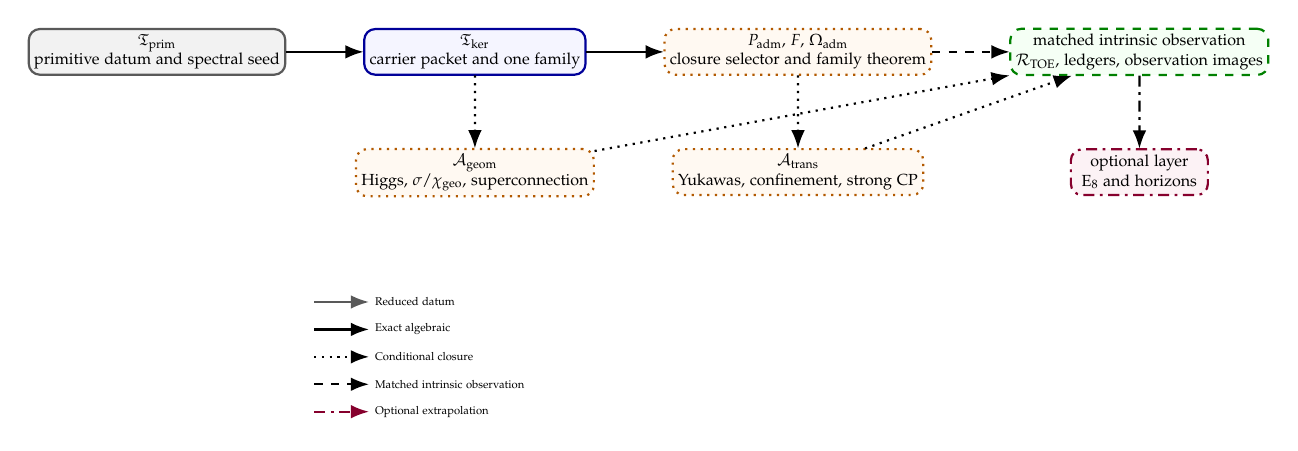
\begin{tikzpicture}[
    scale=0.58,
    transform shape,
    >=Latex,
    node distance=1.6cm and 1.7cm,
    primitive/.style={draw=gray!70!black, thick, rounded corners, fill=gray!10, align=center, minimum width=2.8cm, minimum height=1cm},
    hard/.style={draw=blue!60!black, thick, rounded corners, fill=blue!4, align=center, minimum width=2.8cm, minimum height=1cm},
    bridge/.style={draw=green!50!black, dashed, thick, rounded corners, fill=green!4, align=center, minimum width=2.9cm, minimum height=1cm},
    closure/.style={draw=orange!70!black, dotted, thick, rounded corners, fill=orange!5, align=center, minimum width=3.0cm, minimum height=1cm},
    optional/.style={draw=purple!70!black, dash pattern=on 4pt off 2pt on 1pt off 2pt, thick, rounded corners, fill=purple!5, align=center, minimum width=3.0cm, minimum height=1cm}
]
\node[primitive] (core) {$\Tprim$\\primitive datum and spectral seed};
\node[hard, right=of core] (carrier) {$\Tker$\\carrier packet and one family};
\node[closure, right=of carrier] (bridge) {$\Padm$, $F$, $\Oadm$\\closure selector and family theorem};
\node[closure, below=of carrier] (geom) {$\Ageom$\\Higgs, $\sigma/\chigeo$, superconnection};
\node[closure, below=of bridge] (trans) {$\Atrans$\\Yukawas, confinement, strong CP};
\node[bridge, right=of bridge] (cmp) {matched intrinsic observation\\$\mathcal R_{\mathrm{TOE}}$, ledgers, observation images};
\node[optional, below=of cmp] (cond) {optional layer\\E$_8$ and horizons};
\draw[->, thick] (core) -- (carrier);
\draw[->, thick] (carrier) -- (bridge);
\draw[->, dotted, thick] (carrier) -- (geom);
\draw[->, dotted, thick] (bridge) -- (trans);
\draw[->, dashed, thick] (bridge) -- (cmp);
\draw[->, dotted, thick] (geom) -- (cmp);
\draw[->, dotted, thick] (trans) -- (cmp);
\draw[->, dash pattern=on 4pt off 2pt on 1pt off 2pt, thick] (cmp) -- (cond);
\coordinate (legone) at ($(geom.south west)+(-0.9,-2.3)$);
\draw[->, thick, gray!70!black] (legone) -- ++(1.2,0) node[right, black, font=\scriptsize] {Reduced datum};
\coordinate (legtwo) at ($(legone)+(0,-0.6)$);
\draw[->, thick] (legtwo) -- ++(1.2,0) node[right, black, font=\scriptsize] {Exact algebraic};
\coordinate (legthree) at ($(legtwo)+(0,-0.6)$);
\draw[->, dotted, thick] (legthree) -- ++(1.2,0) node[right, black, font=\scriptsize] {Conditional closure};
\coordinate (legfour) at ($(legthree)+(0,-0.6)$);
\draw[->, dashed, thick] (legfour) -- ++(1.2,0) node[right, black, font=\scriptsize] {Matched intrinsic observation};
\coordinate (legfive) at ($(legfour)+(0,-0.6)$);
\draw[->, dash pattern=on 4pt off 2pt on 1pt off 2pt, thick, purple!70!black] (legfive) -- ++(1.2,0) node[right, black, font=\scriptsize] {Optional extrapolation};
\end{tikzpicture}
\caption{Claim map for the carrier-first compiler form across reduced datum, exact algebraic outputs, conditional closure statements, matched intrinsic observation rows, and optional extrapolations.}
\label{fig:dependency-map}
\end{figure}

\begin{table}[t]
\centering
\scriptsize
\begin{tabularx}{\linewidth}{@{}>{\raggedright\arraybackslash}p{0.23\linewidth}>{\raggedright\arraybackslash}p{0.12\linewidth}YY@{}}
\toprule
Layer or statement & Role & Proof source or remaining note & Main empirical or structural test \\
\midrule
Admissible reduced datum and Bernstein spectral action & Reduced datum & admissible datum definition and primitive reconstruction theorem in the main text & failure would collapse the operator-level starting point \\
Oriented double cover, seam, involution & Exact algebraic & primitive kinematic scaffold theorem in the main text & structural consistency of all later layers \\
Minimal carrier $E_3\oplus E_2$ & Exact algebraic & proof sketch given in \Cref{sec:minimal-carrier-proof} & failure would collapse the whole packet \\
One-family packet $S^+=\Lambda^{\mathrm{even}}E$ & Exact algebraic & decomposition and proof sketch given in the main text & group/matter mismatch would be global \\
Carrier coefficient function $\bone(N_{\mathrm{fam}},N_\Phi)$ & Exact algebraic & abelian-index formula in the main text & hypercharge-trace mismatch would be structural \\
Canonical seam/kernel constants $(\cthree,\phibase,\deltatop)$ & Exact algebraic & seam normalization, exact seam opening, and carrier-form closure equations summarized in the main text & scheme discipline for observable comparison \\
Canonical closure value $\bone=41/10$ & Exact algebraic & canonical family/Higgs closure of the abelian index on the admissible branch & failure would break the 41-chain and the canonical packet count \\
Operative admissibility selector $\Padm$ & Conditional geometric or closure & two-stage admissibility complex in \Cref{sec:closure-theorems} & unified electroweak / QCD / CP sector selection \\
Family closure, $F\cong\mathbb C^3$, and $\Oadm=48$ & Conditional geometric or closure & topological family closure and occupancy corollary in \Cref{sec:closure-theorems} & flavor multiplicity and family lifting \\
Bosonic relative index selecting $\Phi$ & Conditional geometric or closure & Callias Higgs-selection theorem and bosonic closure theorem in \Cref{sec:closure-theorems} & unique light doublet / doublet-triplet split \\
Local spectral-scale / gravity closure for $\Mpl$ and $\vgeo$ & Conditional geometric or closure & Dirac-anchor geometry, bosonic closure, and two-sheet zero-mode lemma & Planck / electroweak / gravity relation \\
Yukawa holonomy matrix and mass closure & Conditional geometric or closure & transport-branch program and exact family-holonomy phase control & $m_f$, CKM / PMNS, hierarchy grammar \\
Hadronic space, anomaly inflow, and strong CP & Conditional geometric or closure & hadronic / anomaly closure theorems in \Cref{sec:closure-theorems} & hadron spectrum and $\bar\theta$ null tests \\
Nonperturbative QFT closure & Conditional geometric or closure & gap lift, Callias positivity bounds, and admissible QFT theorem & mass gap, clustering, and confinement route \\
Reflection positivity, Lorentz reconstruction, record algebra, and vacuum closure & Conditional geometric or closure & relative generating functional, admissible reflection-positivity lemma, gap/clustering record construction, split OS / vacuum theorems, and primitive Lorentzian corollary & causal dynamics, stable records, and vacuum energy map \\
Observation functor $\mathcal R_{\mathrm{TOE}}$, threshold outputs, and benchmark rows & Matched intrinsic observation & conditional closure-selection theorem with scheme-covariant numerical preconditioner $\mathcal R_{\SM}$ & convention-complete theory-versus-data translation \\
E$_8$ and horizon semantics & Optional extrapolation & deferred to appendices and the auxiliary appendix continuation & downstream extension rather than main-text hard claim \\
\bottomrule
\end{tabularx}
\caption{Status matrix for the carrier-first compiler form with reduced datum, exact algebraic outputs, conditional closure statements, matched intrinsic observation rows, and optional extrapolations kept visibly distinct.}
\label{tab:status-matrix}
\end{table}

The family closure used throughout the main text is now read as topologically fixed and
canonically compatible with the doubled admissible branch; no separate family datum remains
outside the theorem surface.

\section{Big picture: what TFPT actually claims}

TFPT is presented here as a carrier-first theory of admissible vacua on the oriented double cover. The primitive datum fixes the relative spectral starting package before any carrier decomposition is imposed. The hard carrier theorem then enforces the minimal split $E_3\oplus E_2$ and hence the global Standard Model group, hypercharge, one chiral family, seam normalization, and the carrier-form electromagnetic closure equation. Under the declared admissibility, $\APSdom$, Bernstein-kernel positivity, and reflection-positivity axioms, the same architecture closes further: the two-stage selector makes $\Padm$ operative, the topological family theorem fixes $F$ and $N_{\mathrm{fam}}=3$, the Callias index selects the Higgs, the Dirac anchor carries the geometric reconstruction, and the discrete transport grammar emits Yukawas and mixings on a canonical numerically selected branch. Hadronic singlet selection, strong-CP protection, Lorentz reconstruction, and the admissible vacuum remain on that main-text surface, while UV and cosmology-facing continuations are stated explicitly as conditional or downstream modules. The comparison map then translates the selected compiler surface into PDG-style observables.

\Cref{fig:tfpt-headline-claims} compresses that statement into six headline claims. The point is
not that every downstream extension is already proved without qualification, but that the present
draft claims a small carrier-first kernel with unusually broad structural reach.

\begin{figure}[t]
\centering
\scriptsize
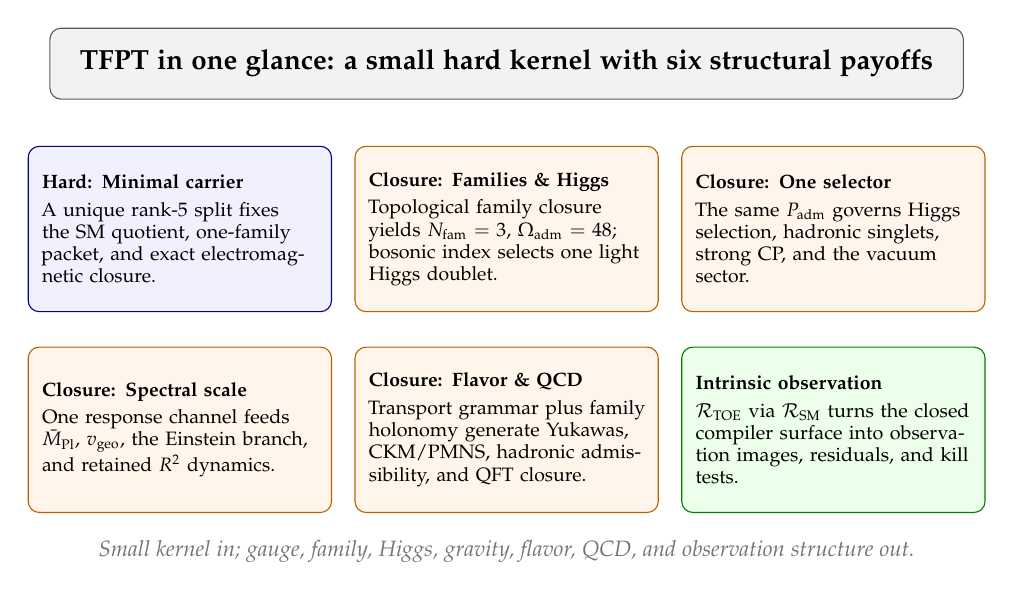
\begin{tikzpicture}[
    headline/.style={draw=black!65, fill=gray!10, rounded corners, minimum width=11.6cm, minimum height=0.9cm, align=center, font=\bfseries},
    hard/.style={draw=blue!60!black, fill=blue!6, rounded corners, text width=3.5cm, minimum height=2.1cm, align=left, inner sep=5pt, font=\scriptsize},
    closure/.style={draw=orange!75!black, fill=orange!8, rounded corners, text width=3.5cm, minimum height=2.1cm, align=left, inner sep=5pt, font=\scriptsize},
    bridge/.style={draw=green!50!black, fill=green!8, rounded corners, text width=3.5cm, minimum height=2.1cm, align=left, inner sep=5pt, font=\scriptsize},
    note/.style={font=\footnotesize\itshape, text=black!55, align=center}
]
\node[headline] (head) at (0,0) {TFPT in one glance: a small hard kernel with six structural payoffs};

\node[hard] (a) at (-4.15,-2.1) {\textbf{Hard: Minimal carrier}\\[2pt]A unique rank-$5$ split fixes the SM quotient, one-family packet, and exact electromagnetic closure.};
\node[closure] (b) at (0,-2.1) {\textbf{Closure: Families \& Higgs}\\[2pt]Topological family closure yields $N_{\mathrm{fam}}\!=\!3$, $\Omega_{\mathrm{adm}}\!=\!48$; bosonic index selects one light Higgs doublet.};
\node[closure] (c) at (4.15,-2.1) {\textbf{Closure: One selector}\\[2pt]The same $\Padm$ governs Higgs selection, hadronic singlets, strong~CP, and the vacuum sector.};

\node[closure] (d) at (-4.15,-4.65) {\textbf{Closure: Spectral scale}\\[2pt]One response channel feeds $\Mpl$, $\vgeo$, the Einstein branch, and retained $R^2$ dynamics.};
\node[closure] (e) at (0,-4.65) {\textbf{Closure: Flavor \& QCD}\\[2pt]Transport grammar plus family holonomy generate Yukawas, CKM/PMNS, hadronic admissibility, and QFT closure.};
\node[bridge] (f) at (4.15,-4.65) {\textbf{Intrinsic observation}\\[2pt]$\mathcal R_{\mathrm{TOE}}$ via $\mathcal R_{\SM}$ turns the closed compiler surface into observation images, residuals, and kill tests.};

\node[note] at (0,-6.2) {Small kernel in; gauge, family, Higgs, gravity, flavor, QCD, and observation structure out.};
\end{tikzpicture}
\caption{Headline claims of the present draft. The figure is intentionally simpler than the
dependency maps that follow: its job is to put the manuscript's core payoff on one page, while
still keeping the hard / closure / intrinsic-observation split visible.}
\label{fig:tfpt-headline-claims}
\end{figure}

\begin{tcolorbox}[colback=tfptblue!3, colframe=tfptblue, breakable,
    title={TFPT master equation and selectors}, colbacktitle=tfptblue]
\begin{equation}
\label{eq:tfpt-master}
\begin{aligned}
S_{\mathrm{TFPT}}
=
\operatorname{Tr}f\!\left(\frac{D_{\mathrm{rel}}+A_{\Sigma}^{\mathrm{seed}}}{\chiseed}\right)
-
\operatorname{Tr}f\!\left(\frac{D_{\mathrm{ref}}}{\chiseed}\right)
+\frac{i\pi}{2}\Delta\eta_\Sigma,
\qquad
A_{\Sigma}^{\mathrm{seed}}:=\mathcal B_{\mathrm{rel}}\oplus\nabla_{\chiseed}.
\end{aligned}
\end{equation}
\begin{equation}
\label{eq:tfpt-selectors}
\begin{aligned}
\operatorname*{Stat}_{\alpha,\chiseed,e,\wspin}S_{\mathrm{TFPT}}=0,
\qquad
\Padm:=P_{\mathrm{str}}P_{\mathrm{gap}},
\qquad
P_{\mathrm{str}}:=P_{\Seam,+}P_{\mathrm{sing}}P_\Theta,
\\
\operatorname{Ind}_{APS}(D^+_{\mathrm{rel}}\otimes L_F)=3,
\qquad
\operatorname{Ind}^{\Padm}_{\mathrm{rel}}(\mathcal B^+_{E_2})=1,
\qquad
\operatorname{Ind}^{\Padm}_{\mathrm{rel}}(\mathcal B^+_{E_3})=0.
\end{aligned}
\end{equation}
\end{tcolorbox}

The hard carrier theorems below do not require the full closure stack behind
\Cref{eq:tfpt-master,eq:tfpt-selectors}. In the present paper the master equation is the
organizing compiler form, the carrier theorems are hard, and the later closure theorems are
internal statements on the admissible reduced datum rather than extra primitive ontology. At this
overview level the seed package is written as $A_{\Sigma}^{\mathrm{seed}}$; on the later
geometric branch it is reorganized as $A_{\Sigma}^{\mathrm{geo}}$ with
$\chiseed\mapsto\chigeo=\Lambda e^\sigma$.

\begin{tcolorbox}[colback=tfptblue!3, colframe=tfptblue, breakable,
    title={Closed TFPT Chain}, colbacktitle=tfptblue]
\begin{equation}
\label{eq:compiler-chain}
\begin{aligned}
\Tmin^{\mathrm{adm}}
&\Rightarrow
( \Tprim^{\mathrm{kin}},\ E_3\oplus E_2,\ G_{\SM}^{\mathrm{glob}},\ S^+)\\
&\Rightarrow
( \Padm,\ F,\ g,\ \sigma,\ \Phi,\ \nabla_F^\star )\\
&\Rightarrow
x_{\mathrm{core}}^\star
\;\Rightarrow\;
\mathcal R_{\mathrm{TOE}}
\;\Rightarrow\;
(O_{\mathrm{th}},\ \Pred).
\end{aligned}
\end{equation}
\end{tcolorbox}

\begin{tcolorbox}[colback=tfptorange!4, colframe=tfptorange!80!black, breakable,
    title={Closed Theorem Stack in the Present Version}, colbacktitle=tfptorange!85!black]
\begin{gather*}
\Tmin^{\mathrm{adm}}
\;\Rightarrow\;
\Tprim
\;\Rightarrow\;
\text{carrier/kernel}
\;\Rightarrow\;
\text{admissibility + geometry + flavor + vacuum}\\[2pt]
\Rightarrow\;
\text{UV + cosmology}
\;\Rightarrow\;
\mathcal R_{\mathrm{TOE}}
\;\Rightarrow\;
O_{\mathrm{th}}.
\end{gather*}
The main text contains no additional primitive ontology beyond the reduced datum.
Several downstream arrows remain explicitly conditional and are marked as such below.
Optional arithmetic continuations, asymptotic expansions, and horizon language are kept only in appendices.
\end{tcolorbox}

\begin{figure}[t]
\centering
\scriptsize
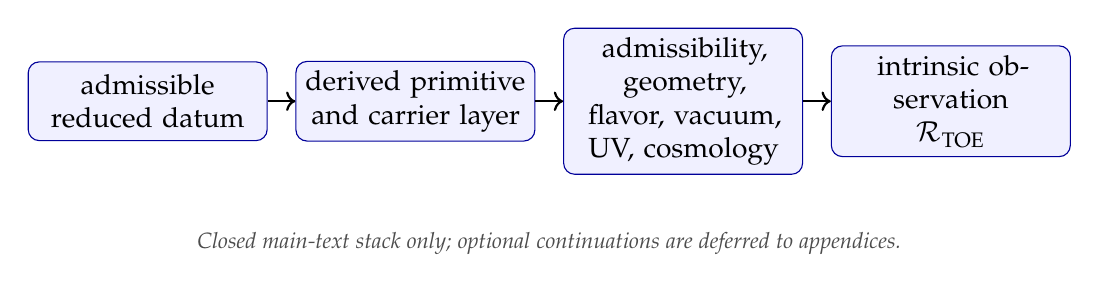
\begin{tikzpicture}[
    closed/.style={draw=blue!60!black, fill=blue!6, rounded corners, text width=2.8cm, minimum height=1.0cm, align=center},
    note/.style={font=\footnotesize\itshape, text=black!70, align=center}
]
\node[closed] (a) at (-5.1,0) {admissible\\reduced datum};
\node[closed] (b) at (-1.7,0) {derived primitive\\and carrier layer};
\node[closed] (c) at (1.7,0) {admissibility, geometry,\\flavor, vacuum, UV, cosmology};
\node[closed] (d) at (5.1,0) {intrinsic observation\\$\mathcal R_{\mathrm{TOE}}$};
\draw[->, thick] (a) -- (b);
\draw[->, thick] (b) -- (c);
\draw[->, thick] (c) -- (d);
\node[note] at (0,-1.8) {Closed main-text stack only; optional continuations are deferred to appendices.};
\end{tikzpicture}
\caption{Closed theorem surface in the present draft. The main text runs from the admissible
reduced datum through the derived closure stack to the intrinsic observation functor, with no
parallel theorem ladder carried in parallel.}
\label{fig:status-ladder}
\end{figure}

The remainder of the main text sharpens each arrow of this chain in turn.

\section{Primitive core and hard carrier kernel}

\subsection{Primitive core and conventions}

We use natural units $c=\hbar=1$. Relative operators are formulated in Euclidean signature and compared through a declared Wick-rotation bridge when Lorentzian language is needed. Higgs fields are denoted by $\Phi$, Hamiltonians by $\mathcal H$, and the cosmological Hubble rate by $\Hhub(t)$; this avoids overloading the letter $H$. Newton's constant is always $G_N$, while $G_{\SM}^{\mathrm{glob}}$ is reserved for the global Standard Model gauge quotient. The seam is denoted by $\Seam$, the involution by $\inv$, and word parity by $\varepsilon(w)$.

Here $S\to \widetilde M$ denotes the spinor bundle on the oriented double cover, and by the same symbol we denote its restriction to
\[
X=\widetilde M\setminus\Seam.
\]

When color-center notation is needed later, we use multiplicative notation
\[
z(w)\in\{1,\omega,\omega^2\},
\qquad
\omega=e^{2\pi i/3}.
\]
Thus center neutrality means $z(w)=1$.

\[
\Tcore^{\mathrm{kin}}
:=
\bigl(
\widetilde M\to M,\ \Seam,\ \inv,\ D_{\mathrm{ref}},\ D_{\mathrm{rel}},\ f,\ \chiseed
\bigr).
\]
When a chosen almost-commutative factorization
$\mathcal H\cong L^2(\widetilde M,S)\otimes\Hint$ is used, $S$ and $\Hint$ refer to that
choice and are not part of the kinematic core datum.
Here \enquote{relative} always means comparison with a declared reference operator or reference-subtracted action. The admissibility predicate $\mathsf{Adm}$ and its operator realization $(\Kadm,\Padm)$ belong to the later closure layer rather than to this primitive bookkeeping package. The technical tables for relative objects, layered closure/benchmark data, and the constants atlas are collected in Appendix~\ref{app:tech} and Appendix~\ref{app:constants}; they are kept out of the early main-text flow so that the carrier kernel appears before the technical bookkeeping apparatus.

\begin{remark}[Reduced datum versus derived structure]
In the present version the oriented double cover, seam, involution, reference/relative
split, and primitive seam response are not additional starting ontology. They are reconstructed
from the admissible reduced datum and then fed into the hard carrier, closure, and intrinsic
observation layers.
\end{remark}

\subsection{Primitive relative spectral dynamics}

The carrier theorem is not intended to float above an unspecified microscopic dynamics.
The starting point is therefore the admissible reduced datum from which the primitive layer is
reconstructed before the later closure theorems are invoked.

\begin{definition}[Admissible reduced theorem datum]
\label{def:reduced-theorem-datum}
The admissible reduced datum is
\[
\Tmin^{\mathrm{adm}}:=(\mathcal A,\mathcal H,D,J,\Gamma,\inv,\nu)
\]
with the following built-in admissibility conditions:
\begin{enumerate}[label=(\roman*), leftmargin=1.5em, topsep=3pt, itemsep=2pt]
    \item $Z(\mathcal A)$ is spectrally regular and its Gelfand spectrum is a smooth compact oriented manifold $\widetilde M$;
    \item $\inv$ acts by a smooth order-two involution on $Z(\mathcal A)$, commutes with $J$ and $\Gamma$, and has smooth fixed locus $\Seam:=\mathrm{Fix}(\inv)$;
    \item in a collar neighborhood of $\Seam$, the Dirac operator has canonical product form
    \[
    D=\gamma_n(\partial_n+B_\Sigma);
    \]
    \item the cutoff profile is generated by a positive complete-Bernstein measure
    \begin{equation}
    \label{eq:bernstein-test-function}
    f(x)=\int_0^\infty e^{-t x^2}\,d\nu(t),
    \qquad
    d\nu(t)\ge 0;
    \end{equation}
    \item the seam collar is reflection-regular so that the doubled operator and admissibility complex defined later are well posed on the same datum.
\end{enumerate}
\end{definition}

\begin{assumption}[Almost commutative factorization of the Hilbert space]
\label{ass:almost-commutative-factorization}
The reduced datum admits an almost commutative factorization
\[
\mathcal H\cong L^2(\widetilde M,S)\otimes \Hint,
\]
with $S\to\widetilde M$ the spinor bundle on the oriented double cover and $\Hint$ a finite
internal Hilbert space.
\end{assumption}

\begin{theorem}[Primitive kinematic scaffold reconstructed from the admissible reduced datum]
\label{thm:primitive-datum-from-reduced-datum}
\label{thm:primitive-scaffold-from-reduced-datum}
Let $\Tmin^{\mathrm{adm}}$ be as above. Then the primitive kinematic scaffold is reconstructed
canonically as
\[
\widetilde M=\mathrm{Spec}\,Z(\mathcal A),\qquad
M=\widetilde M/\inv,\qquad
\Seam=\mathrm{Fix}(\inv),\qquad
X=\widetilde M\setminus \Seam,
\]
\[
D_{\mathrm{ref}}:=\frac12(D+\inv D\inv),\qquad
D_{\mathrm{rel}}:=\frac12(D-\inv D\inv),\qquad
\chiseed:=\lambda_1^+(|B_\Sigma|)^{-1}.
\]
Hence the primitive scaffold
\[
\Tprim^{\mathrm{kin}}
:=
(X,\widetilde M,M,\Seam,\inv,D_{\mathrm{ref}},D_{\mathrm{rel}},f,\chiseed)
\]
is derived, not assumed.
If one further chooses an almost-commutative factorization
\[
\mathcal H_{\mathrm{prim}}\cong L^2(X,S)\otimes \Hint,
\]
then $S$ and $\Hint$ refer to that chosen factorization and are not claimed as
additional reconstruction outputs of the present theorem.
\end{theorem}

\begin{corollary}[No residual primitive topology or comparison-operator ontology]
Within TFPT the oriented double cover, the physical quotient, the seam, the
reference/relative operator pair, and the primitive seam response are theorem-level outputs of
$\Tmin^{\mathrm{adm}}$. Under \Cref{ass:almost-commutative-factorization}, no additional
primitive topology or comparison-operator ontology remains in the main-text scaffold.
\end{corollary}

\begin{definition}[Primitive Euclidean action]
The primitive Euclidean action is the relative spectral seed
\[
S_{\mathrm{prim}}[\chiseed]
:=
\tr f\!\left(\frac{D_{\mathrm{rel}}}{\chiseed}\right)
-
\tr f\!\left(\frac{D_{\mathrm{ref}}}{\chiseed}\right)
+\frac{i\pi}{2}\Delta\eta_\Sigma.
\]
Gauge fixing, ghosts, carrier-compatible bosonic fluctuations, and the admissibly compressed net
\[
\mathfrak A_{\mathrm{adm}}(\mathcal O):=
\Padm\,\mathfrak A(\mathcal O)\,\Padm.
\]
are introduced only after the hard carrier theorem and the later admissibility closure package are in place.
\end{definition}

\begin{theorem}[Bernstein superposition on a positive branch]
\label{ass:bernstein-positivity}
Assume that for every $t>0$ the heat semigroup
\[
e^{-tD_{\mathrm{geo}}^2/\chiseed^2}
\]
is positivity preserving and reflection stable on the seam-even bosonic branch.
If
\[
f(z)=\int_0^\infty e^{-tz^2}\,d\nu(t),\qquad d\nu(t)\ge 0,
\]
then the corresponding Bernstein superposition inherits positivity and reflection stability.
\end{theorem}

\begin{proof}[Proof sketch]
Each heat kernel $e^{-tD_{\mathrm{geo}}^2/\chiseed^2}$ is positivity preserving and reflection
stable on the seam-even bosonic branch by assumption. Positive superposition with
$d\nu(t)\ge 0$ preserves both properties, so the Bernstein profile inherits them immediately.
\end{proof}

\begin{theorem}[Well-posed primitive dynamics]
Assume the geometric anchor admits a self-adjoint Fredholm APS realization on the declared
domain $\APSdom$, and $D_{\mathrm{rel}}$ is relatively bounded with respect to that realization.
Then the finite-cutoff relative spectral seed is well defined before carrier and admissibility
closure are imposed.
\end{theorem}

\begin{proof}[Proof sketch]
Dirac-type operators with APS boundary data admit self-adjoint Fredholm realizations on the
corresponding Sobolev graph domain. Since $D_{\mathrm{rel}}$ is relatively bounded with respect
to the geometric anchor, both operators share the same graph domain and the relative spectral
seed is well defined at every finite cutoff.
\end{proof}

\begin{remark}[APS roles on the admissible branch]
$\APSdom$ is the primitive elliptic boundary choice for the geometric anchor. The family
pairing structure is induced later on the doubled admissible branch and is therefore not a
second primitive input package.
\end{remark}

\begin{figure}[t]
\centering
\scriptsize
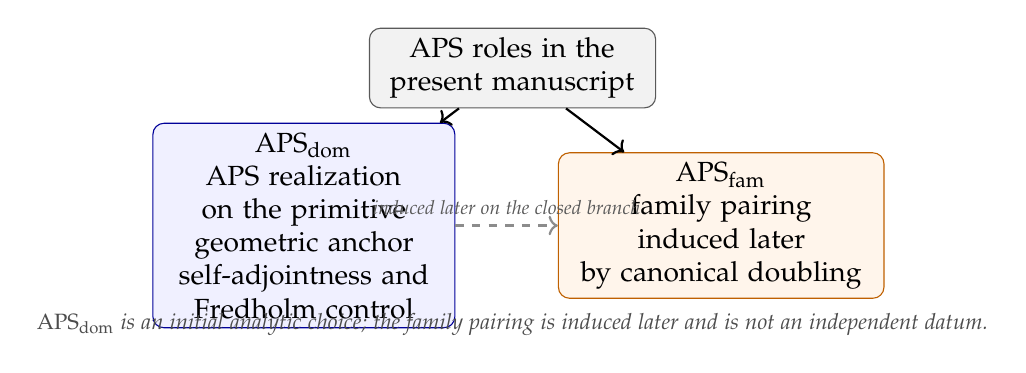
\begin{tikzpicture}[
    root/.style={draw=black!65, fill=gray!10, rounded corners, text width=3.4cm, minimum height=0.9cm, align=center},
    dom/.style={draw=blue!60!black, fill=blue!6, rounded corners, text width=3.6cm, minimum height=1.6cm, align=center},
    fam/.style={draw=orange!75!black, fill=orange!8, rounded corners, text width=3.9cm, minimum height=1.6cm, align=center},
    note/.style={font=\footnotesize\itshape, text=black!70, align=center}
]
\node[root] (aps) at (0,0) {APS roles in the present manuscript};
\node[dom] (dom) at (-2.65,-2.0) {\textbf{$\APSdom$}\\APS realization on the primitive geometric anchor\\self-adjointness and Fredholm control};
\node[fam] (fam) at (2.65,-2.0) {\textbf{$\APSfam$}\\family pairing induced later\\by canonical doubling};
\draw[->, thick] (aps) -- (dom);
\draw[->, thick] (aps) -- (fam);
\draw[->, dashed, black!45, line width=0.8pt] (dom.east) -- node[above, sloped, font=\scriptsize\itshape, text=black!65] {induced later on the closed branch} (fam.west);
\node[note] at (0,-3.25) {$\APSdom$ is an initial analytic choice; the family pairing is induced later and is not an independent datum.};
\end{tikzpicture}
\caption{APS organization in the present draft. $\APSdom$ is the primitive elliptic boundary
choice. The family pairing structure is induced later on the doubled admissible branch and is
therefore not a second primitive input package.}
\label{fig:aps-split}
\end{figure}

\begin{corollary}[Carrier-compatible Lorentzian dynamics after closure]
Once the later carrier-compatible fluctuation package and the admissibility closure hypotheses of \Cref{sec:closure-theorems} are imposed, the resulting admissible Euclidean theory reconstructs a self-adjoint Lorentzian Hamiltonian $H_{\mathrm{adm}}$ and a one-parameter automorphism group
\[
\alpha_t(O)=e^{itH_{\mathrm{adm}}}Oe^{-itH_{\mathrm{adm}}}.
\]
\end{corollary}

\subsection{Minimal carrier theorem}
\label{sec:minimal-carrier-proof}

\begin{theorem}[Minimal carrier theorem]
Let $E=E_b\oplus E_s$ be a split carrier with traceless diagonal generator
\[
Y_{b,s}
=
\mathrm{diag}\!\left(
\underbrace{-\frac1b,\ldots,-\frac1b}_{b\ \text{times}},
\underbrace{\frac1s,\ldots,\frac1s}_{s\ \text{times}}
\right).
\]
If one simultaneously requires
\begin{equation}
\label{eq:minimal-carrier-conditions}
\dim \Lambda^{\mathrm{even}}E=16,
\qquad
\tr_E Y_{b,s}^2=\frac56,
\end{equation}
then necessarily $\{b,s\}=\{3,2\}$.
\end{theorem}

\begin{proof}
Write $g=b+s$. Since
\[
\dim \Lambda^{\mathrm{even}}E=2^{g-1},
\]
the first condition gives $g=5$. For the diagonal generator above one has
\[
\tr_E Y_{b,s}^2
=
b\left(\frac{1}{b^2}\right)+s\left(\frac{1}{s^2}\right)
=
\frac1b+\frac1s
=
\frac{b+s}{bs}
=
\frac{5}{bs}.
\]
Imposing $\tr_E Y_{b,s}^2=5/6$ yields $bs=6$. Together with $b+s=5$ this forces the unordered solution $\{b,s\}=\{3,2\}$.
\end{proof}

Hence from now on
\[
E=E_3\oplus E_2,
\qquad
P_3=\frac{\mathbf 1-\inv}{2},
\qquad
P_2=\frac{\mathbf 1+\inv}{2},
\]
and the hypercharge operator is read concretely as
\begin{equation}
\label{eq:explicit-hypercharge}
Y
=
\mathrm{diag}\!\left(-\frac13,-\frac13,-\frac13,\frac12,\frac12\right)
=
-\frac13 P_3+\frac12 P_2
=
\frac1{12}\mathbf 1+\frac5{12}\inv.
\end{equation}

\begin{lemma}[Hypercharge--seam inversion]
On the minimal carrier, the seam involution is recovered from hypercharge by
\begin{align}
\inv&=\frac{12Y-\mathbf 1}{5},
\label{eq:hypercharge-seam-inversion}\\
(12Y-\mathbf 1)^2&=25\,\mathbf 1,
\nonumber\\
6Y^2-Y-\mathbf 1&=0.
\label{eq:carrier-polynomial}
\end{align}
Consequently the carrier projectors are
\[
P_2=\frac{\mathbf 1+\inv}{2}=\frac{2(3Y+\mathbf 1)}{5},
\qquad
P_3=\frac{\mathbf 1-\inv}{2}=\frac{3(\mathbf 1-2Y)}{5}.
\]
\end{lemma}

\begin{proof}
The affine relation between $Y$ and $\inv$ is inverted algebraically. Squaring the result and using $\inv^2=\mathbf 1$ gives the quadratic carrier polynomial. The projector formulas then follow from $P_2=(\mathbf 1+\inv)/2$ and $P_3=(\mathbf 1-\inv)/2$.
\end{proof}

The hard carrier package is summarized visually in \Cref{fig:minimal-carrier-glance}. The point is that the same minimal data are readable in two equivalent ways: geometrically as an oriented double cover with seam involution, and algebraically as the $3+2$ carrier split with two spectral hypercharges.

\begin{figure}[t]
\centering
\footnotesize
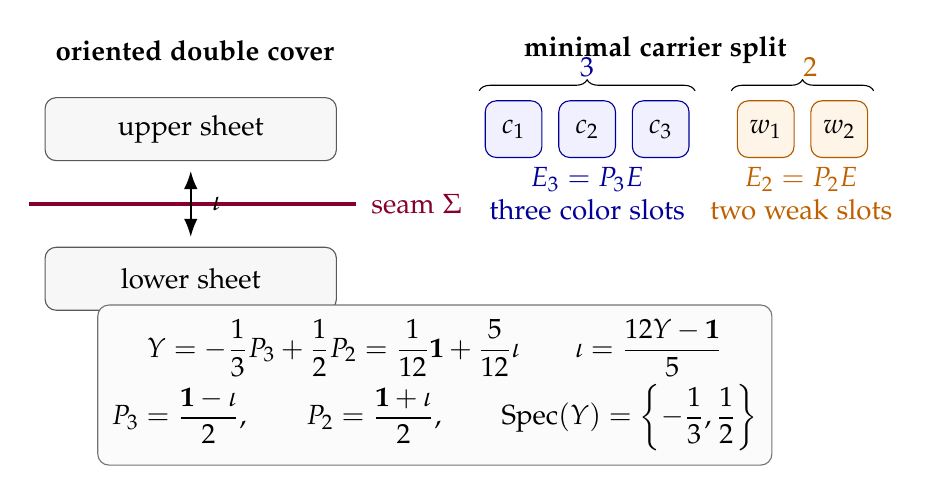
\begin{tikzpicture}[
    >=Latex,
    slot3/.style={draw=blue!60!black, fill=blue!6, rounded corners, minimum width=0.72cm, minimum height=0.72cm, align=center},
    slot2/.style={draw=orange!70!black, fill=orange!9, rounded corners, minimum width=0.72cm, minimum height=0.72cm, align=center},
    info/.style={draw=black!55, rounded corners, fill=gray!3, align=center, inner sep=5pt}
]
\node[font=\bfseries] at (-3.5,1.95) {oriented double cover};
\draw[draw=gray!70!black, fill=gray!6, rounded corners] (-5.4,0.55) rectangle (-1.7,1.35);
\draw[draw=gray!70!black, fill=gray!6, rounded corners] (-5.4,-1.35) rectangle (-1.7,-0.55);
\node at (-3.55,0.95) {upper sheet};
\node at (-3.55,-0.95) {lower sheet};
\draw[very thick, purple!70!black] (-5.6,0) -- (-1.45,0);
\node[anchor=west, purple!70!black] at (-1.38,0) {seam $\Sigma$};
\draw[<->, thick] (-3.55,0.42) -- (-3.55,-0.42);
\node[anchor=west] at (-3.4,0) {$\iota$};

\node[font=\bfseries] at (2.35,1.95) {minimal carrier split};
\node[slot3] (c1) at (0.55,0.95) {$c_1$};
\node[slot3, right=2mm of c1] (c2) {$c_2$};
\node[slot3, right=2mm of c2] (c3) {$c_3$};
\node[slot2, right=6mm of c3] (w1) {$w_1$};
\node[slot2, right=2mm of w1] (w2) {$w_2$};
\node[align=center, blue!60!black] at ($(c2.south)+(0,-0.45)$) {$E_3=P_3E$\\three color slots};
\node[align=center, orange!75!black] at ($(w1.south)+(0.45,-0.45)$) {$E_2=P_2E$\\two weak slots};
\draw[decorate, decoration={brace, amplitude=4pt}] ($(c1.north west)+(-0.07,0.12)$) -- ($(c3.north east)+(0.07,0.12)$);
\node[blue!60!black] at ($(c2.north)+(0,0.42)$) {$3$};
\draw[decorate, decoration={brace, amplitude=4pt}] ($(w1.north west)+(-0.07,0.12)$) -- ($(w2.north east)+(0.07,0.12)$);
\node[orange!75!black] at ($(w1.north east)+(0.2,0.42)$) {$2$};

\node[info] at (-0.45,-2.3) {%
    $\displaystyle
    Y=-\frac13 P_3+\frac12 P_2
    =\frac1{12}\mathbf 1+\frac5{12}\iota
    \qquad
    \iota=\frac{12Y-\mathbf 1}{5}
    $\\[2pt]
    $\displaystyle
    P_3=\frac{\mathbf 1-\iota}{2},
    \qquad
    P_2=\frac{\mathbf 1+\iota}{2},
    \qquad
    \mathrm{Spec}(Y)=\left\{-\frac13,\frac12\right\}
    $};
\end{tikzpicture}
\caption{Minimal carrier at a glance. The seam involution and the hypercharge operator carry the same hard two-point information: geometrically they separate the two sheets, and algebraically they separate the $3+2$ carrier split through the projectors $P_3$ and $P_2$.}
\label{fig:minimal-carrier-glance}
\end{figure}

\begin{remark}[Two-point carrier algebra]
Because the minimal carrier satisfies $6Y^2-Y-\mathbf 1=0$, every analytic function of $Y$ reduces to
\[
f(Y)=A_f\,\mathbf 1+B_f\,Y,
\qquad
A_f=\frac{2f(1/2)+3f(-1/3)}{5},
\qquad
B_f=\frac{6\bigl(f(1/2)-f(-1/3)\bigr)}{5}.
\]
Thus the hard carrier is effectively a two-point algebra supported on the spectral values $-1/3$ and $1/2$, and the projectors $P_3,P_2$ are already polynomial functions of $Y$.
\end{remark}

\begin{remark}[Factorized carrier polynomial and carrier discriminant]\label{rem:carrier-discriminant}
For a general split carrier $E=E_b\oplus E_s$ with total rank $g:=b+s$ and eigenvalues $-1/b$ and $1/s$, the carrier generator satisfies
\[
\left(Y+\frac{1}{b}\right)\left(Y-\frac{1}{s}\right)=0
\quad\Longleftrightarrow\quad
bs\,Y^2+(s-b)Y-\mathbf 1=0.
\]
Its discriminant is
\[
\Delta_Y=(s-b)^2+4bs=(b+s)^2=g^2.
\]
Thus the square root of the carrier discriminant is the carrier rank itself. Moreover,
\[
Y=\frac{b-s}{2bs}\,\mathbf 1+\frac{g}{2bs}\,\inv,
\qquad
\inv=\frac{2bs\,Y-(b-s)\,\mathbf 1}{g}.
\]
On the minimal branch $(b,s)=(3,2)$, this reduces to
\[
6Y^2-Y-\mathbf 1=(2Y-\mathbf 1)(3Y+\mathbf 1),
\qquad
\Delta_Y=25=5^2,
\qquad
\inv=\frac{12Y-\mathbf 1}{5}.
\]
Hence the denominator $5$ in the hypercharge--seam inversion is exactly $\sqrt{\Delta_Y}$, not an additional inserted constant.

This does not replace the stabilizer proof of
\[
G_{\SM}^{\mathrm{glob}}=S(U(3)\times U(2)),
\]
which is the actual source of the global Standard Model quotient in the present manuscript. What the factorization and discriminant do show exactly is that the hard carrier already supports the distinguished spectral values
\[
Y=\frac{1}{2},
\qquad
Y=-\frac{1}{3},
\]
and that the inversion denominator is fixed algebraically by the carrier discriminant.
\end{remark}

The two carrier invariants used repeatedly below are
\[
\gamma=\tr_EY^2=\frac56,
\qquad
B=\frac{\rank E_3}{\rank E_2}=\frac32.
\]
\begin{corollary}[Carrier norm from the carrier polynomial]
The carrier polynomial already fixes
\[
\gamma=\tr_EY^2=\frac16\tr_E(Y+\mathbf 1)=\frac56,
\]
since $\tr_EY=0$ and $\rank E=5$.
\end{corollary}

\begin{corollary}[Minimal carrier compression]
\label{cor:minimal-carrier-compression}
On the minimal carrier branch,
\[
B\gamma=\frac32\cdot\frac56=\frac54.
\]
\end{corollary}

We package the hard kernel as
\[
\Cmin=(E_3\oplus E_2,\ Y,\ S^+,\ \gamma,\ B).
\]

\subsection{Global gauge group and one-family packet}

\begin{theorem}[Global Standard Model theorem]
The determinant-preserving connected stabilizer of the minimal carrier split is
\[
G_{\SM}^{\mathrm{glob}}
=
S(U(3)\times U(2))
\cong
\frac{SU(3)\times SU(2)\times U(1)_Y}{\mathbb Z_6}.
\]
\end{theorem}

\begin{proof}
An automorphism preserving the split $E_3\oplus E_2$ acts by a pair
$(u_3,u_2)\in U(3)\times U(2)$. Requiring determinant preservation on the full
carrier gives
\[
\det(u_3)\det(u_2)=1,
\]
so the connected stabilizer is exactly $S(U(3)\times U(2))$.

Define
\[
\Phi:SU(3)\times SU(2)\times U(1)_Y \longrightarrow S(U(3)\times U(2)),
\qquad
\Phi(g_3,g_2,z)=\bigl(z^2 g_3,\ z^{-3} g_2\bigr).
\]
This is a well-defined group homomorphism because the exponents are integers, and
\[
\det(z^2 g_3)\det(z^{-3} g_2)=z^6 z^{-6}=1.
\]

To prove surjectivity, take $(u_3,u_2)\in S(U(3)\times U(2))$. Choose
$z\in U(1)$ with
\[
z^6=\det(u_3)=\det(u_2)^{-1}.
\]
Then
\[
g_3:=z^{-2}u_3\in SU(3),
\qquad
g_2:=z^{3}u_2\in SU(2),
\]
and therefore
\[
\Phi(g_3,g_2,z)=(u_3,u_2).
\]

If $\Phi(g_3,g_2,z)=(\mathbf 1_3,\mathbf 1_2)$, then
\[
g_3=z^{-2}\mathbf 1_3,
\qquad
g_2=z^{3}\mathbf 1_2.
\]
The conditions $g_3\in SU(3)$ and $g_2\in SU(2)$ imply $z^6=1$. Hence
\[
\ker\Phi
=
\left\{
\bigl(z^{-2}\mathbf 1_3,\ z^{3}\mathbf 1_2,\ z\bigr): z^6=1
\right\}
\cong \mathbb Z_6.
\]
Therefore
\[
S(U(3)\times U(2))
\cong
\frac{SU(3)\times SU(2)\times U(1)_Y}{\mathbb Z_6}.
\]
\end{proof}
This is an internal carrier theorem: it identifies the connected stabilizer of the minimal carrier split. The paper does not claim that the global physical gauge group has already been experimentally fixed at the same level of closure.

Matter is read from the positive half-spinor
\[
S^+=\Lambda^{\mathrm{even}}E,
\qquad
\dim S^+=16.
\]

\begin{theorem}[One carrier family]
The positive half-spinor of the minimal carrier decomposes as
\[
S^+
\cong
(1,1)_0\oplus(3,2)_{1/6}\oplus(\bar 3,1)_{-2/3}\oplus(\bar 3,1)_{1/3}\oplus(1,2)_{-1/2}\oplus(1,1)_1,
\]
that is, exactly one chiral Standard Model family with $\nu^c$. Equivalently, in the familiar unified packaging language,
\[
S^+\cong \mathbf 1\oplus \mathbf{10}\oplus \overline{\mathbf 5}.
\]
\end{theorem}

\begin{proof}
One has
\[
S^+=\Lambda^0E\oplus\Lambda^2E\oplus\Lambda^4E.
\]
The $\Lambda^0E$ sector is immediately
\[
\Lambda^0E\cong (1,1)_0,
\]
which is identified with $\nu^c$ in left-chiral notation. For the minimal carrier,
\[
\Lambda^2E
\cong
\Lambda^2E_3\oplus(E_3\otimes E_2)\oplus\Lambda^2E_2.
\]
Here
\[
\Lambda^2E_3\cong \bar 3,
\qquad
E_3\otimes E_2\cong (3,2),
\qquad
\Lambda^2E_2\cong 1,
\]
and the hypercharges are obtained by adding the carrier charges from
\[
Y=\mathrm{diag}\!\left(-\frac13,-\frac13,-\frac13,\frac12,\frac12\right).
\]
Therefore
\[
\Lambda^2E
\cong
(\bar 3,1)_{-2/3}\oplus(3,2)_{1/6}\oplus(1,1)_1.
\]
Because the full determinant is trivial in $S(U(3)\times U(2))$, one has $\Lambda^5E\cong 1$ and hence
\[
\Lambda^4E\cong E^\ast.
\]
Equivalently,
\[
\Lambda^4E
\cong
(\Lambda^3E_3\otimes E_2)\oplus(\Lambda^2E_3\otimes\Lambda^2E_2).
\]
Using $\Lambda^3E_3\cong 1$, $\Lambda^2E_2\cong 1$, and $\Lambda^2E_3\cong E_3^\ast\cong\bar 3$, one gets
\[
\Lambda^4E\cong (1,2)_{-1/2}\oplus(\bar 3,1)_{1/3}.
\]
Collecting the three even-degree sectors yields
\[
S^+
\cong
(1,1)_0\oplus(\bar 3,1)_{-2/3}\oplus(3,2)_{1/6}\oplus(1,1)_1\oplus(\bar 3,1)_{1/3}\oplus(1,2)_{-1/2},
\]
with total multiplicity $1+3+6+1+3+2=16$. The $\Lambda^2E$ sector is the standard left-chiral $\mathbf{10}$ of $SU(5)$, the $\Lambda^4E$ sector is the standard left-chiral $\overline{\mathbf 5}$, and the $\Lambda^0E$ sector is the singlet $\mathbf 1$.
\end{proof}

In left-chiral notation the one-family decomposition takes the explicit form shown in \Cref{tab:one-family}. This is the place where the manuscript must be explicit: the carrier theorem is meaningful only if the reader can see how the sixteen states are organized.

\begin{table}[t]
\centering
\footnotesize
\begin{tabularx}{\linewidth}{@{}>{\raggedright\arraybackslash}p{0.18\linewidth}>{\raggedright\arraybackslash}p{0.19\linewidth}>{\raggedleft\arraybackslash}p{0.13\linewidth}>{\raggedright\arraybackslash}p{0.20\linewidth}>{\raggedleft\arraybackslash}p{0.08\linewidth}@{}}
\toprule
Exterior component & $\SM$ representation & Hypercharge & Field content & Mult. \\
\midrule
$\Lambda^0E$ & $(1,1)_0$ & $0$ & $\nu^c$ & $1$ \\
$\Lambda^2E_3$ & $(\bar 3,1)_{-2/3}$ & $-2/3$ & $u^c$ & $3$ \\
$E_3\otimes E_2$ & $(3,2)_{1/6}$ & $1/6$ & $Q_L$ & $6$ \\
$\Lambda^2E_2$ & $(1,1)_1$ & $1$ & $e^c$ & $1$ \\
\makecell[l]{$\Lambda^3E_3$\\$\otimes E_2$} & $(1,2)_{-1/2}$ & $-1/2$ & $L_L$ & $2$ \\
\makecell[l]{$\Lambda^2E_3$\\$\otimes\Lambda^2E_2$} & $(\bar 3,1)_{1/3}$ & $1/3$ & $d^c$ & $3$ \\
\midrule
\multicolumn{4}{r}{Total multiplicity} & $16$ \\
\bottomrule
\end{tabularx}
\caption{One chiral family from $S^+=\Lambda^{\mathrm{even}}E$, written in left-chiral notation with charge-conjugate singlets.}
\label{tab:one-family}
\end{table}

\begin{proposition}[Exact parity-code realization of the family packet]
\label{prop:parity-code-family}
Identifying each wedge monomial in $\Lambda E$ with its occupation word
\[
x=(x_1,\dots,x_5)\in\{0,1\}^5,
\]
the positive half-spinor is exactly the even-parity subspace
\[
S^+
\cong
\mathrm{span}\Bigl\{|x\rangle:\sum_{i=1}^5 x_i\equiv 0 \pmod 2\Bigr\}.
\]
Equivalently,
\[
S^+
=
\bigl(\Lambda^{\mathrm{even}}E_3\otimes\Lambda^{\mathrm{even}}E_2\bigr)
\oplus
\bigl(\Lambda^{\mathrm{odd}}E_3\otimes\Lambda^{\mathrm{odd}}E_2\bigr),
\]
and each summand has dimension $8$.
\end{proposition}

\begin{proof}
Choose a basis of $E$ adapted to the split $E_3\oplus E_2$. Exterior monomials are then in bijection with occupation words $x\in\{0,1\}^5$, and the exterior degree is exactly the Hamming weight $\sum_i x_i$. Hence $\Lambda^{\mathrm{even}}E$ is the span of the even-parity words. Splitting the degree into the $E_3$ and $E_2$ contributions gives the direct-sum decomposition above. Since
\[
\dim \Lambda^{\mathrm{even}}E_3=1+\binom32=4,
\qquad
\dim \Lambda^{\mathrm{odd}}E_3=\binom31+\binom33=4,
\]
and
\[
\dim \Lambda^{\mathrm{even}}E_2=1+\binom22=2,
\qquad
\dim \Lambda^{\mathrm{odd}}E_2=\binom21=2,
\]
each tensor-product sector has dimension $8$.
\end{proof}

\begin{remark}[Exact parity lock, not a loose code analogy]
The family packet is therefore not merely code-like: at the level of occupation kinematics it is exactly the classical even-parity $[5,4,2]$ code on five bits. What the present paper still does \emph{not} claim is a dynamical error-correction theorem for realistic noise channels. The exact statement is the parity lock itself. In the maximally mixed state on the $16$ occupation words, eight states lie in the $(\mathrm{even},\mathrm{even})$ sector and eight in $(\mathrm{odd},\mathrm{odd})$, so the coarse parity observables of the $3$-side and $2$-side carry exactly one bit of mutual information.
\end{remark}

The family packet can also be read as a two-dimensional occupancy map, shown in \Cref{fig:family-occupancy-map}. This is where the one-family table, the even-parity code, the split weight enumerator, and the $X=6Y$ arithmetic all meet in one glance.

\begin{figure}[t]
\centering
\footnotesize
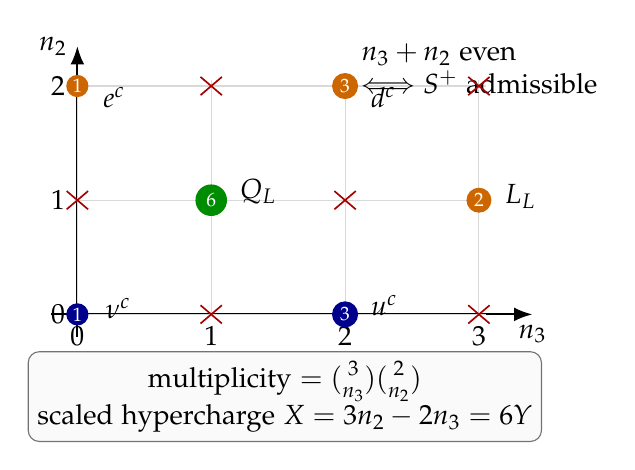
\begin{tikzpicture}[>=Latex, x=1.7cm, y=1.45cm]
\draw[->, thick] (-0.2,0) -- (3.4,0) node[below] {$n_3$};
\draw[->, thick] (0,-0.2) -- (0,2.35) node[left] {$n_2$};
\foreach \x in {0,1,2,3} {
    \draw[gray!30] (\x,0) -- (\x,2.05);
    \node[below] at (\x,-0.02) {\x};
}
\foreach \y in {0,1,2} {
    \draw[gray!30] (0,\y) -- (3.05,\y);
    \node[left] at (-0.02,\y) {\y};
}
\node[align=left, anchor=west] at (2.05,2.15) {$n_3+n_2$ even\\$\Longleftrightarrow S^+$ admissible};

\foreach \x/\y in {1/0,3/0,0/1,2/1,1/2,3/2} {
    \draw[red!65!black, line width=0.6pt] (\x-0.08,\y-0.08) -- (\x+0.08,\y+0.08);
    \draw[red!65!black, line width=0.6pt] (\x-0.08,\y+0.08) -- (\x+0.08,\y-0.08);
}

\filldraw[blue!55!black] (0,0) circle (3.8pt);
\node[text=white, font=\scriptsize] at (0,0) {1};
\node[anchor=west] at (0.14,0.05) {$\nu^c$};

\filldraw[blue!55!black] (2,0) circle (4.5pt);
\node[text=white, font=\scriptsize] at (2,0) {3};
\node[anchor=west] at (2.12,0.08) {$u^c$};

\filldraw[green!55!black] (1,1) circle (5.5pt);
\node[text=white, font=\scriptsize] at (1,1) {6};
\node[anchor=west] at (1.14,1.08) {$Q_L$};

\filldraw[orange!80!black] (0,2) circle (3.8pt);
\node[text=white, font=\scriptsize] at (0,2) {1};
\node[anchor=west] at (0.12,1.9) {$e^c$};

\filldraw[orange!80!black] (3,1) circle (4.3pt);
\node[text=white, font=\scriptsize] at (3,1) {2};
\node[anchor=west] at (3.12,1.03) {$L_L$};

\filldraw[orange!80!black] (2,2) circle (4.5pt);
\node[text=white, font=\scriptsize] at (2,2) {3};
\node[anchor=west] at (2.12,1.9) {$d^c$};

\node[draw=black!55, rounded corners, fill=gray!4, align=center] at (1.55,-0.72) {%
    multiplicity $=\binom{3}{n_3}\binom{2}{n_2}$\\
    scaled hypercharge $X=3n_2-2n_3=6Y$};
\end{tikzpicture}
\caption{Occupancy map of the family packet. The admissible sectors are exactly the even lattice points in $(n_3,n_2)$, with multiplicities $(1,3,6,1,2,3)$ and field labels matching \Cref{tab:one-family}. This is the visual meeting point of parity lock, split weight enumerator, and family hypercharge arithmetic.}
\label{fig:family-occupancy-map}
\end{figure}

\subsection{Character, trace identities, and the abelian index}

\begin{proposition}[Split weight enumerator and one-family character]
\label{prop:split-weight-enumerator}
For the present paragraph let
\[
\chi_{S^+}(t):=\tr_{S^+}(e^{tY}).
\]
Define also the split weight enumerator
\[
W(u,v)
:=
\sum_{\substack{0\le n_3\le 3\\ 0\le n_2\le 2\\ n_3+n_2\ \mathrm{even}}}
\binom{3}{n_3}\binom{2}{n_2}u^{n_3}v^{n_2}.
\]
Then
\begin{equation}
\label{eq:split-weight-enumerator}
W(u,v)
=
1+3u^2+6uv+v^2+2u^3v+3u^2v^2
=
\frac12\Big[(1+u)^3(1+v)^2+(1-u)^3(1-v)^2\Big].
\end{equation}
Moreover,
\begin{equation}
\label{eq:family-character}
\chi_{S^+}(t)
=
\frac12\Big[
\bigl(1+e^{-t/3}\bigr)^3\bigl(1+e^{t/2}\bigr)^2
+
\bigl(1-e^{-t/3}\bigr)^3\bigl(1-e^{t/2}\bigr)^2
\Big]
=
W(e^{-t/3},e^{t/2}).
\end{equation}
Consequently,
\[
\chi_{S^+}(0)=16,
\qquad
\chi_{S^+}'(0)=\tr_{S^+}Y=0,
\qquad
\chi_{S^+}''(0)=\tr_{S^+}Y^2=\frac{10}{3},
\qquad
\chi_{S^+}'''(0)=\tr_{S^+}Y^3=0.
\]
\end{proposition}

\begin{remark}[Master generating function for the one-family packet]
The even-parity split weight enumerator
\[
W(u,v)=\frac12\bigl[(1+u)^3(1+v)^2+(1-u)^3(1-v)^2\bigr]
\]
is the master generator of the family packet. The one-family character is obtained by the
specialization $u=e^{-t/3}$ and $v=e^{t/2}$, while all trace moments of $Y$ are recovered by
differentiating at $t=0$.
\end{remark}

\begin{proof}
The pairs $(n_3,n_2)$ allowed by even total degree are
\[
(0,0),\ (2,0),\ (1,1),\ (0,2),\ (3,1),\ (2,2),
\]
with multiplicities
\[
1,\ 3,\ 6,\ 1,\ 2,\ 3.
\]
This gives the explicit polynomial formula for $W(u,v)$. Equivalently, the parity projector
\[
\frac12\bigl(1+(-1)^{n_3+n_2}\bigr)
\]
acting on $(1+u)^3(1+v)^2$ yields \Cref{eq:split-weight-enumerator}. Substituting
\[
u=e^{-t/3},
\qquad
v=e^{t/2}
\]
gives \Cref{eq:family-character}. For an even exterior algebra one also has
\[
\tr_{\Lambda^{\mathrm{even}}E}(e^{tY})
=
\frac12\Big[\prod_{j=1}^5(1+e^{tq_j})+\prod_{j=1}^5(1-e^{tq_j})\Big],
\]
with carrier charges $q_j\in\{-1/3,-1/3,-1/3,1/2,1/2\}$. Differentiating at $t=0$ yields the stated dimension and trace identities.
\end{proof}

\begin{remark}[Six admissible occupancy sectors]
The six monomials in \Cref{eq:split-weight-enumerator} are exactly the six allowed occupancy pairs $(n_3,n_2)$ of the family packet. This is the shortest combinatorial route from the split carrier to the six Standard Model multiplet sectors listed in \Cref{tab:one-family}.
\end{remark}

The carrier packet therefore reproduces the standard trace cancellations
\[
\tr_{S^+}Y=0,
\qquad
\tr_{S^+}Y^3=0,
\]
and packages them together with the quadratic trace in one formula. Since $\tr_{S^+}Y^2=4\gamma=10/3$ and $\tr_\Phi Y^2=1/2$ for one weak doublet with hypercharge $1/2$, the hypercharge trace coefficient organizes as
\begin{equation}
\label{eq:abelian-index}
\bone(N_{\mathrm{fam}},N_\Phi)
=
\frac25N_{\mathrm{fam}}\tr_{S^+}Y^2+\frac15N_\Phi\tr_\Phi Y^2
=
\frac85N_{\mathrm{fam}}\gamma+\frac1{10}N_\Phi
=
\frac43N_{\mathrm{fam}}+\frac1{10}N_\Phi.
\end{equation}
On the canonical branch $(N_{\mathrm{fam}},N_\Phi)=(3,1)$ this gives
\[
\bone=\frac{41}{10}.
\]
The abelian index is therefore not inserted as an isolated Standard Model datum; it is a carrier-level output once the family and Higgs counts are declared.

\begin{remark}[Canonical-branch Diophantine lock]
If one imposes $\bone=41/10$ on nonnegative integer data, then
\[
40N_{\mathrm{fam}}+3N_\Phi=123.
\]
The physically nontrivial solution is $(N_{\mathrm{fam}},N_\Phi)=(3,1)$, so the canonical branch is already sharply constrained at the level of the trace arithmetic.
\end{remark}

\begin{proposition}[Family hypercharge arithmetic and compression]
\label{prop:family-hypercharge-compression}
Let $N_3$ and $N_2$ be the occupation-number operators on the $E_3$ and $E_2$ slots, restricted to $S^+$, and define the scaled hypercharge operator
\[
X:=6Y=3N_2-2N_3.
\]
Then on $S^+$ one has
\begin{align}
X&\equiv N_2\equiv N_3 \pmod 2,\label{eq:x-mod-2}\\
X&\equiv N_3 \pmod 3,\label{eq:x-mod-3}\\
X&\equiv 3(N_2+N_3) \pmod 5.\label{eq:x-mod-5}
\end{align}
In particular, the even exterior degree $k=N_2+N_3\in\{0,2,4\}$ is read off from the residue class of $X$ modulo $5$: if $X\equiv r\pmod 5$ with $r\in\{0,1,2\}$, then $k=2r$, so
\[
X\bmod 5=0,1,2
\qquad\Longleftrightarrow\qquad
\Lambda^0E,\ \Lambda^2E,\ \Lambda^4E.
\]
Moreover,
\[
\mathrm{Spec}(X|_{S^+})=\{0,-4,1,6,-3,2\},
\]
and therefore
\begin{equation}
\label{eq:family-x-polynomial}
X(X+4)(X-1)(X-6)(X+3)(X-2)=0
\qquad\text{on }S^+.
\end{equation}
\end{proposition}

\begin{proof}
Each occupied $E_3$ mode contributes hypercharge $-1/3$ and each occupied $E_2$ mode contributes $+1/2$, so multiplying by $6$ gives $X=3N_2-2N_3$. Modulo $2$, the term $-2N_3$ vanishes, so $X\equiv N_2$. Because $S^+$ has even total degree, $N_2\equiv N_3\pmod 2$, which proves \Cref{eq:x-mod-2}. Modulo $3$, one has $3N_2\equiv 0$ and $-2\equiv 1$, giving \Cref{eq:x-mod-3}. Modulo $5$, the congruence $-2\equiv 3$ yields \Cref{eq:x-mod-5}. Since on $S^+$ the even degree is $k=N_2+N_3\in\{0,2,4\}$, the possible residues are $3k\equiv 0,1,2\pmod 5$, from which $k=2r$ with $r=X\bmod 5$ follows. Evaluating $X=3n_2-2n_3$ on the six admissible occupancy pairs $(n_3,n_2)$ gives the listed spectrum. The polynomial \Cref{eq:family-x-polynomial} is then the spectral polynomial with these six simple roots.
\end{proof}

\begin{corollary}[Five-fold phase filters for even degree]
\label{cor:family-degree-filters}
Let
\[
\zeta_5=e^{2\pi i/5},
\qquad
U_5:=e^{2\pi iX/5}.
\]
Then the even-degree projectors are the discrete Fourier filters
\[
P_{\Lambda^{2m}E}
=
\frac15\sum_{r=0}^{4}\zeta_5^{-mr}U_5^r,
\qquad
m=0,1,2.
\]
\end{corollary}

\begin{proof}
By \Cref{prop:family-hypercharge-compression}, the eigenspaces $\Lambda^{2m}E$ carry the residue class $X\equiv m\pmod 5$. Hence $U_5$ has eigenvalue $\zeta_5^m$ on $\Lambda^{2m}E$, and the standard Fourier projector formula on the cyclic group $\mathbb Z_5$ gives the claim.
\end{proof}

\begin{remark}[From the two-point carrier to the six-point family algebra]
The minimal carrier itself is a two-point algebra, but the family packet lifts the scaled hypercharge to a six-point algebra. Therefore every analytic function of $X$ on $S^+$ reduces to a polynomial of degree at most five. If
\[
M_n:=\tr_{S^+}(X^n),
\]
then \Cref{eq:family-x-polynomial} implies the finite recursion
\[
M_{n+6}
=
2M_{n+5}+31M_{n+4}-20M_{n+3}-156M_{n+2}+144M_{n+1}.
\]
In this sense the whole hypercharge statistics of one family is finitely compressed into six spectral values.
\end{remark}

\section{Kernel numerics and electromagnetic closure}

The carrier-first presentation should not leave the impression that TFPT is hard only at the level of group theory and representation bookkeeping. The numerical kernel already fixes a nontrivial output layer. Here that layer is pulled forward and read as the first established output package of the carrier/compiler architecture rather than as a later list of disconnected constants.

\begin{proposition}[Seam normalization and base opening]
Let the seam loop carry one unit of relative spectral flow,
\[
SF(U_\Seam)=1,
\qquad
\Delta_\Seam=2\pi.
\]
In the relative Chern normalization, the seam constant is
\[
\cthree:=\frac{\Delta_\Seam}{16\pi^2}=\frac{1}{8\pi}.
\]
Moreover the seam-even base opening is the normalized complement of the carrier quadratic norm,
\[
\phibase
:=
\frac{1-\gamma}{\pi}
=
\frac{1-\tr_EY^2}{\pi}
=
\frac{1}{6\pi}.
\]
\end{proposition}

\begin{proof}[Proof sketch]
One unit of seam spectral flow fixes the topological normalization of the relative one-form coefficient. The carrier theorem gives $\gamma=\tr_EY^2=5/6$. The seam-even opening is therefore the normalized complement of the carrier quadratic norm rather than a new independent numerical input.
\end{proof}

\begin{remark}[Interpretive picture of the primitive start state]
At the level of physical intuition, the primitive spectral seed may be read as a minimal nontrivial relative defect state: two sheets, one seam, one elementary relative winding, and an undecomposed internal rank-$5$ kernel before the carrier split is imposed. This is only an interpretive picture, not a new theorem. Its role is to explain why the earliest hard numbers $(\cthree,\phibase)$ already look like seam-normalized responses of a genuinely relative starting configuration.
\end{remark}

\begin{figure}[t]
\centering
\scriptsize
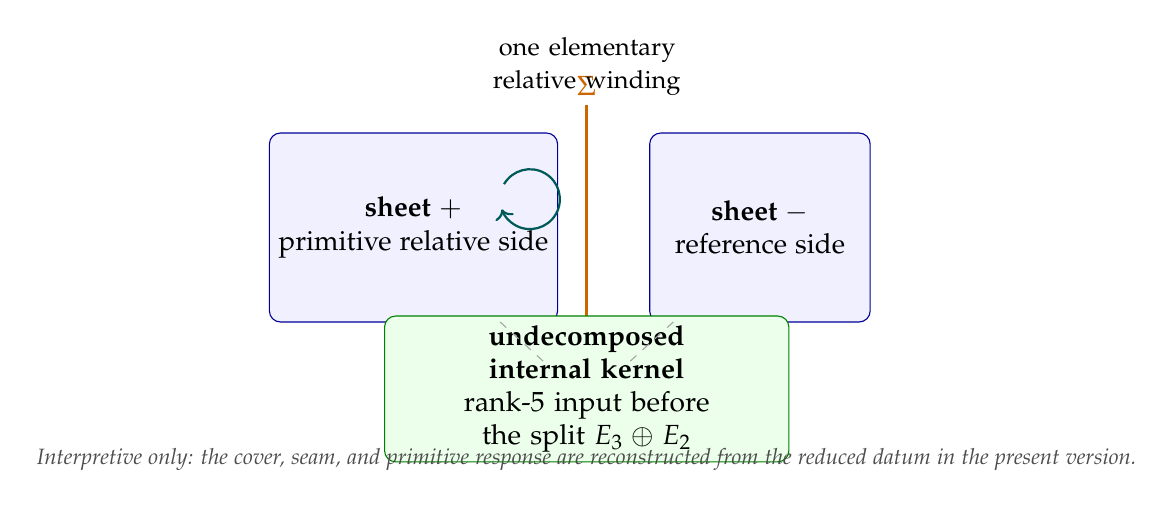
\begin{tikzpicture}[
    sheet/.style={draw=blue!60!black, fill=blue!6, rounded corners, minimum width=2.8cm, minimum height=2.4cm, align=center},
    kernel/.style={draw=green!50!black, fill=green!8, rounded corners, text width=4.9cm, minimum height=0.95cm, align=center},
    note/.style={font=\footnotesize\itshape, text=black!70, align=center}
]
\node[sheet] (up) at (-2.2,0) {\textbf{sheet $+$}\\primitive relative side};
\node[sheet] (down) at (2.2,0) {\textbf{sheet $-$}\\reference side};
\draw[orange!80!black, line width=1.2pt] (0,-1.55) -- (0,1.55);
\node[orange!80!black, above] at (0,1.55) {$\Seam$};
\draw[->, thick, teal!70!black] (-1.05,0.55) arc[start angle=150,end angle=-160,radius=0.38];
\node[align=center, text width=3.4cm] at (0,2.05) {\small one elementary\\relative winding};
\node[kernel] (k) at (0,-2.05) {\textbf{undecomposed internal kernel}\\rank-$5$ input before the split $E_3\oplus E_2$};
\draw[dashed, gray!70] (-1.1,-1.2) -- (-0.55,-1.7);
\draw[dashed, gray!70] (1.1,-1.2) -- (0.55,-1.7);
\node[note] at (0,-2.95) {Interpretive only: the cover, seam, and primitive response are reconstructed from the reduced datum in the present version.};
\end{tikzpicture}
\caption{Interpretive primitive start sketch. The early seam constants are attached to a minimal relative picture with two sheets, one seam, one elementary winding, and an internal rank-$5$ kernel before the split into $E_3\oplus E_2$ is derived.}
\label{fig:primitive-start-sketch}
\end{figure}

\subsection{Carrier form of the electromagnetic closure}

On the canonical admissible branch the inherited topological corrections are
\begin{equation}
\label{eq:hard-topological-kernel}
\deltatop=\frac{3}{256\pi^4},
\qquad
\delta_2=\frac54\,\deltatop^2.
\end{equation}
Numerically,
\[
\cthree=\frac{1}{8\pi}\approx \num{0.03978873577},
\qquad
\deltatop\approx \num{1.2030448e-4},
\qquad
\delta_2\approx \num{1.80914597e-8}.
\]
\begin{definition}[Exact seam generating function]
\label{def:exact-seam-generating-function}
Let
\[
x:=e^{-2\alpha}.
\]
Define the exact seam opening by
\begin{equation}
\label{eq:phi-opening}
\phiseam(\alpha)
:=
\phibase+\deltatop x(1-\deltatop x)^{-5/4}.
\end{equation}
Its Taylor expansion on the admissible branch begins as
\[
\phiseam(\alpha)
=
\phibase
+\deltatop e^{-2\alpha}
+\frac54\deltatop^2e^{-4\alpha}
+O(e^{-6\alpha}),
\]
so the former quadratic opening is retained only as the $n\le 2$ asymptotic truncation of the exact seam generating function.
\end{definition}

\begin{theorem}[Exact electromagnetic closure]
\label{thm:exact-electromagnetic-closure}
The fine-structure constant on the canonical admissible branch is the unique positive solution of
\refstepcounter{equation}\label{eq:carrier-cfe}
\[
\alpha^3
-2\cthree^3\alpha^2
-8\cthree^6\,\bone(N_{\mathrm{fam}},N_\Phi)
\ln\!\bigl((\phiseam(\alpha))^{-1}\bigr)\tag{\theequation}
=0.
\]
\end{theorem}

\begin{corollary}[Second-order asymptotic form]
The former opening
\[
\phibase+\deltatop e^{-2\alpha}+\delta_2e^{-4\alpha}
\]
is the second-order asymptotic expansion of the exact seam generating function
$\phiseam(\alpha)$ and should be used only for asymptotic discussion, not for the benchmark definition.
\end{corollary}

On the canonical family branch these hard coefficients admit the bridge reinterpretations
\[
\Oadm=48,
\qquad
\bone=\frac{41}{10},
\qquad
\deltatop=\Oadm\,\cthree^4,
\qquad
\delta_2=B\gamma\,\Oadm^2\cthree^8=\frac54\,\deltatop^2.
\]

On the canonical branch this is the explicit scalar equation
\[
\alpha^3-\frac{\alpha^2}{256\pi^3}-\frac{41}{327680\pi^6}\ln\!\bigl((\phiseam(\alpha))^{-1}\bigr)=0.
\]

The dependency structure of the electromagnetic closure is displayed in \Cref{fig:alpha-closure-flow}. What matters is not one formula in isolation, but the fact that the same carrier-side inputs fix both the exact seam opening and the self-consistent root.
\begin{remark}[Logarithmic scale closure of the electromagnetic equation]
Define the internally generated logarithmic scale
\[
\mu_\Sigma(\alpha):=(\phiseam(\alpha))^{-1}.
\]
Then \Cref{eq:carrier-cfe} is equivalent to
\[
\ln \mu_\Sigma(\alpha)
=
\frac{\alpha^2\bigl(\alpha-2\cthree^3\bigr)}
{8\cthree^6\,\bone(N_{\mathrm{fam}},N_\Phi)}.
\]
Thus the observed fine-structure constant is selected by a balance between a geometric cubic term
and a self-generated logarithmic scale parameter. This is RG-like and transmutation-like,
because $\bone$ is the abelian trace coefficient and the logarithm is attached to an internally
produced scale. In the present paper it should be read as \emph{logarithmic scale closure} or a
geometric fixed-point equation rather than as an externally prescribed one-loop running law. The
symbol $\mu_\Sigma(\alpha)$ here is local to the electromagnetic closure discussion and should
not be confused with the later matching scale $M_\Sigma$.
\end{remark}
A related appendix continuation records that
\[
\gcd(\Oadm,\Dstart)=\dim \mathfrak g_{\SM},
\qquad
\operatorname{lcm}(\Oadm,\Dstart)=|R(E_8)|.
\]

\begin{figure}[t]
\centering
\scriptsize
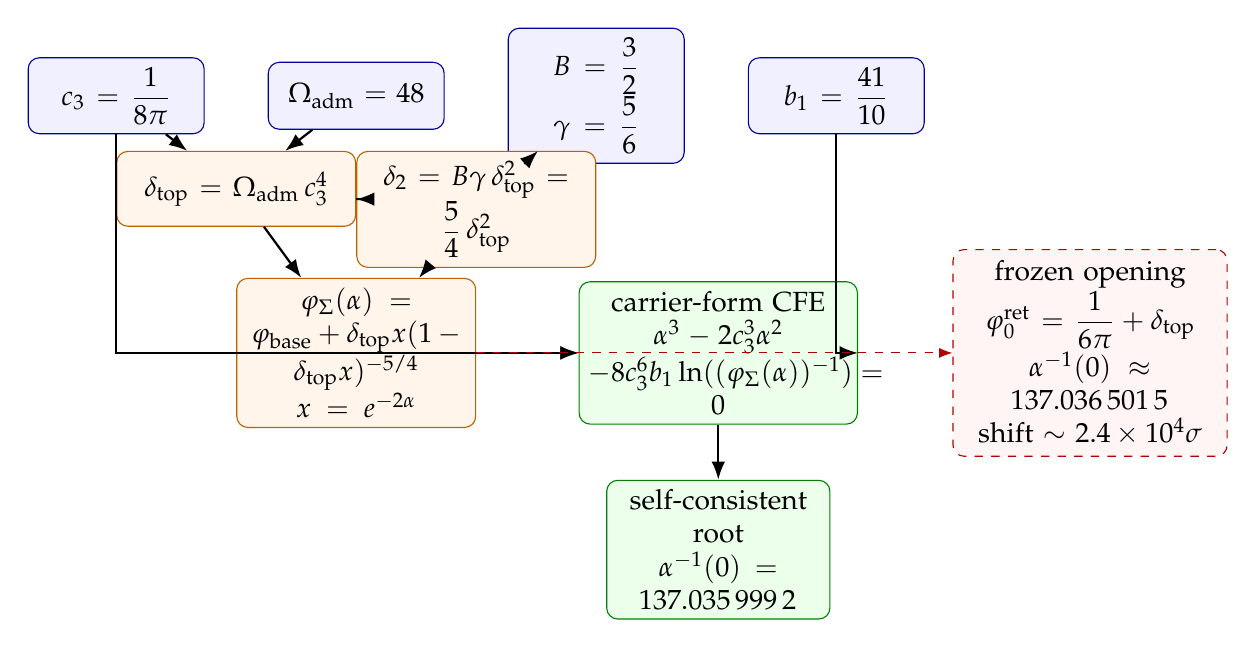
\begin{tikzpicture}[
    >=Latex,
    node distance=7mm and 8mm,
    hard/.style={draw=blue!60!black, fill=blue!6, rounded corners, align=center, text width=2.0cm, minimum height=0.85cm},
    closure/.style={draw=orange!75!black, fill=orange!8, rounded corners, align=center, text width=2.8cm, minimum height=0.95cm},
    outbox/.style={draw=green!50!black, fill=green!8, rounded corners, align=center, text width=2.6cm, minimum height=0.95cm},
    note/.style={draw=red!70!black, dashed, rounded corners, fill=red!4, align=center, text width=3.2cm, inner sep=4pt}
]
\node[hard] (c3) {$\cthree=\dfrac{1}{8\pi}$};
\node[hard, right=of c3] (omega) {$\Oadm=48$};
\node[hard, right=of omega] (bg) {$B=\dfrac32$\\$\gamma=\dfrac56$};
\node[hard, right=of bg] (b1) {$\bone=\dfrac{41}{10}$};

\node[closure, below=of $(c3)!0.5!(omega)$] (dtop) {$\deltatop=\Oadm\,\cthree^4$};
\node[closure, below=of $(omega)!0.5!(bg)$] (dtwo) {$\delta_2=B\gamma\,\deltatop^2=\dfrac54\,\deltatop^2$};
\node[closure, below=of $(dtop)!0.5!(dtwo)$, yshift=-3mm] (phi) {$\phiseam(\alpha)=\phibase+\deltatop x(1-\deltatop x)^{-5/4}$\\$x=e^{-2\alpha}$};
\node[outbox, text width=3.3cm, right=13mm of phi] (cfe) {carrier-form CFE\\$\alpha^3-2\cthree^3\alpha^2$\\$-8\cthree^6\bone\ln((\phiseam(\alpha))^{-1})=0$};
\node[outbox, below=of cfe] (root) {self-consistent root\\$\alpha^{-1}(0)=\num{137.0359992}$};
\node[note, right=12mm of cfe] (frozen) {frozen opening\\$\phiz=\dfrac{1}{6\pi}+\deltatop$\\$\alpha^{-1}(0)\approx\num{137.0365015}$\\shift $\sim \num{2.4e4}\sigma$};

\draw[->, thick] (c3) -- (dtop);
\draw[->, thick] (omega) -- (dtop);
\draw[->, thick] (dtop) -- (dtwo);
\draw[->, thick] (bg) -- (dtwo);
\draw[->, thick] (dtop) -- (phi);
\draw[->, thick] (dtwo) -- (phi);
\draw[->, thick] (c3) |- (cfe);
\draw[->, thick] (b1) |- (cfe);
\draw[->, thick] (phi) -- (cfe);
\draw[->, thick] (cfe) -- (root);
\draw[->, dashed, red!70!black] (phi.east) -- (frozen.west);
\end{tikzpicture}
\caption{$\alpha$ closure flow. Carrier-side integers and minimal-carrier invariants feed the defect terms, those defect terms feed the exact seam generating function $\phiseam(\alpha)$, and only the self-consistent loop gives the benchmark root. The dashed inset shows why a frozen opening is not a harmless simplification.}
\label{fig:alpha-closure-flow}
\end{figure}

\subsection{Kernel output package}

The benchmark row for $\alpha^{-1}(0)$ is defined by the positive self-consistent root of \Cref{eq:carrier-cfe}, not by freezing the opening at its retained seed value. On the canonical branch that positive root remains
\[
\alpha^{-1}(0)=\num{137.03599921615843}.
\]
For the remaining one-seed relations we keep the retained branch opening
\begin{equation}
\label{eq:hard-kernel-values}
\cthree=\frac{1}{8\pi},
\qquad
\phiz=\frac{1}{6\pi}+\frac{3}{256\pi^4},
\end{equation}
\begin{remark}[Exact opening versus retained seed]
The two symbols belong to the same admissible branch but play different jobs. The electromagnetic $\alpha$ row uses the exact seam generating function $\phiseam(\alpha)$ inside the carrier-form closure equation, whereas the one-seed bridge relations freeze that branch to the retained canonical seed $\phiz$. Thus $\phiseam(\alpha)$ belongs only to the exact $\alpha$ benchmark line, while $\phiz$ is the seed used for $(\beta_{\mathrm{rad}},\Omega_b,\lambda_C,\sin^2\theta_{13})$.
\end{remark}
and the same retained kernel package emits the compact seed chain
\begin{equation}
\label{eq:kernel-benchmark-formulas}
C_{a\gamma\gamma}=-4\cthree=-\frac{1}{2\pi},
\qquad
\beta_{\mathrm{rad}}=\frac{\phiz}{4\pi},
\qquad
\Omega_b=(4\pi-1)\beta_{\mathrm{rad}},
\qquad
\lambda_C=\sqrt{\phiz(1-\phiz)},
\qquad
\sin^2\theta_{13}=\phiz e^{-\gamma}.
\end{equation}
\begin{remark}[Why the $\alpha$ row must stay self-consistent]
The benchmark number $\alpha^{-1}(0)=\num{137.03599921615843}$ comes from the exact self-consistent equation with $\phiseam(\alpha)$. Its second-order truncation reproduces the first two correction coefficients, but it is not itself the benchmark definition. If one instead freezes the opening at
\[
\phiz=\frac{1}{6\pi}+\frac{3}{256\pi^4},
\]
the root shifts to $\alpha^{-1}(0)\approx \num{137.036501465}$, i.e. by about $\num{5.02e-4}$, which is roughly $\num{2.4e4}\sigma$ on the CODATA/NIST uncertainty. The wording of the $\alpha$ benchmark must therefore remain explicit: the benchmark uses the exact seam generating function, while the quadratic formula is only its controlled asymptotic shadow.
\end{remark}
\begin{tcolorbox}[colback=tfptblue!3, colframe=tfptblue, breakable,
    title={Kernel-output package}, colbacktitle=tfptblue]
The point of this section is not to claim more numerics than TFPT currently owns. It is to show that the established kernel already fixes a coherent electromagnetic package before the later completion theorems begin: the seam constant $\cthree$, the retained canonical seed $\phiz$, the self-consistent carrier-form CFE for $\alpha$, the dimensionless axion--photon anomaly coefficient, the birefringence seed, and the Cabibbo anchor.
\end{tcolorbox}

\section{Compression identities and carrier exclusion}

This section collects the algebraic compressions that turn the carrier packet and kernel numerics from a list of internally consistent outputs into an overdetermined structure with genuine exclusion power. The compression identities are not new theorems; they are exact algebraic consequences of the already established carrier data. The exclusion theorems are the sharpest available evidence that the carrier packet actively selects the physical world.

\subsection{Rank lock and the \texorpdfstring{$2$-$3$-$5$}{2-3-5} arithmetic}

\begin{proposition}[Carrier rank lock]
\label{prop:rank-lock}
If the carrier identity $\dim S^+=2^{g-1}$, the canonical family data $N_{\mathrm{fam}}=3$, and the optional occupancy compression $\Oadm=(g-1)\dim\mathfrak g_{\SM}=12(g-1)$ are combined, then
\begin{equation}
\label{eq:rank-lock}
3\cdot 2^{g-1}=12(g-1)
\qquad\Longleftrightarrow\qquad
2^{g-3}=g-1.
\end{equation}
The unique integral solution is $g=5$.
\end{proposition}

\begin{proof}
Set $f(g):=2^{g-3}-(g-1)$. Then
\[
f(1)=\frac14,\qquad
f(2)=-\frac12,\qquad
f(3)=-1,\qquad
f(4)=-1,\qquad
f(5)=0.
\]
For $g\ge 4$,
\[
f(g+1)-f(g)=2^{g-3}-1>0,
\]
so $f$ is strictly increasing on $g\ge 4$. Since $f(4)<0$ and $f(5)=0$, there is no solution with $g\ge 6$. A direct check for $g\le 4$ shows no other solution. Hence the unique integral solution is $g=5$.
\end{proof}

\begin{remark}[The $2$-$3$-$5$ arithmetic]
The hard carrier packet rests on exactly three discrete numbers: $2$ (the double cover), $3$ (the color rank and family count), and $5$ (the carrier rank). From these three atoms one recovers
\[
\gamma=\frac{5}{6}=\frac{5}{2\cdot 3},
\qquad
B=\frac{3}{2},
\qquad
B\gamma=\frac{5}{4}=\frac{5}{2^2},
\]
\[
\Oadm=3\cdot 2^4=48,
\qquad
\Dstart=5\cdot 12=60,
\qquad
\frac{\Dstart}{\Oadm}=\frac{5}{4}=B\gamma,
\]
and the defect coefficients $\deltatop=48\,\cthree^4$ and $\delta_2=\frac54\,\deltatop^2=2880\,\cthree^8$ with $2880=60\cdot 48$.
The persistent appearance of $5/4$ as carrier asymmetry $\times$ norm, second defect stage, and ladder-to-occupancy ratio is therefore not three coincidences but one rational shadow of the $2$-$3$-$5$ triad.
\end{remark}

\begin{lemma}[Universal \texorpdfstring{$5/4$}{5/4} compression quotient on the minimal branch]
\label{lem:universal-5-4-compression}
Define
\[
\rho_{5/4}:=B\gamma.
\]
On the canonical minimal branch,
\[
\rho_{5/4}
=
B\gamma
=
\frac{\delta_2}{\deltatop^2}
=
\frac{\Dstart}{\Oadm}
=
\frac{\gcar}{\gcar-1}
=
\frac54.
\]
Thus $5/4$ is the universal compression quotient of the minimal branch rather than a recurring numerical motif.
\end{lemma}

\begin{proof}
The identity $B\gamma=\frac54$ is \Cref{cor:minimal-carrier-compression}. The defect relation gives
\[
\frac{\delta_2}{\deltatop^2}=\frac54.
\]
On the canonical branch,
\[
\frac{\Dstart}{\Oadm}=\frac{60}{48}=\frac54,
\]
and with $\gcar=5$ one also has
\[
\frac{\gcar}{\gcar-1}=\frac{5}{4}.
\]
Hence all displayed ratios agree on the same exact value.
\end{proof}

\begin{remark}[Interpretive status of the quotient]
The quotient itself is exact. Any holographic or spacetime-dimensional reading of the denominator $\gcar-1=4$ remains interpretive in the present manuscript rather than theorem-level.
\end{remark}

\begin{remark}[Rank-5 master compression]
If one accepts the carrier rank as the master parameter, then on the canonical branch
\[
N_{\mathrm{fam}}=\frac{\gcar+1}{2}=3,
\qquad
\Oadm=N_{\mathrm{fam}}\,2^{\gcar-1}=\frac{(\gcar+1)}{2}\,2^{\gcar-1}=(\gcar+1)\,2^{\gcar-2}=48,
\]
\[
\Oadm\gamma=\gcar\,2^{\gcar-2}=40,
\qquad
\bone=\frac{\gcar\,2^{\gcar-2}+1}{10}=\frac{41}{10}.
\]
This is an algebraic compression of the closed family count, occupancy, abelian index, and the
$41$-chain onto the single integer $\gcar=5$.
\end{remark}

\begin{corollary}[Pythagorean compression of the integrity index on the rank-locked branch]
\label{cor:pythagorean-integrity-index}
Assume the rank-locked compression branch
\[
10\,\bone=\gcar\,2^{\gcar-2}+1
\]
and the rank lock
\[
2^{\gcar-3}=\gcar-1.
\]
Then
\[
\mathcal I_{41}
=
10\,\bone
=
2\gcar(\gcar-1)+1
=
\gcar^2+(\gcar-1)^2.
\]
In particular, on the minimal rank-locked branch $\gcar=5$ one gets
\[
\mathcal I_{41}=5^2+4^2=41.
\]
\end{corollary}

\begin{proof}
Multiplying the rank lock by $2\gcar$ gives
\[
\gcar\,2^{\gcar-2}=2\gcar(\gcar-1).
\]
Inserting this into the compression formula yields
\[
10\,\bone=2\gcar(\gcar-1)+1.
\]
Since
\[
2\gcar(\gcar-1)+1=\gcar^2+(\gcar-1)^2,
\]
the claim follows.
\end{proof}

\begin{remark}[The number $4$ as a cross-cutting echo]
In addition to the $2$-$3$-$5$ triad, the integer $4$ appears at four structurally distinct levels:
\[
F_{\mathrm{patch}}=4,
\qquad
\gcar-1=4,
\qquad
\frac{\Oadm}{\dim\mathfrak g_{\SM}}=\frac{48}{12}=4,
\qquad
\frac{|R(E_8)|}{\Dstart}=\frac{240}{60}=4.
\]
That is, four corner patches, carrier rank minus one, matter-to-gauge compression factor, and root-to-start quotient all evaluate to the same integer.
\end{remark}

\subsection{Exact algebraic compressions on the minimal branch}

\begin{corollary}[Two-point spectral compression of $\gamma$ and $\phibase$]
Let
\[
y_+:=\frac12,
\qquad
y_-:=-\frac13
\]
be the two distinct carrier eigenvalues singled out by the factorized carrier polynomial. Then
\[
\gamma=y_+-y_-,
\qquad
\phibase=\frac{y_++y_-}{\pi}.
\]
Here $y_++y_-$ is the unweighted Vieta sum of the two distinct carrier eigenvalues, not the trace on $E$.
\end{corollary}

\begin{proof}
By \Cref{eq:carrier-polynomial}, equivalently by the factorization
\[
6Y^2-Y-\mathbf 1=(2Y-\mathbf 1)(3Y+\mathbf 1),
\]
the two distinct carrier eigenvalues are exactly $y_+=1/2$ and $y_-=-1/3$. Their difference is
\[
y_+-y_-=\frac12+\frac13=\frac56=\gamma,
\]
while their sum is
\[
y_++y_-=\frac12-\frac13=\frac16.
\]
Since $\phibase=(1-\gamma)/\pi=1/(6\pi)$, the claim follows.
\end{proof}

\begin{remark}[Carrier root pair formalism]
Let
\[
y_+=\frac12,
\qquad
y_-=-\frac13.
\]
Then all one-family hypercharges are generated by the same two carrier roots:
\[
Y(Q_L)=y_++y_-,
\quad
Y(u^c)=2y_-,
\quad
Y(d^c)=-y_-,
\quad
Y(L_L)=-y_+,
\quad
Y(e^c)=2y_+,
\quad
Y(\nu^c)=0.
\]
Moreover the positive transport cusps satisfy
\[
\left\{1,\frac23,\frac13\right\}=\{2y_+,-2y_-,2(y_++y_-)\}.
\]
Thus the carrier packet and the transport grammar are generated by the same two-point root data.
\end{remark}

\begin{corollary}[Family hypercharge variance and electroweak block trace]
Equip one carrier family with the uniform average
\[
\mathbb E_{S^+}(A):=\frac{1}{16}\tr_{S^+}A.
\]
Then
\[
\operatorname{Var}_{S^+}(Y)
:=
\mathbb E_{S^+}(Y^2)-\mathbb E_{S^+}(Y)^2
=
\frac{1}{16}\tr_{S^+}Y^2
=
\frac{5}{24}.
\]
Consequently,
\[
I_1^{\mathrm{EW}}=\operatorname{Var}_{S^+}(Y)\,\bone.
\]
\end{corollary}

\begin{proof}
The one-family trace identities give $\tr_{S^+}Y=0$ and $\tr_{S^+}Y^2=10/3$. Hence the centered second moment is
\[
\frac{1}{16}\tr_{S^+}Y^2=\frac{10/3}{16}=\frac{5}{24}.
\]
Using $I_1^{\mathrm{EW}}=\frac{5}{24}\,\bone$ from the electroweak block relation yields the second identity.
\end{proof}

\begin{corollary}[Factorial quadratic trace and two-defect factorization]
\label{cor:factorial-trace-delta2}
Let
\[
X:=6Y.
\]
Then the one-family quadratic trace is
\[
\tr_{S^+}(X^2)
=
36\,\tr_{S^+}(Y^2)
=
36\cdot\frac{10}{3}
=
120
=
5!.
\]
Equivalently, using the six hypercharge sectors with multiplicities
\[
(1,3,6,1,2,3)
\]
at
\[
X\in\{0,-4,1,6,-3,2\},
\]
the same trace is
\[
0^2+3\cdot 4^2+6\cdot 1^2+1\cdot 6^2+2\cdot 3^2+3\cdot 2^2=120.
\]
On the retained branch this gives the exact factorization
\[
\delta_2
=
2880\,\cthree^8
=
4!\,\tr_{S^+}(X^2)\,\cthree^8.
\]
\end{corollary}

\begin{proof}
By \Cref{prop:split-weight-enumerator}, one has
\[
\tr_{S^+}(Y^2)=\frac{10}{3}.
\]
Since $X=6Y$, the first identity follows immediately. The sector-by-sector sum is the same quadratic trace written in the basis of admissible occupancy sectors from \Cref{prop:family-hypercharge-compression}. Finally, \Cref{eq:hard-topological-kernel} gives
\[
\delta_2=2880\,\cthree^8=24\cdot 120\,\cthree^8
=
4!\,\tr_{S^+}(X^2)\,\cthree^8.
\]
\end{proof}

\begin{remark}[Quadratic trace versus variance]
The value $120=5!$ is the unnormalized quadratic trace $\tr_{S^+}(X^2)$, not the normalized variance. The corresponding uniform variance is
\[
\operatorname{Var}_{S^+}(X)=36\,\operatorname{Var}_{S^+}(Y)=36\cdot\frac{5}{24}=\frac{15}{2}.
\]
\end{remark}

\begin{remark}[Arithmetic Higgs lock on the canonical family branch]
Define the generic occupancy
\[
\Omega_{\mathrm{occ}}:=16\,N_{\mathrm{fam}}.
\]
Then the abelian-index formula gives
\[
10\,\bone
=
\frac{40}{3}N_{\mathrm{fam}}+N_\Phi
=
\Omega_{\mathrm{occ}}\,\gamma+N_\Phi.
\]
On the canonical family branch $N_{\mathrm{fam}}=3$, hence $\Omega_{\mathrm{occ}}=48$ and therefore
\[
10\,\bone=40+N_\Phi.
\]
Thus the $41$-chain arithmetically selects $N_\Phi=1$. This is an arithmetic lock on the canonical branch, not the dynamical Higgs-selection theorem, which in the present manuscript still comes from the bosonic relative-index / Callias route.
\end{remark}

\subsection{The \texorpdfstring{$41$}{41} integrity index}

The integer $41$ is not an isolated numerical curiosity. On the retained branch it is best read as a weighted integrity index rather than as a topological Euler-type object.
\begin{definition}[The \texorpdfstring{$41$}{41} integrity index]
\label{def:integrity-index-41}
Let
\[
\mathcal I_{41}:=10\,\bone=\Omega_{\mathrm{occ}}\gamma+N_\Phi.
\]
On the canonical branch, $\Omega_{\mathrm{occ}}=\Oadm=48$ and $N_\Phi=1$, so
\[
\mathcal I_{41}=40+1=41.
\]
\end{definition}

Then the hard arithmetic chain reads
\begin{equation}
\label{eq:41-chain-main}
10\,\bone
=
\Oadm\gamma+1
=
41.
\end{equation}
\begin{figure}[t]
\centering
\footnotesize
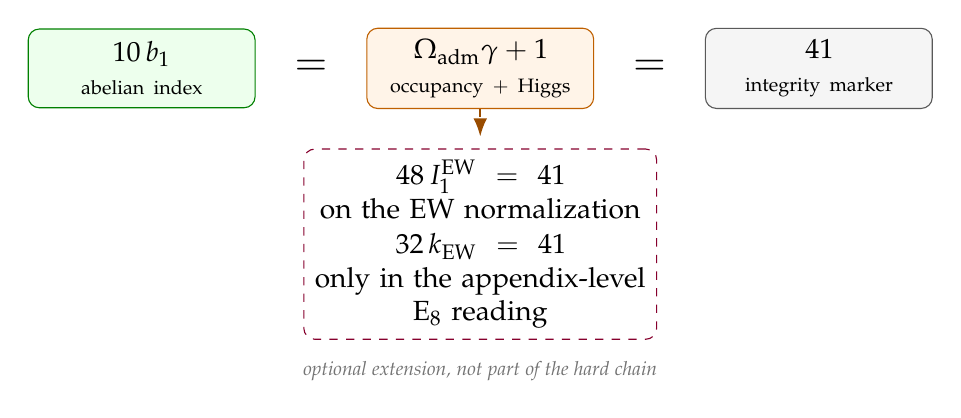
\begin{tikzpicture}[
    >=Latex,
    chain/.style={draw=black!55, rounded corners, align=center, text width=2.6cm, minimum height=1.0cm, inner sep=4pt},
    optchain/.style={draw=purple!70!black, dashed, rounded corners, align=center, text width=4.2cm, minimum height=0.95cm, inner sep=4pt},
    eq/.style={font=\Large},
    note/.style={font=\scriptsize\itshape, text=black!55, align=center}
]
\node[chain, fill=green!7, draw=green!50!black] (a) at (0,0) {$10\,\bone$\\\scriptsize abelian index};
\node[eq] at (2.15,0) {$=$};
\node[chain, fill=orange!9, draw=orange!75!black] (b) at (4.3,0) {$\Oadm\gamma+1$\\\scriptsize occupancy $+$ Higgs};
\node[eq] at (6.45,0) {$=$};
\node[chain, fill=gray!8, draw=black!65] (c) at (8.6,0) {$41$\\\scriptsize integrity marker};
\draw[dashed, orange!60!black, ->, thick] (b.south) -- ++(0,-0.35);
\node[optchain, below=0.5cm of b] (d) {$48\,I_1^{\mathrm{EW}}=41$\\ on the EW normalization\\[1pt]$32\,k_{\mathrm{EW}}=41$\\ only in the appendix-level\\E$_8$ reading};
\node[note, below=0.15cm of d] {optional extension, not part of the hard chain};
\end{tikzpicture}
\caption{The $41$-chain strip. The hard arithmetic chain is $10\,\bone=\Oadm\gamma+1=41$. Electroweak normalization and E$_8$ block-language extensions are shown only as optional downstream readings.}
\label{fig:41-chain-strip}
\end{figure}
The extra $+1$ is precisely the arithmetic contribution of one light seam-even Higgs doublet. This makes $\mathcal I_{41}$ a hypercharge-driven occupancy integrity index:
\[
\mathcal I_{41}=40+1,
\]
with $40=\Oadm\gamma$ the fermionic weighted occupancy and $1=N_\Phi$ the light Higgs contribution. The canonical branch is therefore locked arithmetically at $40\mapsto 41$, while the actual dynamical Higgs-selection theorem still comes from the bosonic / Callias closure route.

\begin{remark}[Optional block-trace extension]
If one introduces the electroweak block normalization
\[
I_1^{\mathrm{EW}}:=\frac{5}{24}\,\bone,
\]
then
\[
48\,I_1^{\mathrm{EW}}=41.
\]
The further identity
\[
32\,k_{\mathrm{EW}}=41
\]
belongs only to the appendix-level E$_8$ reading and requires the block-index extrapolation.
\end{remark}

\begin{remark}[Integrity-index reading]
The canonical branch may be read as carrying an integrity marker: the hypercharge trace coefficient and the occupancy-weighted carrier norm plus one light Higgs doublet collapse onto the same integer $41$. This is not a cryptographic claim. It is an algebraic consistency signature showing that several independently defined carrier-side layers agree on one integer.
\end{remark}

\subsection{Single-seed compression and the Cabibbo inversion}

The seed-driven observation rows $(\beta_{\mathrm{rad}},\Omega_b,\lambda_C,\sin^2\theta_{13})$
are not four independent hits but four projections of $\phiz$. The Cabibbo angle admits an
explicit inversion back to the seed:
\begin{equation}
\label{eq:cabibbo-inversion}
\phiz=\frac{1-\sqrt{1-4\lambda_C^2}}{2}.
\end{equation}
\begin{remark}[Catalan expansion of the Cabibbo inversion]
Setting
\[
x:=\lambda_C^2,
\]
the inversion formula becomes
\[
\phiz=x\,C(x),
\qquad
C(x):=\frac{1-\sqrt{1-4x}}{2x}.
\]
Hence
\begin{equation}
\label{eq:catalan-cabibbo}
\phiz
=
\sum_{n\ge 0} C_n\,\lambda_C^{2n+2}
=
\lambda_C^2+\lambda_C^4+2\lambda_C^6+5\lambda_C^8+14\lambda_C^{10}+\cdots,
\end{equation}
where $C_n$ are the Catalan numbers. In the present paper the appropriate interpretation of this
identity is noncrossing combinatorics on the seed side; it is an exact algebraic strengthening of
the one-seed compression rather than a claim about planar Feynman graphs, a specific large-$N$ /
't Hooft resummation, or a holographic flavor limit.
\end{remark}

From this all other bridge outputs become functions of $\lambda_C$ alone:
\begin{equation}
\label{eq:lambda-c-master}
\begin{aligned}
\beta_{\mathrm{rad}}&=\frac{1-\sqrt{1-4\lambda_C^2}}{8\pi},\\
\Omega_b&=\frac{4\pi-1}{8\pi}\bigl(1-\sqrt{1-4\lambda_C^2}\bigr),\\
\sin^2\theta_{13}&=\frac{e^{-\gamma}}{2}\bigl(1-\sqrt{1-4\lambda_C^2}\bigr).
\end{aligned}
\end{equation}
\begin{remark}[Exact seed-budget identity]
The same one-seed map carries an exact budget identity:
\begin{equation}
\label{eq:seed-budget-identity}
\Omega_b+\beta_{\mathrm{rad}}=\phiz.
\end{equation}
Indeed,
\[
\Omega_b+\beta_{\mathrm{rad}}
=(4\pi-1)\beta_{\mathrm{rad}}+\beta_{\mathrm{rad}}
=4\pi\,\beta_{\mathrm{rad}}
=\phiz.
\]
This is best read as an exact seed-splitting identity inside the intrinsic observation layer, not
as an independent dynamical conservation law.
Because $\Omega_b$ and $\beta_{\mathrm{rad}}$ are dimensionless density fractions rather than angle measures, any $4\pi$ solid-angle reading of this identity remains interpretive rather than theorem-level.
\end{remark}

Thus on the canonical branch, Cabibbo alone pulls $\beta$, $\Omega_b$, and $\theta_{13}$. Conversely, $\theta_{13}$ pulls $\lambda_C$ and $\Omega_b$ through $\phiz=e^\gamma\sin^2\theta_{13}$. This is a much stronger correlation statement than the seed map alone.

\subsection{Carrier exclusion theorems}

The strongest argument that the carrier packet selects the physical world is not a further precision hit. It is that wrong discrete worlds fail brutally.

\begin{theorem}[Carrier exclusion]
\label{thm:carrier-exclusion}
Let $\alpha^{-1}(0;N_{\mathrm{fam}},N_\Phi,\nu^c)$ denote the positive self-consistent root of the carrier-form electromagnetic closure equation \eqref{eq:carrier-cfe} with the indicated discrete data. Then:
\begin{center}
\small
\sisetup{round-mode=none, group-minimum-digits=20}
\setlength{\tabcolsep}{2pt}
\renewcommand{\arraystretch}{0.96}
\begin{tabularx}{0.98\linewidth}{@{}>{\raggedright\arraybackslash}p{0.22\linewidth}>{\raggedright\arraybackslash}p{0.20\linewidth}>{\raggedleft\arraybackslash}p{0.14\linewidth}>{\raggedleft\arraybackslash}p{0.14\linewidth}Y@{}}
\toprule
Discrete world & Change from canonical & $\alpha^{-1}(0)$ & Residual vs CODATA & Reading \\
\midrule
\textbf{canonical $(3,1,\text{yes})$} & --- & $\mathbf{\num{137.0359992}}$ & $+\num{3.9e-8}$ & \makecell[l]{inside CODATA window\\($+1.87\sigma$)} \\
$N_{\mathrm{fam}}=2$ & one family fewer & $\num{156.094}$ & $+19.1$ & catastrophically excluded \\
$N_{\mathrm{fam}}=4$ & one family more & $\num{124.835}$ & $-12.2$ & catastrophically excluded \\
$N_\Phi=2$ & two light Higgs doublets & $\num{135.946}$ & $-1.09$ & catastrophically excluded \\
no $\nu^c$ & remove right-handed neutrino & $\num{137.0338}$ & $-\num{2.16e-3}$ & \makecell[l]{excluded\\(${\sim}\num{1.03e5}\sigma$)} \\
\bottomrule
\end{tabularx}
\end{center}
\end{theorem}

\begin{proof}[Proof sketch]
Hold fixed
\[
\cthree=\frac{1}{8\pi},
\qquad
\phibase=\frac{1}{6\pi},
\qquad
\gamma=\frac56,
\qquad
B=\frac32,
\]
and solve the positive self-consistent root of the same scalar closure equation on each discrete world:
\[
\alpha^3-2\cthree^3\alpha^2-8\cthree^6\,\bone(N_{\mathrm{fam}},N_\Phi)\ln\!\bigl(\phiseam(\alpha)^{-1}\bigr)=0,
\]
with
\[
\phiseam(\alpha)=\phibase+\deltatop e^{-2\alpha}(1-\deltatop e^{-2\alpha})^{-5/4},
\qquad
\deltatop=\Oadm\cthree^4,
\qquad
\delta_2=\frac54\,\deltatop^2,
\]
and
\[
\bone(N_{\mathrm{fam}},N_\Phi)=\frac43N_{\mathrm{fam}}+\frac1{10}N_\Phi.
\]
For the no-$\nu^c$ row, $\bone$ stays unchanged because $Y(\nu^c)=0$, while the occupancy changes from $\Oadm=48$ to $\Oadm=45$ because the one-family packet drops from $16$ to $15$ states. The same positive-branch solver and tolerance are used for every row, so the deviations are arithmetic consequences of changed discrete data rather than fits.
\end{proof}

\begin{remark}
Two families shift $\alpha^{-1}$ by $+19$, four families by $-12$, and two Higgs doublets by $-1.09$. Even the mildest alternative---removing $\nu^c$---shifts the value by $\num{2.16e-3}$, which is $\sim\num{1.03e5}$ times the CODATA uncertainty. This is not marginal discrimination; it is categorical exclusion. The canonical branch $(3,1,\text{yes})$ is the only discrete world that survives the electromagnetic closure test within the CODATA window.
\end{remark}

\begin{figure}[t]
\centering
\scriptsize
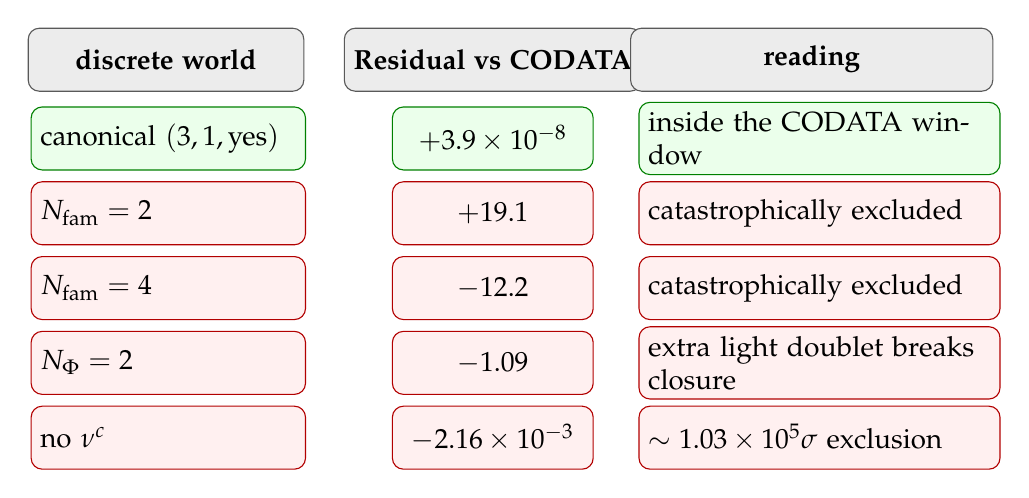
\begin{tikzpicture}[
    >=Latex,
    head/.style={draw=black!65, fill=gray!15, rounded corners, minimum height=0.8cm, align=center, font=\bfseries},
    ok/.style={draw=green!50!black, fill=green!8, rounded corners, minimum height=0.8cm, align=left},
    bad/.style={draw=red!70!black, fill=red!6, rounded corners, minimum height=0.8cm, align=left}
]
\node[head, minimum width=3.5cm] at (0,0) {discrete world};
\node[head, minimum width=2.8cm] at (4.15,0) {Residual vs CODATA};
\node[head, minimum width=4.6cm] at (8.2,0) {reading};

\node[ok, anchor=west, text width=3.25cm] at (-1.72,-1.0) {canonical $(3,1,\mathrm{yes})$};
\node[ok, minimum width=2.55cm] at (4.15,-1.0) {$+\num{3.9e-8}$};
\node[ok, anchor=west, text width=4.35cm] at (6.0,-1.0) {inside the CODATA window};

\node[bad, anchor=west, text width=3.25cm] at (-1.72,-1.95) {$N_{\mathrm{fam}}=2$};
\node[bad, minimum width=2.55cm] at (4.15,-1.95) {$+19.1$};
\node[bad, anchor=west, text width=4.35cm] at (6.0,-1.95) {catastrophically excluded};

\node[bad, anchor=west, text width=3.25cm] at (-1.72,-2.9) {$N_{\mathrm{fam}}=4$};
\node[bad, minimum width=2.55cm] at (4.15,-2.9) {$-12.2$};
\node[bad, anchor=west, text width=4.35cm] at (6.0,-2.9) {catastrophically excluded};

\node[bad, anchor=west, text width=3.25cm] at (-1.72,-3.85) {$N_\Phi=2$};
\node[bad, minimum width=2.55cm] at (4.15,-3.85) {$-1.09$};
\node[bad, anchor=west, text width=4.35cm] at (6.0,-3.85) {extra light doublet breaks closure};

\node[bad, anchor=west, text width=3.25cm] at (-1.72,-4.8) {no $\nu^c$};
\node[bad, minimum width=2.55cm] at (4.15,-4.8) {$-\num{2.16e-3}$};
\node[bad, anchor=west, text width=4.35cm] at (6.0,-4.8) {$\sim\num{1.03e5}\sigma$ exclusion};
\end{tikzpicture}
\caption{Exclusion matrix for wrong discrete worlds. The middle column records the residual versus the CODATA benchmark rather than a misleading shift relative to the canonical row. Once the discrete packet is changed, the electromagnetic closure leaves the observed window decisively.}
\label{fig:carrier-exclusion-matrix}
\end{figure}

\section{Closure architecture A: families, Higgs, and local spectral scale}

This first closure-architecture block is the shortest route from the hard carrier packet to a broader Standard Model plus gravity compiler. It has three moves: the local patch-deficit count gives the carrier-side family count, the topological family closure globalizes it into the family space $F$, the bosonic relative index selects the unique light Higgs doublet, and the local spectral-scale channel generates both $\Mpl$ and the electroweak vacuum from one common geometric response.

\subsection{Family monodromy and occupancy}

\begin{definition}[Family space]
Let $X_f$ denote the fundamental section of the seam complement. Define
\[
F:=H^1(X_f,\mathbb C).
\]
We use the distinguished cycle basis $(C_1,C_2,C_T)$ only as a concrete carrier-side basis of this family space; any later APS/Hodge realization is read as compatible analytic structure on the same topological family space.
\end{definition}
In this interpretation $F$ is neither an arbitrary flavor vector space nor a loose bookkeeping trick; it is a cycle space attached to the seam data. The actual bridge logic is shown in \Cref{fig:family-triangle}: the local patch-deficit count fixes $N_{\mathrm{fam}}=3$, the topological family step promotes that count to a family space, and the occupancy reinterpretation then feeds back into the defect channel.

\begin{figure}[t]
\centering
\scriptsize
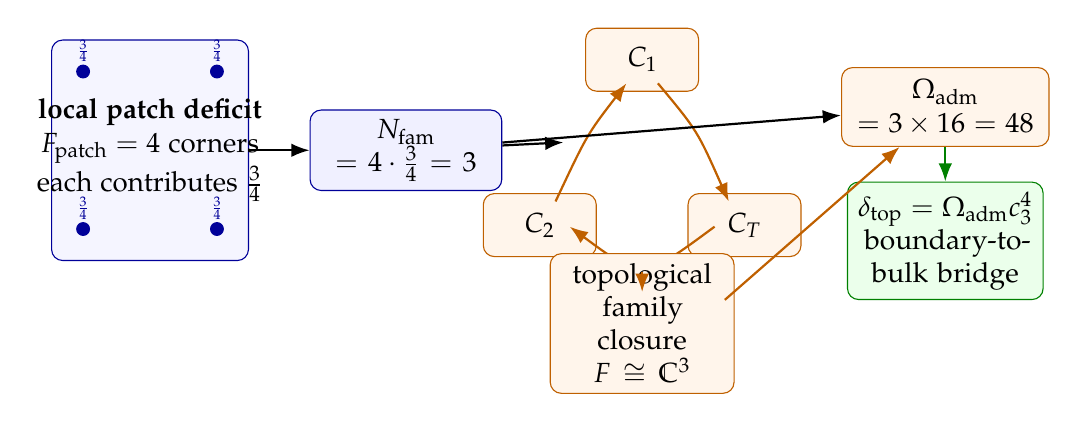
\begin{tikzpicture}[
    >=Latex,
    hard/.style={draw=blue!60!black, fill=blue!6, rounded corners, align=center, text width=2.2cm, minimum height=1.0cm},
    closure/.style={draw=orange!75!black, fill=orange!8, rounded corners, align=center, text width=2.4cm, minimum height=1.0cm},
    bridge/.style={draw=green!50!black, fill=green!8, rounded corners, align=center, text width=2.25cm, minimum height=1.0cm}
]
\draw[draw=blue!60!black, fill=blue!4, rounded corners] (-5.5,-1.4) rectangle (-3.0,1.4);
\foreach \x/\y in {-5.1/1.0,-3.4/1.0,-5.1/-1.0,-3.4/-1.0} {
    \filldraw[blue!60!black] (\x,\y) circle (2.3pt);
    \node[blue!60!black, anchor=south] at (\x,\y) {\tiny $\frac34$};
}
\node[align=center] at (-4.25,0) {\textbf{local patch deficit}\\$F_{\mathrm{patch}}=4$ corners\\each contributes $\frac34$};

\node[hard] (nfam) at (-1.0,0) {$N_{\mathrm{fam}}$\\$=4\cdot\frac34=3$};

\coordinate (A) at (2.0,1.15);
\coordinate (B) at (0.7,-0.95);
\coordinate (C) at (3.3,-0.95);
\node[closure, text width=1.2cm, minimum height=0.8cm] at (A) {$C_1$};
\node[closure, text width=1.2cm, minimum height=0.8cm] at (B) {$C_2$};
\node[closure, text width=1.2cm, minimum height=0.8cm] at (C) {$C_T$};
\draw[->, thick, orange!75!black] ($(A)+(0.2,-0.3)$) .. controls (2.7,0.25) .. ($(C)+(-0.2,0.3)$);
\draw[->, thick, orange!75!black] ($(C)+(-0.38,-0.02)$) .. controls (2.0,-1.65) .. ($(B)+(0.38,-0.02)$);
\draw[->, thick, orange!75!black] ($(B)+(0.2,0.3)$) .. controls (1.3,0.2) .. ($(A)+(-0.2,-0.3)$);
\node[closure, text width=2.1cm, minimum height=0.9cm] at (2.0,-2.2) {topological family closure\\$F\cong\mathbb C^3$};

\node[closure] (occ) at (5.85,0.55) {$\Omega_{\mathrm{adm}}$\\$=3\times16=48$};
\node[bridge] (dtop) at (5.85,-1.15) {$\deltatop=\Omega_{\mathrm{adm}}\cthree^4$\\boundary-to-bulk bridge};

\draw[->, thick] (-3.0,0) -- (nfam);
\draw[->, thick] (nfam) -- (1.0,0.1);
\draw[->, thick] (nfam) -- (occ);
\draw[->, thick, orange!75!black] (2.0,-1.55) -- (2.0,-1.8);
\draw[->, thick, orange!75!black] (3.05,-1.9) -- (occ);
\draw[->, thick, green!50!black] (occ) -- (dtop);
\end{tikzpicture}
\caption{Carrier-to-family closure bridge. The local patch-deficit count gives the hard multiplicity $N_{\mathrm{fam}}=3$, the topological family step turns that multiplicity into a genuine family space, and the resulting occupancy $\Omega_{\mathrm{adm}}=48$ feeds back into the defect reading $\deltatop=\Omega_{\mathrm{adm}}\cthree^4$.}
\label{fig:family-triangle}
\end{figure}

The Hodge metric on $F$ turns the monodromy data into an honest unitary family system rather than a merely decorative triangle sketch.

\begin{theorem}[Topological family closure on the orbifold seam section]
\label{thm:topological-family-closure}
\label{thm:orbifold-aps-family-master}
Let $X_f$ be the orbifold seam section with four $\mathbb Z_4$ corners. Then
\[
\chi_{\mathrm{orb}}(X_f)=1-4\left(1-\frac14\right)=-2,
\qquad
\rank H^{\mathrm{free}}_1(X_f,\mathbb Z)=3.
\]
Hence
\[
F:=H^1(X_f,\mathbb C)\cong \mathbb C^3,
\qquad
N_{\mathrm{fam}}=3,
\qquad
\Oadm=N_{\mathrm{fam}}\dim S^+=3\cdot 16=48.
\]
Equivalently, the local patch-deficit count is
\[
N_{\mathrm{fam}}=F_{\mathrm{patch}}\!\left(1-\frac14\right)=4\cdot\frac34=3.
\]
\end{theorem}

\begin{remark}[How the family theorem is now used]
The family theorem is used at topological strength in the present version. Any orbifold APS
realization is read as compatible analytic structure on the same closure, not as an additional
main-text theorem burden.
\end{remark}

\begin{proposition}[Orbifold APS compatibility]
\label{prop:orbifold-aps-compatibility}
Under the additional analytical hypotheses of \Cref{app:aps},
\[
\Ind^{\mathrm{orb,APS}}(D_{\mathrm{rel}}^+\otimes L_F)=3.
\]
\end{proposition}

\begin{corollary}[Boundary-to-bulk bridge corollary for the admissible occupancy]
\label{cor:boundary-bulk-occupancy}
On the canonical branch,
\[
\dim(S^+\otimes F)=16\cdot 3=48=\Oadm.
\]
Hence the topological surcharge enters the present paper as a derived occupancy corollary with an
observation-facing reading:
\[
\deltatop
=
\cthree^4\,\dim(S^+\otimes F)
=
\Oadm\,\cthree^4.
\]
\end{corollary}

The family subsection is therefore no longer split between a local count, an independent index theorem, and a later occupancy reinterpretation. Those statements are compressed into one topological theorem with one bridge corollary, while the holonomy proposition below records the resulting unitary geometry on $F$.

This theorem is the family statement referenced later by the admissibility theorems: the closure layer uses it as the explicit family component of the master closure theorem rather than as an external import.

\begin{proposition}[Special unitary family holonomy on the determinant-trivial branch]
\label{prop:family-holonomy-su3}
Let $L_F\to X_f$ be the flat Hermitian family bundle with fiber
$F\cong H^1(X_f,\mathbb C)$. Assume that its determinant line is flat trivial,
\[
\det L_F \cong X_f\times \mathbb C,
\]
and that the chosen flat connection preserves this trivialization. Then
\[
\mathrm{Hol}(\nabla_F)\subset SU(3)_F.
\]
\end{proposition}

\begin{proof}
The Hermitian metric implies
\[
\mathrm{Hol}(\nabla_F)\subset U(3).
\]
The induced connection on $\det L_F$ has trivial holonomy by assumption, so for
every loop $\gamma$ one has
\[
\det \rho_F(\gamma)=1.
\]
Hence every holonomy matrix lies in $SU(3)$.
\end{proof}

The role of the present subsection is thus no longer only mnemonic. It displays both the local patch-deficit count and the global APS/Hodge realization before the later closure stack compresses them into the theorem-level compiler surface.

\subsection{Occupancy and boundary-to-bulk bridge}

With the family bridge installed, the matter space becomes $S^+\otimes F$ and the occupancy $\Oadm=48$ is already fixed by the topological family theorem and its bridge corollary. Here \emph{occupancy} means the admissible chiral-state count after family lifting; it is not used as a primitive datum. The bridge point is not that family lifting creates a new numerical surcharge. Rather, the inherited hard kernel value
\[
\deltatop=\frac{3}{256\pi^4}
\]
admits on the canonical family branch the occupancy reinterpretation $\deltatop=\Oadm\,\cthree^4$.
Likewise the hard second-order defect contribution is re-read as
\[
\delta_2=\frac54\,\deltatop^2=B\gamma\,\Oadm^2\cthree^8.
\]
In the present manuscript this occupancy corollary is used with an observation-facing reading:
it is the boundary-to-bulk step that later feeds both the electromagnetic closure and the
geometric channel. The coefficient $5/4$ is therefore not an extra numerical motif; it is the
minimal-carrier compression factor $B\gamma$ rewritten in defect language. At the same time, the
equality $\deltatop=\Oadm\cthree^4$ is not presented as an independent dynamical transgression
theorem in the ordinary field-theory sense.

\subsection{From bridge to geometric completion}

\begin{principle}[Closure split]
Once the carrier packet and family closure architecture are fixed, the focused main-text closure
problem splits into a geometric program $\Ageom$ and a transport program $\Atrans$. Record
algebra and prediction semantics are now tied directly to the admissible gap in the main theorem
stack, while E$_8$ scale grammar and horizon extrapolations are deferred to appendix-level
continuations.
\end{principle}

\[
D_{\mathrm{geo}}:=D_{\mathrm{ref}}+D_{\mathrm{rel}}=D.
\]
The two main-text programs are packaged as
\[
\Ageom
:=
\langle E_3\oplus E_2,\ D_{\mathrm{geo}},\ \mathcal B_{\mathrm{rel}},\ \wspin\rangle,
\qquad
\Atrans
:=
\langle U_6,\ T,\ D_y,\ \mathcal Y_y^{(\varepsilon)},\ \mathcal C_{\Seam}\rangle.
\]
This split keeps the carrier theorem, the geometric reconstruction problem, and the record-level extensions from being flattened into one undifferentiated claim. In particular, the metric field is no longer treated here as an independent entry of $\Ageom$; it is reconstructed from the geometric Dirac anchor introduced next, while $D_{\mathrm{rel}}$ remains the comparison operator for spectral subtraction.

\subsection{Relative APS and superconnection setup}

The geometric completion is formulated on a graded bundle
\[
\mathcal E_{\mathrm{rel}}=\mathcal E_{\mathrm{rel}}^+\oplus\mathcal E_{\mathrm{rel}}^-,
\]
with the geometric Dirac anchor $D_{\mathrm{geo}}$, the declared reference operator
$D_{\mathrm{ref}}$, and APS-type boundary conditions on the seam $\Seam$; see
Appendix~\ref{app:aps}. The geometric package is
\[
\mathbb A_{\Seam}:=(D_{\mathrm{geo}},D_{\mathrm{rel}},A_{\Sigma}^{\mathrm{geo}}),
\qquad
A_{\Sigma}^{\mathrm{geo}}:=\mathcal B_{\mathrm{rel}}\oplus\nabla_{\chigeo}.
\]
Here $D_{\mathrm{geo}}$ is the geometric Dirac anchor, while $D_{\mathrm{rel}}$ is the relative comparison operator entering the spectral subtraction formulas. The bundle data $A_{\Sigma}^{\mathrm{geo}}$ reorganize the primitive seed package $A_{\Sigma}^{\mathrm{seed}}$ introduced earlier in \Cref{eq:tfpt-master}.
\begin{theorem}[Geometric reconstruction from the Dirac anchor]
\label{thm:geometric-reconstruction-anchor}
\label{thm:geometric-reconstruction-from-Dgeo}
\label{thm:relative-geometric-reconstruction}
Assume
\[
Z(\mathcal A)\cong C^\infty(M),
\]
and the geometric anchor $D_{\mathrm{geo}}$ is of Dirac type with principal symbol
\[
\sigma(D_{\mathrm{geo}})(x,\xi)^2
=
g^{\mu\nu}(x)\xi_\mu\xi_\nu\,\mathbf 1.
\]
Then $D_{\mathrm{geo}}$ reconstructs the metric $g$, the spin structure, and the
Levi--Civita connection on the geometric branch. Inner fluctuations of the same anchored
spectral datum generate the gauge sector.
The operator $D_{\mathrm{rel}}$ is the reference-subtracted comparison operator on that
same branch and is not itself used as the local geometric anchor.
\end{theorem}

\begin{proof}[Proof sketch]
On the admissible branch the commutative center identifies the manifold algebra, while the
principal symbol of the Dirac anchor determines the quadratic form on cotangent vectors.
Standard Dirac-type reconstruction then recovers the spin bundle and Levi--Civita connection
from that same symbol data. The relative operator changes the comparison bookkeeping, not the
geometric source of the local symbol.
\end{proof}

\begin{theorem}[Retained branch from the admissibility selector]
\label{thm:retained-branch-from-Padm}
\label{thm:admissible-sector-on-reconstructed-geometry}
\label{thm:full-operator-reconstruction}
Let $D_{\mathrm{geo}}$ be the geometric anchor and let $\Padm$ be the retained
admissibility selector.
Then:
\begin{enumerate}[label=(\roman*), leftmargin=1.5em, topsep=3pt, itemsep=2pt]
\item $X=\mathrm{Spec}\,Z(\mathcal A)$ and $\Seam=\mathrm{Fix}(\inv)$;
\item the local spectral density of $D_{\mathrm{geo}}$ determines the geometric response
      $\chigeo$;
\item $\Padm$ defines the retained admissible sector for observables, transport,
      and positivity statements on that branch.
\end{enumerate}
No claim is made that the compressed operator $\Padm D_{\mathrm{rel}}\Padm$
carries the local principal symbol of the geometry.
\end{theorem}

\begin{corollary}[No residual geometric datum beyond the geometric anchor]
The geometric package is reconstructed from $D_{\mathrm{geo}}$ and its local spectral density.
The selector $\Padm$ acts downstream on the retained sector and is not part of the
local geometric anchor.
\end{corollary}

\begin{definition}[Local spectral scale]
\label{def:local-spectral-scale}
Write the geometric response as a local spectral scale
\[
\chigeo=\Lambda e^\sigma,
\qquad
D_{\sigma,\mathrm{geo}}:=e^{-\sigma/2}D_{\mathrm{geo}}e^{-\sigma/2}.
\]
The relative spectral action is then organized as
\[
S_{\mathrm{rel}}[\sigma,D]
:=
\tr f\!\left(\frac{D_{\sigma,\mathrm{geo}}+\mathcal B_{\mathrm{rel}}}{\Lambda}\right)
-\tr f\!\left(\frac{D_{\mathrm{ref}}}{\Lambda}\right)
+\frac{i\pi}{2}\Delta\eta_\Sigma.
\]
\end{definition}

\begin{corollary}[Constant-scale reduction of the geometric branch]
\label{cor:constant-scale-reduction}
If the local spectral scale is frozen to a constant $\sigma=\sigma_0$, then $\chigeo=\chigeozero:=\Lambda e^{\sigma_0}$ and the present geometric branch reduces to the constant-$\chigeo$ closure relations
\[
\Mpl^2=\frac{\chigeozero^2}{2\pi^2},
\qquad
\vgeo^2=Z_H\,\frac{\mu_\Phi^2(\chigeozero)}{\lambda_\Phi}.
\]
Thus the former constant-$\chigeo$ formulas are retained as the homogeneous branch of the local spectral-scale formulation rather than as a competing package.
\end{corollary}


\subsection{Bosonic relative index and Higgs selection}

\begin{theorem}[Carrier-forced determinant classes on the seam]
\label{thm:determinant-class-higgs-selection}
Let
\[
L_2:=\det E_2,
\qquad
L_3:=\det E_3.
\]
Assume the total seam twist on the oriented double cover is one unit. Then the determinant holonomy classes satisfy
\[
[\mathrm{Hol}_\Sigma(L_2)]=1\in\pi_1(U(1)),
\qquad
[\mathrm{Hol}_\Sigma(L_3)]=0.
\]
Equivalently, for the asymptotic bosonic mass fields on the retained branch,
\[
\mathrm{wind}(\det\Phi_2)=1,
\qquad
\mathrm{wind}(\det\Phi_3)=0.
\]
The doublet winding is forced by the spin lift on the double cover, whereas center neutrality on the admissible branch forces determinant triviality in the triplet sector.
\end{theorem}

\begin{proof}[Proof sketch]
The oriented double cover already forces a half-angle lift on the rank-two weak sector. Passing to the determinant line therefore gives one full winding in $L_2$. By contrast, the admissible branch requires center neutrality in the color sector, so the determinant line of $E_3$ is trivial on the retained branch. One unit of total seam twist can therefore be realized only by the doublet determinant class.
\end{proof}

\begin{remark}[Energy interpretation on the retained branch]
The older asymptotic bosonic functional
\[
\mathcal E_{\mathrm{asym}}(\Phi_2,\Phi_3)
:=
\tau_2\bigl|\mathrm{wind}(\det\Phi_2)\bigr|
+\tau_3\bigl|\mathrm{wind}(\det\Phi_3)\bigr|
+m_3^2\dim\ker\mathcal B_{E_3}^+,
\]
with $\tau_3>\tau_2>0$, remains a useful physical intuition for why the retained branch is energetically preferred. In the present rewrite, however, the structural weight is carried by the determinant-class theorem above rather than by the cost functional itself.
\end{remark}

\begin{theorem}[Callias Higgs selection from determinant classes]
\label{thm:callias-higgs-selection}
Let $N_\Seam$ be the oriented two-dimensional normal slice to the seam. For $a\in\{2,3\}$ define
\[
\mathcal B_{E_a}:=\sigma^\mu\nabla^{(a)}_\mu+\Phi_a
\]
on $N_\Seam$, where $\Phi_a$ is asymptotically invertible on the boundary at infinity. Under the determinant-class data of \Cref{thm:determinant-class-higgs-selection}, assume
\[
(\mathcal B_{E_2}^-)^\dagger\mathcal B_{E_2}^-\ge m_-^2>0,
\qquad
(\mathcal B_{E_3}^{\pm})^\dagger\mathcal B_{E_3}^{\pm}\ge m_3^2>0.
\]
Then the bosonic relative index satisfies
\[
\Ind_{\mathrm{rel}}^{\Padm}(\mathcal B_{E_2}^+)=1,
\qquad
\Ind_{\mathrm{rel}}^{\Padm}(\mathcal B_{E_3}^+)=0.
\]
Moreover,
\[
\dim\ker\mathcal B_{E_2}^+=1,
\qquad
\ker\mathcal B_{E_2}^-=\ker\mathcal B_{E_3}^{\pm}=0.
\]
Consequently the unique light seam-even bosonic zero mode lies in
\[
\Phi\in\Gamma(E_2)\cong (1,2)_{1/2},
\qquad
\inv\Phi=+\Phi.
\]
\end{theorem}

\begin{proof}[Proof sketch]
By \Cref{thm:determinant-class-higgs-selection}, the retained branch fixes the asymptotic winding data to
\[
\mathrm{wind}(\det\Phi_2)=1,
\qquad
\mathrm{wind}(\det\Phi_3)=0.
\]
The Callias index theorem then gives
\[
\Ind_{\mathrm{rel}}^{\Padm}(\mathcal B_{E_2}^+)=1,
\qquad
\Ind_{\mathrm{rel}}^{\Padm}(\mathcal B_{E_3}^+)=0.
\]
The positivity bounds remove the opposite chirality and all triplet zero modes, so the index lifts to an actual uniqueness statement for one seam-even Higgs doublet.
\end{proof}

This is the sharp form of the Higgs claim used here. The issue is not whether a Higgs doublet can be written down, but whether the relative bosonic index can be shown to select it uniquely.
Without a genuine Callias / Dirac / Dolbeault-type index problem there would be no mathematical reason for one light doublet and no light triplet to emerge from the bosonic sector. Once that uniqueness statement is fixed, the renormalizable carrier-compatible Yukawa couplings are the standard ones,
\[
Q\,u^c\,\Phi,
\qquad
Q\,d^c\,\Phi^\dagger,
\qquad
L\,e^c\,\Phi^\dagger,
\qquad
L\,\nu^c\,\Phi,
\]
so the Higgs statement becomes a genuine structural bridge rather than a notation choice.

\subsection{Heat-kernel coefficient map and local spectral-scale bifurcation}

The local target action is written as
\begin{equation}
\label{eq:chi-effective-action}
\begin{aligned}
\Gammaeff
=
\int d^4x\sqrt{-g}\,
\Big[
c_R\chigeo^2R
+Z_\chi(\partial\chigeo)^2
-\mu_\Phi^2(\chigeo)\,\Phi^\dagger\Phi
+\lambda_\Phi(\Phi^\dagger\Phi)^2
+\frac{1}{6M^2}R^2
+\cdots
\Big].
\end{aligned}
\end{equation}
The relative bosonic endomorphism used below is
\begin{equation}
\label{eq:relative-bosonic-endomorphism}
E_{\mathrm{rel}}
=
-\frac14 R\,\mathbf 1_{48}
-
(\Phi^\dagger\Phi)\,P_2
+
\frac12\gamma^{\mu\nu}\mathbb F_{\mu\nu},
\end{equation}
and the coefficient bookkeeping expected from the relative spectral expansion is summarized in \Cref{tab:heat-kernel-map}.

\begin{table}[t]
\centering
\small
\begin{tabularx}{\linewidth}{@{}>{\raggedright\arraybackslash}p{0.15\linewidth}>{\raggedright\arraybackslash}p{0.22\linewidth}>{\raggedright\arraybackslash}p{0.22\linewidth}>{\raggedright\arraybackslash}p{0.14\linewidth}>{\raggedright\arraybackslash}p{0.14\linewidth}@{}}
\toprule
Coefficient & Operator sector & Generated term & $\chigeo$ scaling & Status \\
\midrule
$a_0$ & relative bulk trace & vacuum-energy bookkeeping & $\chigeo^4$ & Hard \\
$a_2$ & seam-even bosonic bulk term & $\chigeo^2R$, $\chigeo^2\Phi^\dagger\Phi$ & $\chigeo^2$ & Closure \\
$a_4$ & local bosonic sector & $|D\Phi|^2$, $(\Phi^\dagger\Phi)^2$, $R\,\Phi^\dagger\Phi$, $\tr\mathbb F^2$, $R^2$ & $\chigeo^0$ & Closure \\
boundary/defect term & seam correction and parity data & local defect counterterms, seam-even selection & $\Delta_{\Seam}$ & Closure \\
$\eta$ term & APS spectral asymmetry & sign and spectral-flow control & scale free & Closure \\
\bottomrule
\end{tabularx}
\caption{Heat-kernel map for the geometric closure architecture.}
\label{tab:heat-kernel-map}
\end{table}

The resulting geometric logic is displayed in \Cref{fig:chi-bifurcation}. The same coefficient map controls the Einstein term, the Higgs normalization, the Higgs vacuum relation, and the curvature/gauge side terms. This is why the local spectral-scale sector is the principal geometric closure channel of the manuscript rather than just one more scalar parameter.

\begin{figure}[t]
\centering
\scriptsize
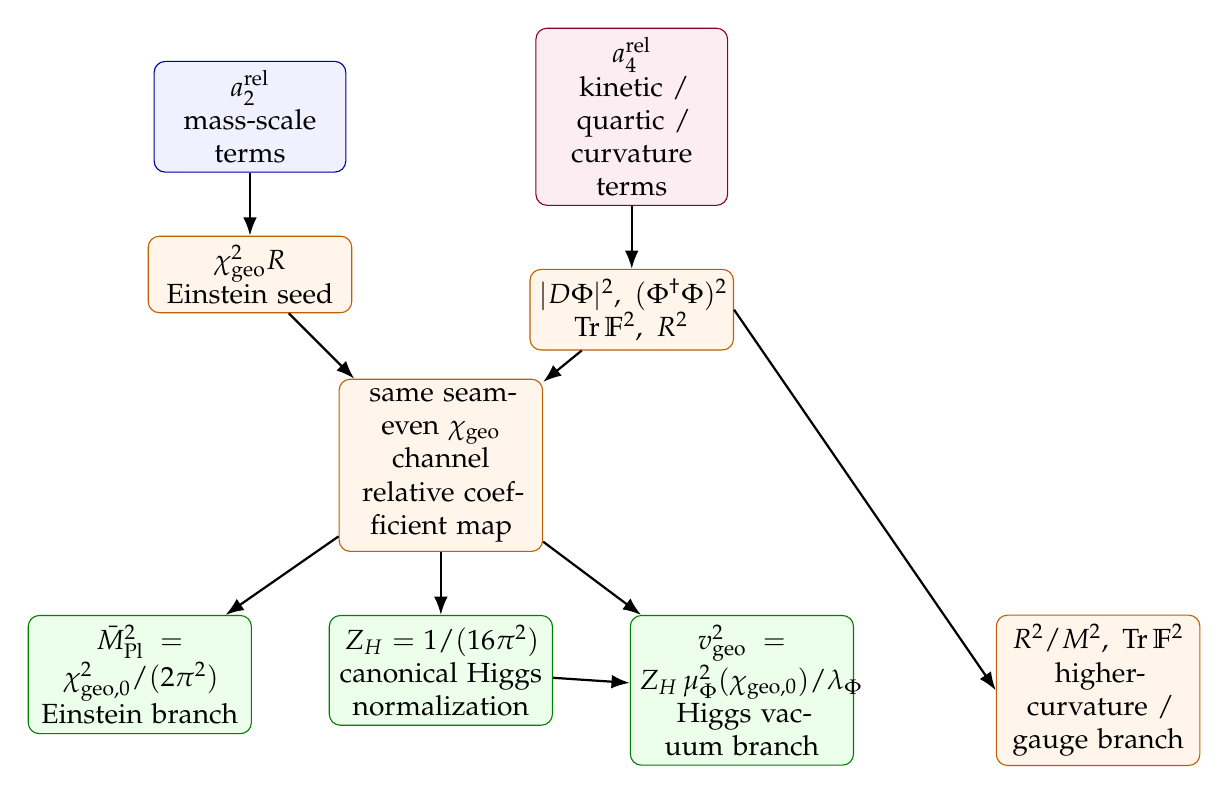
\begin{tikzpicture}[
    >=Latex,
    node distance=8mm and 11mm,
    a2/.style={draw=blue!60!black, fill=blue!6, rounded corners, align=center, text width=2.2cm, minimum height=0.9cm},
    a4/.style={draw=purple!70!black, fill=purple!7, rounded corners, align=center, text width=2.2cm, minimum height=0.9cm},
    flow/.style={draw=orange!75!black, fill=orange!8, rounded corners, align=center, text width=2.35cm, minimum height=0.95cm},
    outbox/.style={draw=green!50!black, fill=green!8, rounded corners, align=center, text width=2.6cm, minimum height=0.95cm}
]
\node[a2] (a2node) {$a_2^{\mathrm{rel}}$\\mass-scale terms};
\node[a4, right=24mm of a2node] (a4node) {$a_4^{\mathrm{rel}}$\\kinetic / quartic / curvature terms};

\node[flow, below=of a2node] (ein0) {$\chigeo^2R$\\Einstein seed};
\node[flow, below=of a4node] (kin0) {$|D\Phi|^2,\ (\Phi^\dagger\Phi)^2$\\$\tr\mathbb F^2,\ R^2$};
\node[flow, below=of $(ein0)!0.5!(kin0)$, yshift=-3mm] (chi) {same seam-even $\chigeo$ channel\\relative coefficient map};

\node[outbox, below left=of chi] (mpl) {$\Mpl^2=\chigeozero^2/(2\pi^2)$\\Einstein branch};
\node[outbox, below=of chi] (zh) {$Z_H=1/(16\pi^2)$\\canonical Higgs normalization};
\node[outbox, below right=of chi] (vev) {$\vgeo^2=Z_H\,\mu_\Phi^2(\chigeozero)/\lambda_\Phi$\\Higgs vacuum branch};
\node[flow, right=18mm of vev] (curv) {$R^2/M^2,\ \tr\mathbb F^2$\\higher-curvature / gauge branch};

\draw[->, thick] (a2node) -- (ein0);
\draw[->, thick] (a4node) -- (kin0);
\draw[->, thick] (ein0) -- (chi);
\draw[->, thick] (kin0) -- (chi);
\draw[->, thick] (chi) -- (mpl);
\draw[->, thick] (chi) -- (zh);
\draw[->, thick] (chi) -- (vev);
\draw[->, thick] (kin0.east) -- (curv.west);
\draw[->, thick] (zh) -- (vev);
\end{tikzpicture}
\caption{Coefficient flow of the local spectral-scale channel. The $a_2$ coefficient supplies the Einstein and Higgs mass seeds, the $a_4$ coefficient supplies kinetic/quartic/gauge-curvature data, and the same seam-even $\chigeo$ response turns both streams into the coupled relations for $\Mpl$ and $\vgeo$.}
\label{fig:chi-bifurcation}
\end{figure}

\begin{proposition}[Canonical bosonic normalization on the seam-even branch]
\label{prop:canonical-bosonic-normalization}
On the seam-even bosonic branch selected by $P_2$, the relative Seeley--DeWitt map is
\begin{equation}
\label{eq:relative-a2}
\begin{aligned}
a_2^{\mathrm{rel}}
=
-\int d^4x\sqrt g
\left(
\frac{\chigeo^2}{4\pi^2}R
+
\frac{\chigeo^2}{8\pi^2}\Phi^\dagger\Phi
\right)
+
a_{2,\Seam},
\end{aligned}
\end{equation}
\begin{equation}
\label{eq:relative-a4}
\begin{aligned}
a_{4,\mathrm{rel}}
=
\int d^4x\sqrt g
\left[
\frac{1}{16\pi^2}|D\Phi|^2
+
\frac{1}{16\pi^2}(\Phi^\dagger\Phi)^2
+
\frac{1}{96\pi^2}R\,\Phi^\dagger\Phi
+
\frac{1}{192\pi^2}\tr\mathbb F^2
+\dots
\right]
+
a_{4,\Seam}.
\end{aligned}
\end{equation}
Therefore the bosonic normalization constants are
\[
\Mpl^2=\frac{\chigeozero^2}{2\pi^2},
\qquad
Z_H=\frac{1}{16\pi^2},
\qquad
\Phi_{\mathrm{can}}:=\sqrt{Z_H}\,\Phi=\frac{\Phi}{4\pi},
\]
and the canonical Higgs vacuum relation becomes
\begin{equation}
\label{eq:induced-einstein}
\Mpl^2=\frac{\chigeozero^2}{2\pi^2},
\qquad
\vgeo^2=Z_H\,\frac{\mu_\Phi^2(\chigeozero)}{\lambda_\Phi}.
\end{equation}
\end{proposition}

\begin{proof}[Proof sketch]
The operator \Cref{eq:relative-bosonic-endomorphism} is the seam-even bosonic endomorphism entering the relative heat-kernel expansion. The $a_2$ coefficient fixes the Einstein branch and the bosonic mass term, while $a_4$ fixes the scalar kinetic normalization, quartic coefficient, mixed curvature term, and gauge curvature trace. The coefficient of $|D\Phi|^2$ is therefore the wave-function factor $Z_H=1/(16\pi^2)$. After the canonical rescaling $\Phi_{\mathrm{can}}=\sqrt{Z_H}\,\Phi$, the Einstein and Higgs branches are read from the same relative coefficient map rather than from separate normalization conventions.
\end{proof}

\begin{remark}[Newton form is not an independent output]
Using the standard reduced-Planck definition $\Mpl^{-2}=8\pi G_N$, the first relation in \Cref{eq:induced-einstein} is equivalently
\[
G_N\chigeozero^2=\frac{\pi}{4}.
\]
This Newton-form equation is therefore a rewriting of the Einstein-branch closure, not a second independent prediction.
\end{remark}

\begin{lemma}[Two-sheet seam-even zero-mode normalization]
\label{lem:two-sheet-zero-mode-normalization}
If the seam-even Higgs zero mode is normalized across both sheets of the oriented double cover, then its branch weight is
\[
w_H
=
2\,\gcar\,\beta_{\mathrm{rad}}^2
\exp\!\left[-\frac{\alpha^{-1}(0)+\delta_{\mathrm{ph}}}{5}\right].
\]
With
\[
\mu_\Phi^2(\chigeozero)=\frac{\chigeozero^2}{8\pi^2}w_H^2,
\qquad
\lambda_\Phi=\frac{1}{16\pi^2},
\]
the canonical Higgs vacuum expectation value is
\begin{equation}
\label{eq:carrier-dressed-v}
\vgeo
=
\Mpl\,\gcar\,\beta_{\mathrm{rad}}^2\,
\exp\!\left[-\frac{\alpha^{-1}(0)+\delta_{\mathrm{ph}}}{5}\right].
\end{equation}
\end{lemma}

\begin{proof}[Proof sketch]
The two-sheet seam-even normalization doubles the unnormalized zero-mode weight and therefore produces the stated $w_H$. Since the canonical Higgs field is $\Phi_{\mathrm{can}}=\sqrt{Z_H}\,\Phi$, its vacuum relation is
\[
\vgeo^2=\frac{Z_H\mu_\Phi^2(\chigeozero)}{\lambda_\Phi}
=
\frac{\chigeozero^2}{8\pi^2}w_H^2.
\]
Using $\Mpl^2=\chigeozero^2/(2\pi^2)$ from \Cref{prop:canonical-bosonic-normalization} gives $\vgeo=\Mpl w_H/2$, hence \Cref{eq:carrier-dressed-v}.
\end{proof}

\begin{remark}[Geometric versus benchmark electroweak scales]
For source formulas driven by the bosonic closure we write $\vgeo$ for the quantity in \Cref{eq:carrier-dressed-v}. Numerically,
\[
\vgeo\approx\num{241.87}\;\mathrm{GeV}.
\]
This is the internal geometric branch value used in the charged-lepton and seesaw source formulas. When the manuscript compares to the measured electroweak vacuum parameter at the benchmark interface, it instead uses
\[
\vewref:=\num{246.22}\;\mathrm{GeV},
\]
as an external reference value. These two numbers therefore belong to different bookkeeping layers and must not be silently interchanged inside one derivation or one table.
\end{remark}

\begin{remark}[Sector-dressed local spectral-scale channels]
The quantity $\chigeozero$ entering the induced Einstein channel is not identified with the transport-sector confinement scale. In the hadronic sector we write $\chi_{\QCD}$ and regard it as a locally dressed channel obtained from the same underlying primitive response $\chiseed$ after sector-dependent renormalization and confinement-scale matching:
\[
\chiseed \longrightarrow \chigeozero \quad \text{(gravitational background)},
\qquad
\chiseed \longrightarrow \chi_{\QCD} \quad \text{(transport-dressed local channel)}.
\]
This is the minimal statement needed to avoid the otherwise immediate scale clash between the Planck bridge and the QCD string tension.
\end{remark}

\begin{figure}[t]
\centering
\scriptsize
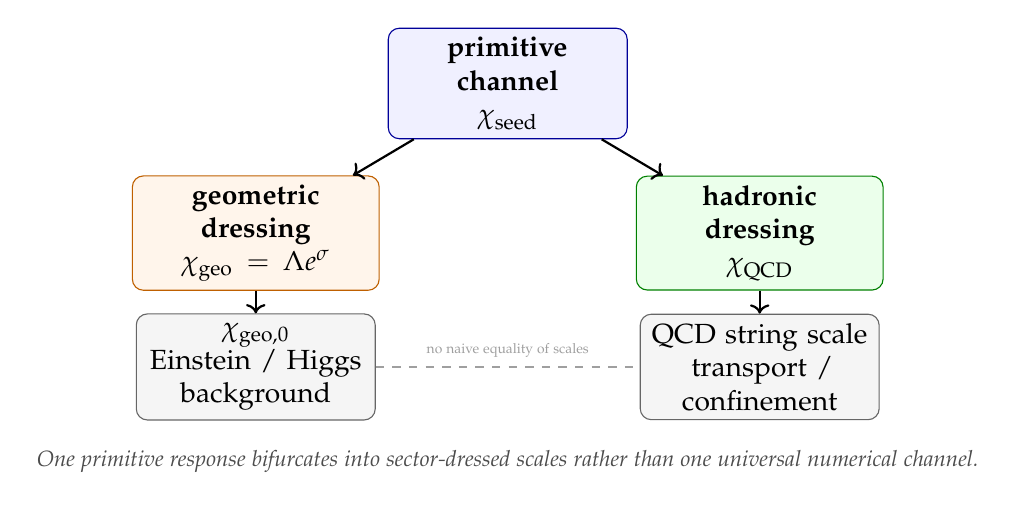
\begin{tikzpicture}[
    seed/.style={draw=blue!60!black, fill=blue!6, rounded corners, text width=2.8cm, minimum height=1.0cm, align=center},
    geo/.style={draw=orange!75!black, fill=orange!8, rounded corners, text width=2.9cm, minimum height=1.0cm, align=center},
    qcd/.style={draw=green!50!black, fill=green!8, rounded corners, text width=2.9cm, minimum height=1.0cm, align=center},
    result/.style={draw=black!60, fill=gray!8, rounded corners, text width=2.8cm, minimum height=0.95cm, align=center},
    note/.style={font=\footnotesize\itshape, text=black!70, align=center}
]
\node[seed] (seed) at (0,0) {\textbf{primitive channel}\\$\chiseed$};
\node[geo] (geo) at (-3.2,-1.9) {\textbf{geometric dressing}\\$\chigeo=\Lambda e^\sigma$};
\node[result] (geoz) at (-3.2,-3.6) {$\chigeozero$\\Einstein / Higgs background};
\node[qcd] (qcd) at (3.2,-1.9) {\textbf{hadronic dressing}\\$\chi_{\QCD}$};
\node[result] (had) at (3.2,-3.6) {QCD string scale\\transport / confinement};
\draw[->, thick] (seed) -- (geo);
\draw[->, thick] (geo) -- (geoz);
\draw[->, thick] (seed) -- (qcd);
\draw[->, thick] (qcd) -- (had);
\draw[dashed, gray!75] (geoz) -- node[above, sloped] {\tiny no naive equality of scales} (had);
\node[note] at (0,-4.8) {One primitive response bifurcates into sector-dressed scales rather than one universal numerical channel.};
\end{tikzpicture}
\caption{Local spectral-scale bifurcation. The primitive response $\chiseed$ is later dressed geometrically into $\chigeo$ and its vacuum branch $\chigeozero$, while the hadronic sector dresses the same primitive channel into $\chi_{\QCD}$. This is the clean separation that prevents the Planck/Higgs/QCD scale clash.}
\label{fig:chi-bifurcation-clean}
\end{figure}

\begin{theorem}[Relative spectral gravity branch]
\label{thm:gravity-cosmology-closure}
The same geometric closure sector defines a local spectral gravity branch of schematic form
\[
\Gamma_{\mathrm{grav}}
:=
\int d^4x\sqrt{-g}\Big[
\frac12 Z_N(\chigeo)\chigeo^2R
+\frac12 Z_\chi(\nabla\chigeo)^2
-U(\chigeo)
+R\,\mathcal F_R(\Box/\chigeo^2)R
+C\,\mathcal F_C(\Box/\chigeo^2)C
+|D\Phi|^2
-V(\Phi,\chigeo)
-\sum_a \frac{1}{4g_a^2}\tr F_{a,\mu\nu}F_a^{\mu\nu}
+\cdots
\Big].
\]
On the low-curvature local branch, the form factors reduce to the retained local coefficients and one recovers the effective action
\[
\Gamma_{\mathrm{grav}}^{\mathrm{eff}}
:=
\int d^4x\sqrt{-g}\Big[
\frac{\Mpl^2}{2}R
-\Lambda_{\Seam,\mathrm{ren}}
+\frac{1}{6M^2}R^2
+\frac{Z_\chi}{2}(\nabla\chigeo)^2
-U(\chigeo)
+|D\Phi|^2
-V(\Phi,\chigeo)
-\sum_a \frac{1}{4g_a^2}\tr F_{a,\mu\nu}F_a^{\mu\nu}
\Big],
\]
with
\[
\Mpl^2=\frac{\chigeozero^2}{2\pi^2},
\qquad
\vgeo^2=\frac{Z_H\mu_\Phi^2(\chigeozero)}{\lambda_\Phi}.
\]
Its low-curvature Euler--Lagrange equations are
\[
\Mpl^2 G_{\mu\nu}
+\Lambda_{\Seam,\mathrm{ren}} g_{\mu\nu}
+\frac{1}{3M^2}\mathcal H_{\mu\nu}
=
T_{\mu\nu}^{(\chigeo,\Phi,A,\psi)},
\]
\[
Z_\chi\Box\chigeo=U'(\chigeo)+\partial_{\chigeo}V(\Phi,\chigeo),
\qquad
D^\mu D_\mu\Phi=\partial_{\Phi^\dagger}V(\Phi,\chigeo),
\]
where
\[
\mathcal H_{\mu\nu}
:=
RR_{\mu\nu}
-\frac14 g_{\mu\nu}R^2
-\nabla_\mu\nabla_\nu R
+g_{\mu\nu}\Box R.
\]
On the low-curvature vacuum branch
\[
R\ll M^2,
\qquad
\chigeo=\chigeozero,
\qquad
\Phi=\frac{1}{\sqrt2}\binom{0}{\vgeo},
\]
the theory reduces to Einstein gravity with renormalized seam vacuum energy $\Lambda_{\Seam,\mathrm{ren}}$.
On the early-universe $R^2$ branch, the Einstein-frame scalaron potential is
\[
V_{\mathrm{sc}}(\varphi)
=
\frac34 M^2\Mpl^2
\left(1-e^{-\sqrt{2/3}\,\varphi/\Mpl}\right)^2
+\Lambda_{\Seam,\mathrm{ren}}.
\]
For spatially flat FRW one has
\[
3\Mpl^2\Hhub^2
=
\frac12\dot\varphi^2+V_{\mathrm{sc}}(\varphi)+\rho_m,
\qquad
\dot{\Hhub}
=
-\frac{1}{2\Mpl^2}\bigl(\dot\varphi^2+\rho_m+p_m\bigr),
\]
and the usual slow-roll observables
\[
A_s=\frac{V_*}{24\pi^2\Mpl^4\epsilon_*},
\qquad
n_s=1-6\epsilon_*+2\eta_*,
\qquad
r=16\epsilon_*.
\]
\end{theorem}

\begin{proof}[Proof sketch]
The $a_2$ and $a_4$ coefficient map of \Cref{eq:chi-effective-action,eq:relative-a2,eq:relative-a4}, together with the local spectral-scale formulation of \Cref{def:local-spectral-scale}, already contains the Einstein term, the Higgs sector, the $R^2$ branch, and the gauge-curvature sector in one seam-even closure package. The low-curvature limit freezes $\chigeo$ and $\Phi$ on the vacuum branch, while the higher-curvature terms reduce to the retained local $R^2$ approximation used here.
\end{proof}

\begin{corollary}[Classical limit]
On the vacuum branch the effective theory reproduces Einstein gravity with cosmological constant, Standard Model gauge fields, one seam-even Higgs doublet, and three chiral families.
\end{corollary}

\begin{theorem}[Conditional UV Bernstein-cone program]
\label{thm:uv-bernstein-cone-completion}
Assume the projected RG flow preserves the admissible Bernstein cone and admits a nontrivial UV
fixed point satisfying the pole and positivity audit below. The effective average action is
sought in the form
\[
\Gamma_k
=
\int d^4x\sqrt g\,
\Bigl[
\frac{M_k^2}{2}R
+C\,\mathcal F_{C,k}(\Box/\chigeo^2)\,C
+R\,\mathcal F_{R,k}(\Box/\chigeo^2)\,R
+\frac12 Z_{\chi,k}(\nabla\chigeo)^2
+U_k(\chigeo,\Phi)
+\cdots
\Bigr],
\]
where the sector form factors are constrained by complete Bernstein functions
\[
\Phi_{s,k}(z)
:=
a_{s,k}+b_{s,k}z+\int_0^\infty \frac{z}{u+z}\rho_{s,k}(u)\,du,
\qquad
\rho_{s,k}(u)\ge 0.
\]
The admissible RG flow is required to preserve both the retained sector and this
cone:
\[
\partial_t\Gamma_k
:=
\frac12\mathrm{STr}_{\Padm}
\Bigl[
\bigl(\Gamma_k^{(2)}+R_k\bigr)^{-1}\partial_t R_k
\Bigr],
\]
with regulator $R_k$ commuting with $\Padm$, $Q_\Theta$, and $\inv$ and living in
the same Bernstein class. Sectorwise the inverse propagators are then required to
take the form
\[
\Gamma^{(2)}_{2,k}(p^2)
=
Z_{N,k}\,p^2\,\Phi_{2,k}(p^2/\chigeo^2),
\]
\[
\Gamma^{(2)}_{0,k}(p^2)
=
Z_{0,k}\,(p^2+M_{s,k}^2)\,\Phi_{0,k}(p^2/\chigeo^2).
\]
The conditional UV program closes only if three conditions hold simultaneously:
\begin{enumerate}[label=(\roman*), leftmargin=1.5em, topsep=3pt, itemsep=2pt]
    \item the admissible Bernstein cone is invariant under the projected RG flow,
    \item the flow admits a nontrivial UV fixed point on that cone,
    \item and the pole/positivity audit closes on $\operatorname{Ran}(\Padm)$:
    exactly one massless spin-$2$ pole, exactly one healthy scalaron pole with
    $M_{s,k}^2>0$ and positive residue, no extra ghost/tachyon branches, and
    positive spectral density compatible with admissible reflection positivity.
\end{enumerate}
Under these assumptions, the projected RG flow preserves the admissible complete-Bernstein cone,
admits a nontrivial UV fixed point on the bounded moment body, and closes the pole/positivity
audit on $\operatorname{Ran}(\Padm)$ with exactly one massless spin-$2$ pole, exactly one
healthy scalaron pole, and no extra ghost or tachyon branches. The local Einstein plus $R^2$
branch is therefore interpreted as the infrared projection of an admissible UV Bernstein-cone
program.
\end{theorem}

\begin{theorem}[Conditional regulator equivalence inside the admissible Bernstein cone]
\label{thm:regulator-equivalence-bernstein-cone}
Assume the hypotheses of \Cref{thm:uv-bernstein-cone-completion}. Let $R_k$ and
$\widetilde R_k$ be two admissible projected regulators in the same complete Bernstein class,
both commuting with $\Padm$, $Q_\Theta$, and $\inv$, and both normalized to the same infrared
data. Then their induced admissible RG flows determine the same:
\begin{enumerate}[label=(\roman*), leftmargin=1.5em, topsep=3pt, itemsep=2pt]
    \item fixed-point pole data in the spin-$2$ and spin-$0$ sectors,
    \item number of relevant UV directions,
    \item infrared Einstein--$R^2$ closure class on the admissible branch.
\end{enumerate}
Hence the conditional UV program of \Cref{thm:uv-bernstein-cone-completion} is regulator
independent inside the admissible Bernstein-cone class.
\end{theorem}

The E$_8$ scale ladder is not used as a primitive input in the main text. Only its short downstream grammar is retained in the dedicated main-text section, while the fuller arithmetic continuations are deferred to Appendix~\ref{app:constants}.

\section{Closure architecture B: Yukawas, masses, flavor, confinement, and strong CP}

The second closure-architecture block is the transport compiler. Its role is to turn the carrier packet and the family/occupancy closure into actual masses, mixings, hadronic admissibility, and strong-CP control. The logic is again staged: first the discrete phase operator and the transport kernel, then path-length masses and mixing data, then confinement and strong CP as transport-side admissibility statements.

\subsection{Discrete phase operator and transport grammar}

Let
\[
\omega=e^{2\pi i/3},
\qquad
U_6=\mathrm{diag}(1,\omega,\omega^2,-1,-\omega,-\omega^2).
\]
This makes the phase grammar concrete rather than rhetorical. The six admissible phases are shown as a finite hexagonal transport geometry in \Cref{fig:z6-circle}: the cusp values live on the same real axis as the positive-real phase, the admissible gap is visible directly, and the holonomy phase can be read as a triangle on the same discrete transport base.

\begin{remark}[Hexagonal spectral geometry]
The operator $U_6$ is a unitary circulant with eigenphases $e^{in\pi/3}$ for $n=0,\dots,5$ and is unitarily equivalent to the one-step translation operator on a six-site ring. The transport kernel $D_y=y\,\mathbf 1-\delta_{\mathrm{ph}}U_6$ is therefore the resolvent denominator of a finite quantum walk, equivalently a tight-binding transfer problem, on the discrete $C_6$ cycle. The regularized inverse introduced below plays the role of the corresponding Green kernel. CKM and PMNS mixings, mass hierarchies, and the Möbius quotients of \Cref{eq:mobius-quotient} are thus not loose analytic fits but spectral-theory statements on a regular hexagon. The near-pole hierarchy at $y\approx\delta_{\mathrm{ph}}$ becomes the resonance of a hexagonal resolvent rather than tuned parameter choice.
\end{remark}

\begin{figure}[t]
\centering
\scriptsize
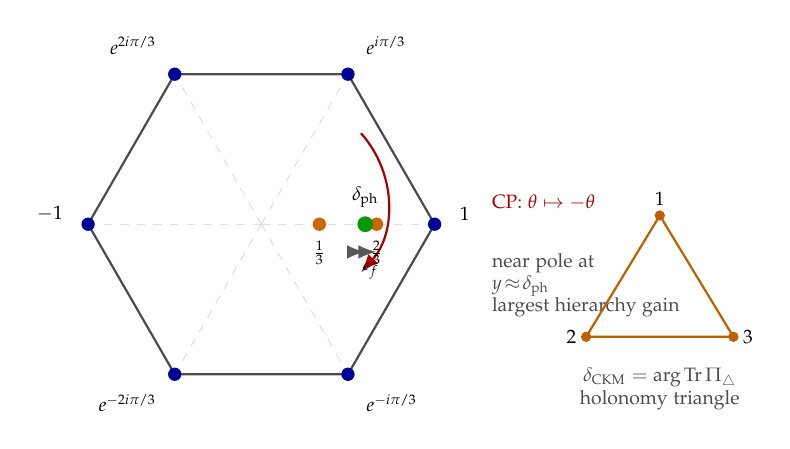
\begin{tikzpicture}[scale=1.1,>=Latex]
\coordinate (O) at (0,0);
\foreach \name/\ang in {p0/0,p1/60,p2/120,p3/180,p4/240,p5/300} {
    \coordinate (\name) at ({2*cos(\ang)},{2*sin(\ang)});
}
\draw[thick, black!70] (p0) -- (p1) -- (p2) -- (p3) -- (p4) -- (p5) -- cycle;
\draw[gray!25, dashed] (O) -- (p0);
\draw[gray!25, dashed] (O) -- (p1);
\draw[gray!25, dashed] (O) -- (p2);
\draw[gray!25, dashed] (O) -- (p3);
\draw[gray!25, dashed] (O) -- (p4);
\draw[gray!25, dashed] (O) -- (p5);
\foreach \P in {p0,p1,p2,p3,p4,p5} {
    \filldraw[blue!60!black] (\P) circle (2pt);
}
\node[anchor=west, font=\scriptsize] at (2.18,0.12) {$1$};
\node[anchor=south west, font=\scriptsize] at (1.1,1.85) {$e^{i\pi/3}$};
\node[anchor=south east, font=\scriptsize] at (-1.1,1.85) {$e^{2i\pi/3}$};
\node[anchor=east, font=\scriptsize] at (-2.18,0.12) {$-1$};
\node[anchor=north east, font=\scriptsize] at (-1.1,-1.85) {$e^{-2i\pi/3}$};
\node[anchor=north west, font=\scriptsize] at (1.1,-1.85) {$e^{-i\pi/3}$};

\draw[->, thick, red!65!black] (1.15,1.05) arc[start angle=42,end angle=-42,radius=1.2];
\node[red!65!black, font=\scriptsize, anchor=west] at (2.55,0.25) {CP: $\theta\mapsto-\theta$};

\filldraw[orange!80!black] (0.67,0) circle (2pt);
\filldraw[orange!80!black] (1.33,0) circle (2pt);
\filldraw[green!60!black] (1.1998,0) circle (2.4pt);
\node[below, font=\scriptsize] at (0.67,-0.08) {$\frac13$};
\node[below, font=\scriptsize] at (1.33,-0.08) {$\frac23$};
\node[above, font=\scriptsize] at (1.1998,0.08) {$\delta_{\mathrm{ph}}$};
\draw[<->, thick, black!65] (1.1998,-0.32) -- (1.33,-0.32);
\node[below, font=\tiny] at (1.265,-0.34) {$\epsilon_f$};
\node[align=left, anchor=west, font=\scriptsize, text=black!70] at (2.55,-0.7)
    {near pole at\\$y\!\approx\!\delta_{\mathrm{ph}}$\\largest hierarchy gain};

\begin{scope}[shift={(4.6,-0.8)}]
    \coordinate (A) at (0,0.9);
    \coordinate (B) at (-0.85,-0.5);
    \coordinate (C) at (0.85,-0.5);
    \draw[thick, orange!75!black] (A) -- (B) -- (C) -- cycle;
    \filldraw[orange!75!black] (A) circle (1.5pt) (B) circle (1.5pt) (C) circle (1.5pt);
    \node[above, font=\scriptsize] at (A) {$1$};
    \node[left, font=\scriptsize] at (B) {$2$};
    \node[right, font=\scriptsize] at (C) {$3$};
    \node[align=center, font=\scriptsize, text=black!70] at (0,-1.1) {$\delta_{\mathrm{CKM}}=\arg\tr\Pi_\triangle$\\holonomy triangle};
\end{scope}
\end{tikzpicture}
\caption{Finite transport geometry on the hexagon $C_6$. The six $U_6$ phases form a discrete transport base, the admissible cusps $y\in\{1,\frac13,\frac23\}$ sit on the positive-real axis together with $\delta_{\mathrm{ph}}$, the smallest gap is $\epsilon_f=|\frac23-\delta_{\mathrm{ph}}|$, and the same transport grammar also carries the holonomy triangle phase.}
\label{fig:z6-circle}
\end{figure}

\subsection{Regularized Yukawa kernels and path-length masses}

\[
P_{\mathrm{str}}:=P_{\Seam,+}P_{\mathrm{sing}}P_\Theta,
\qquad
P_{\Seam,+}:=\frac{\mathbf 1+\inv}{2},
\qquad
P_\Theta:=\frac12(\mathbf 1+Q_\Theta),
\qquad
P_{\mathrm{sing}}:=\frac13(\mathbf 1+Z_c+Z_c^2).
\]

\begin{definition}[Structural transport kernel]
For each fermion sector define the structural positive transport kernel by
\[
K_f^{\mathrm{str}}:=\bigl(P_{\mathrm{str}} D_f^\dagger D_f P_{\mathrm{str}}\bigr)^{-1/2},
\]
whenever the inverse exists on $\mathrm{Ran}(P_{\mathrm{str}})$. The final admissible kernel is
the restriction of this operator to the gap-stable branch selected below. The transport pole
$\delta_{\mathrm{ph}}$ is the unique stationary point of the exact determinant functional
\[
\mathcal F_{\mathrm{tr}}(\delta)
:=
\sum_{y\in\{1,1/3,2/3\}}
\Bigl[-\log\det\!\bigl(D_{y,\delta}^\dagger D_{y,\delta}+\varepsilon^2\bigr)\Bigr]
+
\frac{36}{(\phiz)^2}\left(\delta-\frac35\right)^2,
\]
with
\[
D_{y,\delta}:=y\,\mathbf 1-\delta U_6.
\]
On the canonical admissible branch one has
\begin{equation}
\label{eq:transport-bridge-offset}
\partial_\delta \mathcal F_{\mathrm{tr}}(\delta_{\mathrm{ph}})=0,
\qquad
\delta_{\mathrm{ph}}\in\left(\frac13,\frac23\right),
\qquad
\delta_{\mathrm{ph}}\approx \num{0.599882}.
\end{equation}
\end{definition}

\begin{theorem}[Canonical admissible transport branch]
\label{thm:exact-transport-closure}
Assume $\mathcal V_{\mathrm{vac}}$ is coercive on the retained admissible branch and strictly
convex in $\delta$ and in the chosen holonomy coordinates near the selected minimizer.
Define the global admissible vacuum functional
\[
\mathcal V_{\mathrm{vac}}[g,\chigeo,\Phi,\nabla_F,\delta,\{L_f\}]
:=
\Gamma_{\mathrm{geom}}[g,\chigeo,\Phi]
+\mathcal F_{\mathrm{tr}}(\delta)
-\sum_f \log \mathcal O_f(L_f,\nabla_F)
+\mu\sum_{f,j}L_{f,j}
+\Lambda_\Seam^{\mathrm{seam}},
\]
with exact overlaps
\[
\mathcal O_f(L,\nabla_F):=
\langle\Omega|
T_f(L,\nabla_F)^\dagger
K_f^{\mathrm{str}}
T_f(L,\nabla_F)
|\Omega\rangle.
\]
Then there exists a unique local admissible minimizer
\[
(\delta_{\mathrm{ph}},\nabla_F^\star,\{L_f^{\mathrm{diag}}\}).
\]
In the present manuscript the packet triples
\[
L_u^{\mathrm{diag}}=(7,3,0),\quad
L_d^{\mathrm{diag}}=(7,5,2),\quad
L_e^{\mathrm{diag}}=(8,5,3)
\]
are the selected values on that canonical admissible branch, and the Yukawa matrices are
\[
(Y_f)_{ij}
=
\sum_{C:i\to j}\lambda_Y^{\ell(C)}
\langle e_j,K_f^{\mathrm{str}}\,\mathrm{Hol}_{C}(\nabla_F^\star)e_i\rangle.
\]
\end{theorem}

Here $\delta_{\mathrm{ph}}\approx \num{0.599882}$ lies slightly below $3/5$, so $\epsilon_f=|\frac23-\delta_{\mathrm{ph}}|\approx \num{0.06678}$. The regularized transport operator used for the finite hexagon analysis is
\begin{equation}
\label{eq:yukawa-kernel}
\begin{aligned}
D_y&=y\,\mathbf 1-\delta_{\mathrm{ph}}U_6,\\
\mathcal Y_y^{(\varepsilon)}&=(D_y^\dagger D_y+\varepsilon^2)^{-1},
\end{aligned}
\end{equation}
and the singular limit $\varepsilon\to0$ is taken only after admissibility has been restricted to the gap-stable sector defined below.

\begin{proposition}[Finite hexagonal resolvent]
\label{prop:finite-hexagonal-resolvent}
Whenever
\[
y^6\neq \delta_{\mathrm{ph}}^6,
\]
the transport denominator has the exact inverse
\begin{equation}
\label{eq:finite-hexagonal-resolvent}
D_y^{-1}
=
\frac{1}{y^6-\delta_{\mathrm{ph}}^6}
\sum_{m=0}^{5}y^{5-m}\delta_{\mathrm{ph}}^{\,m}U_6^m.
\end{equation}
Thus the $C_6$ resolvent is finite and algebraically closed rather than an infinite formal Green-series expansion.
\end{proposition}

\begin{proof}
Using $U_6^6=\mathbf 1$,
\[
\bigl(y\,\mathbf 1-\delta_{\mathrm{ph}}U_6\bigr)
\sum_{m=0}^{5}y^{5-m}\delta_{\mathrm{ph}}^{\,m}U_6^m
=
y^6\mathbf 1-\delta_{\mathrm{ph}}^6U_6^6
=
\bigl(y^6-\delta_{\mathrm{ph}}^6\bigr)\mathbf 1.
\]
Dividing by $y^6-\delta_{\mathrm{ph}}^6$ gives \Cref{eq:finite-hexagonal-resolvent}.
\end{proof}

Equivalently, one may read \Cref{eq:yukawa-kernel} in the Fourier basis of the six-site ring: $U_6$ is the diagonal form of the step operator, $D_y$ is the shifted walk denominator, and $\mathcal Y_y^{(\varepsilon)}$ is the corresponding regularized Green function. In this reading the admissible path lengths $L_{f,j}$ are graph-distance data on $C_6$, while the transport matrix elements $\Lambda_{f,j}$ encode bounded local amplitudes rather than unrestricted fit parameters.

Because $U_6$ has eigenphases $e^{in\pi/3}$, the regularized transport spectrum is
\begin{equation}
\label{eq:transport-spectrum}
\lambda_{y,n}^{-1}
=
y^2+\delta_{\mathrm{ph}}^2-2y\delta_{\mathrm{ph}}\cos\!\left(\frac{n\pi}{3}\right)+\varepsilon^2,
\qquad
n=0,\dots,5,
\end{equation}
for the eigenvalues $\lambda_{y,n}$ of $\mathcal Y_y^{(\varepsilon)}$. In particular,
\begin{lemma}[Finite admissible hexagon gap]
\label{lem:finite-admissible-hexagon-gap}
On the admissible cusp set
\[
y\in\left\{1,\frac13,\frac23\right\},
\]
the smallest singular value of the unregulated hexagon denominator is attained at $y=\frac23$ and $n=0$. Equivalently,
\[
\epsilon_f
:=
\min_{\substack{y\in\{1,\frac13,\frac23\}\\ n=0,\dots,5}}
\left|y-\delta_{\mathrm{ph}}e^{in\pi/3}\right|
=
\left|\frac23-\delta_{\mathrm{ph}}\right|.
\]
Hence the finite admissible hexagon has a strictly positive spectral gap $\epsilon_f$.
\end{lemma}

\begin{proof}
For $\varepsilon=0$, the eigenvalues in \Cref{eq:transport-spectrum} reduce to $|y-\delta_{\mathrm{ph}}e^{in\pi/3}|^{-2}$. On the retained branch one has $\delta_{\mathrm{ph}}\approx \num{0.599882}$, so among the admissible cusps the closest point to the positive real phase is $y=2/3$ with $n=0$. This gives the stated minimum.
\end{proof}

\begin{definition}[Gap-stable admissibility]
\label{def:gap-stable-admissibility}
Let
\[
D_0:=D_{2/3}.
\]
We say that the admissible transport sector is gap-stable if the physical transport operator has the form
\[
D_f=D_0+V_{\mathrm{adm}},
\qquad
[P_{\mathrm{str}},V_{\mathrm{adm}}]=0,
\qquad
\|V_{\mathrm{adm}}\|<\frac{\epsilon_f}{2}.
\]
\end{definition}

\begin{proposition}[Structural gap lift]
\label{prop:gap-lift-full-operator}
If admissibility is gap-stable in the sense of \Cref{def:gap-stable-admissibility}, then for every
\[
\psi\in\mathrm{Ran}(P_{\mathrm{str}})
\]
one has
\[
\|D_f\psi\|
\ge
\frac{\epsilon_f}{2}\|\psi\|.
\]
Consequently
\begin{equation}
\label{eq:gap-lift-full-operator}
P_{\mathrm{str}} D_f^\dagger D_f P_{\mathrm{str}}
\ge
\frac{\epsilon_f^2}{4}\,P_{\mathrm{str}}
>
0.
\end{equation}
In particular, the final admissible restriction to $\mathrm{Ran}(\Padm)$ is strictly positive.
\end{proposition}

\begin{proof}
Since $\psi\in\mathrm{Ran}(P_{\mathrm{str}})$ and $[P_{\mathrm{str}},V_{\mathrm{adm}}]=0$,
\[
\|D_f\psi\|
\ge
\|D_0\psi\|-\|V_{\mathrm{adm}}\psi\|
\ge
\bigl(\epsilon_f-\|V_{\mathrm{adm}}\|\bigr)\|\psi\|
\ge
\frac{\epsilon_f}{2}\|\psi\|.
\]
Squaring gives \Cref{eq:gap-lift-full-operator}.
\end{proof}

\begin{equation}
\label{eq:mobius-quotient}
\frac{\lambda_{y,0}}{\lambda_{y,3}}
=
\frac{(y+\delta_{\mathrm{ph}})^2+\varepsilon^2}{(y-\delta_{\mathrm{ph}})^2+\varepsilon^2}.
\end{equation}
\[
\lim_{\varepsilon\to 0}\frac{\lambda_{y,0}}{\lambda_{y,3}}
=
\left(\frac{y+\delta_{\mathrm{ph}}}{y-\delta_{\mathrm{ph}}}\right)^2
\]
\begin{remark}[Near-pole hierarchy mechanism]
On the retained canonical transport saddle from \Cref{eq:transport-bridge-offset},
\[
\delta_{\mathrm{ph}}\approx \num{0.599882}.
\]
Hence the Möbius quotient contains a built-in near-pole whenever $y$ approaches $\delta_{\mathrm{ph}}$, making large hierarchy ratios structurally plausible. In the closed transport grammar this is the hierarchy mechanism, while the bounded holonomy factors keep it from degenerating into an arbitrary tuning surface.
\end{remark}

\begin{proposition}[Finite positive transport algebra]
\label{prop:finite-positive-transport-algebra}
Let
\[
C:=\frac12\bigl(U_6+U_6^\dagger\bigr),
\qquad
a:=y^2+\delta_{\mathrm{ph}}^2+\varepsilon^2,
\qquad
b:=y\delta_{\mathrm{ph}}.
\]
Then
\[
D_y^\dagger D_y+\varepsilon^2=a\,\mathbf 1-2b\,C.
\]
The cosine operator $C$ has spectrum
\[
\mathrm{Spec}(C)=\left\{1,\frac12,-\frac12,-1\right\}
\]
and satisfies
\begin{equation}
\label{eq:c6-cosine-polynomial}
4C^4-5C^2+\mathbf 1=0.
\end{equation}
Consequently the regularized positive transport kernel reduces to the cubic polynomial
\begin{equation}
\label{eq:finite-positive-transport-kernel}
\mathcal Y_y^{(\varepsilon)}
=
\frac{
a^3-5ab^2
+2b(a^2-5b^2)C
+4ab^2C^2
+8b^3C^3
}{
(a^2-b^2)(a^2-4b^2)
}.
\end{equation}
\end{proposition}

\begin{proof}
Because $U_6$ is unitary,
\[
D_y^\dagger D_y
=
\bigl(y\,\mathbf 1-\delta_{\mathrm{ph}}U_6^\dagger\bigr)
\bigl(y\,\mathbf 1-\delta_{\mathrm{ph}}U_6\bigr)
=
\bigl(y^2+\delta_{\mathrm{ph}}^2\bigr)\mathbf 1
-y\delta_{\mathrm{ph}}(U_6+U_6^\dagger),
\]
which gives the first identity after adding $\varepsilon^2$. The eigenvalues of $C$ are $\cos(n\pi/3)$ for $n=0,\dots,5$, namely $1,\frac12,-\frac12,-1$. Hence $C$ obeys the minimal polynomial \Cref{eq:c6-cosine-polynomial}. The inverse of $a-2bc$ on this four-point spectrum is therefore represented by a unique cubic interpolation polynomial in $c$, and evaluating that interpolation yields \Cref{eq:finite-positive-transport-kernel}.
\end{proof}

\begin{remark}[Carrier rank echo in the transport polynomial]\label{rem:transport-rank-echo}
On the minimal carrier branch $\gcar=5$, the hexagonal cosine polynomial of \Cref{eq:c6-cosine-polynomial} can be rewritten as
\[
(\gcar-1)C^4-\gcar C^2+\mathbf 1=0.
\]
Thus the transport closure polynomial carries the same pair $(\gcar-1,\gcar)$ that governs the hard carrier packet. Equivalently,
\[
4C^4-5C^2+\mathbf 1=(4C^2-\mathbf 1)(C^2-\mathbf 1)=(2C-\mathbf 1)(2C+\mathbf 1)(C-\mathbf 1)(C+\mathbf 1).
\]
So the distinguished value $C=1/2$ reappears on the transport side, mirroring the positive carrier root $Y=1/2$ of the factorized carrier polynomial in Section~3.3. At present this should be read as an exact compression identity on the retained hexagonal branch, not as a derivation of the transport sector from the carrier theorem.
\end{remark}

Absolute masses are attached to admissible path lengths,
\begin{equation}
\label{eq:path-length-yukawa}
y_{f,j}^{\mathrm{UV}}=\lambdaY^{L_{f,j}}\Lambda_{f,j},
\qquad
\lambdaY=\sqrt{\phiz(1-\phiz)}.
\end{equation}
The stronger matrix-level statement, used as the main transport holonomy grammar below, is that
\begin{equation}
\label{eq:yukawa-holonomy-matrix}
(Y_f)_{ij}
=
\lambdaY^{L^L_{f,i}+L^R_{f,j}}
\left\langle e_i,\mathrm{Hol}_{\Gamma_{ij}}(\nabla_F)e_j\right\rangle.
\end{equation}
\begin{proposition}[Exact family-holonomy phase]
\label{prop:holonomy-triangle-phase}
\label{prop:exact-family-holonomy-phase}
Define the ordered closed family holonomy by
\[
\Pi_\triangle
:=
\mathrm{Hol}_{\Gamma_{12}}(\nabla_F^\star)\,
\mathrm{Hol}_{\Gamma_{23}}(\nabla_F^\star)\,
\mathrm{Hol}_{\Gamma_{31}}(\nabla_F^\star),
\qquad
\delta_{\mathrm{CKM}}
:=
\arg\tr\Pi_\triangle.
\]
This exact holonomy phase is the benchmark quantity on the canonical admissible branch. On the
small transport-area branch one has
\begin{equation}
\label{eq:ckm-holonomy-phase}
\delta_{\mathrm{CKM}}
=
\frac{\pi}{3}+3\lambda_C^2+O(\lambda_C^4).
\end{equation}
\end{proposition}

\begin{proof}[Proof sketch]
The family holonomy is already encoded in \Cref{eq:yukawa-holonomy-matrix}. Closing the
minimal triangle isolates the gauge-invariant phase information carried by the family
connection. The $\mathbb Z_6$ transport grammar fixes the base phase at $\pi/3$, while the
first nontrivial nonabelian area correction is quadratic in the Cabibbo seed. Keeping only the
leading admissible area term gives the displayed asymptotic expansion of the exact phase.
\end{proof}

\Cref{eq:path-length-yukawa} is the diagonal or singular-value reduction of \Cref{eq:yukawa-holonomy-matrix}, not the conceptual starting point of the transport sector.
After the geometric electroweak closure fixes $\vgeo$, the intrinsic compiler mass rows are emitted through
\begin{equation}
\label{eq:mass-bridge}
\hat m_{f,j}:=\frac{y_{f,j}\vgeo}{\sqrt2}.
\end{equation}
These hatted quantities are the intrinsic compiler masses on the retained branch. The observation-surface masses are obtained only after the declared comparison map:
\[
m_{f,j}^{\mathrm{obs}}:=\mathcal R_{\SM}(\hat m_{f,j}).
\]
The role of the transport matrix elements $\Lambda_{f,j}$ must be kept explicit. They are bounded $O(1)$ admissible amplitudes, not unrestricted fit knobs. The RG bookkeeping behind direct $\vgeo$ insertions is part of the declared comparison map discussed later in \Cref{sec:rg-map-compiler-outputs}.

\begin{remark}[Singlet-projected cusp lift to the transport hexagon]
The transport cusps do not come from the raw two-point carrier spectrum alone. The carrier itself has
\[
\mathrm{Spec}(Y|_E)=\left\{-\frac13,\frac12\right\}.
\]
After exterior lift to the one-family packet,
\[
\mathrm{Spec}(Y|_{S^+})
=
\left\{0,-\frac23,\frac16,1,-\frac12,\frac13\right\},
\]
with multiplicities displayed in \Cref{tab:one-family}. Restricting to the singlet channels and taking absolute values yields
\[
\{|Y(e^c)|,\ |Y(u^c)|,\ |Y(d^c)|\}
=
\left\{1,\frac23,\frac13\right\},
\]
which are exactly the admissible cusp values of the transport hexagon. In this sense the transport sector reads the singlet-projected, family-lifted hypercharge spectrum through the resolvent
\[
D_y=y\mathbf 1-\delta_{ph}U_6
\]
on $C_6$. The transport grammar therefore lives on the same rational grid as the carrier packet, but only after exterior lift and singlet projection.
\end{remark}

On the canonical admissible branch selected numerically, the retained diagonal word-length packets are
\begin{equation}
\label{eq:minimal-word-lengths}
\begin{gathered}
L_u^{\mathrm{diag}}=(L_u,L_c,L_t)=(7,3,0),\\
L_d^{\mathrm{diag}}=(L_d,L_s,L_b)=(7,5,2),\\
L_e^{\mathrm{diag}}=(L_e,L_\mu,L_\tau)=(8,5,3).
\end{gathered}
\end{equation}
These are not free parameters; they are the canonical retained diagonal word-length packets on the numerically selected admissible branch, with transport matrix elements in \Cref{tab:yukawa-residuals} remaining in the bounded $O(1)$ range. Once the hierarchy ordering is fixed, the admissible graph distance is determined up to full $6$-step windings by $\lambdaY\approx\num{0.2244}$.

\begin{remark}[Residue classes and full windings on the hexagon]
The exact resolvent formula \Cref{eq:finite-hexagonal-resolvent} makes the combinatorics behind \Cref{eq:minimal-word-lengths} transparent: every path length splits into a residue class on the base hexagon plus an optional full winding by $6$. Accordingly,
\[
L_t=0,\qquad
L_b=2,\qquad
L_\tau=L_c=3,\qquad
L_s=L_\mu=5
\]
live on the first hexagon, while
\[
\;L_u=L_d=1+6,
\qquad
L_e=2+6
\]
carry one additional full turn. Since
\[
\lambda_Y^6=\bigl(\phiz(1-\phiz)\bigr)^3\approx \num{1.28e-4},
\]
each extra winding produces the severe suppression needed for the first generation. This is not by itself a full mass theorem, but it is an exact algebraic reading of why the retained word-length pattern is so uneven.
\end{remark}

\begin{remark}[Universal $C_6$ transport triangle]
Modulo full windings, the three diagonal packets define the residue sets
\[
\{L_t,L_c,L_u\}\equiv\{0,3,1\},
\]
\[
\{L_b,L_s,L_d\}\equiv\{2,5,1\}=2-\{0,1,3\},
\qquad
\{L_\tau,L_\mu,L_e\}\equiv\{3,5,2\}=2+\{0,1,3\}
\pmod 6.
\]
Hence the up, down, and charged-lepton sectors lie on the same $D_6$ orbit of the base three-point subset $\{0,1,3\}\subset C_6$. In each case the cyclic distance multiset is exactly
\[
\{1,2,3\}.
\]
So the exact structure here is a three-point circular distance system with pairwise distinct cyclic distances, not a classical perfect difference set or a linear Golomb ruler.
Moreover, componentwise division by the full winding length gives
\[
\left\lfloor\frac{L_u^{\mathrm{diag}}}{6}\right\rfloor
=
\left\lfloor\frac{L_d^{\mathrm{diag}}}{6}\right\rfloor
=
\left\lfloor\frac{L_e^{\mathrm{diag}}}{6}\right\rfloor
=(1,0,0),
\]
so the first-generation direction carries exactly one extra full winding in every sector. This
shows that the closed admissible branch preserves one universal $C_6$ transport triangle together
with a common first-generation winding lock.
\end{remark}

\begin{corollary}[Diagonal transport packets on the selected branch]
\label{prin:minimal-admissible-transport-packets}
On the canonical admissible branch selected numerically, the retained diagonal transport packets
are
\[
L_u^{\mathrm{diag}}=(7,3,0),
\qquad
L_d^{\mathrm{diag}}=(7,5,2),
\qquad
L_e^{\mathrm{diag}}=(8,5,3).
\]
\end{corollary}

\begin{corollary}[Diagonal transport sum rule on the canonical branch]
\label{cor:transport-length-sum-rule}
Write
\[
L_f^{\mathrm{diag}}=(L_{f,1}^{\mathrm{diag}},L_{f,2}^{\mathrm{diag}},L_{f,3}^{\mathrm{diag}})
\qquad
(f\in\{u,d,e\}).
\]
Then on the canonical branch
\[
\sum_{f\in\{u,d,e\}}\sum_{j=1}^{3}L_{f,j}^{\mathrm{diag}}
=
\Oadm\gamma
=
10\,\bone-1
=
40.
\]
\end{corollary}

\begin{proof}
By \Cref{prin:minimal-admissible-transport-packets},
\[
\sum_{j=1}^3L_{u,j}^{\mathrm{diag}}=7+3+0=10,
\qquad
\sum_{j=1}^3L_{d,j}^{\mathrm{diag}}=7+5+2=14,
\]
\[
\sum_{j=1}^3L_{e,j}^{\mathrm{diag}}=8+5+3=16.
\]
Hence
\[
\sum_{f,j}L_{f,j}^{\mathrm{diag}}=10+14+16=40.
\]
On the other hand, \Cref{eq:41-chain-main} gives
\[
\Oadm\gamma=10\,\bone-1=40.
\]
Therefore the two quantities agree exactly.
\end{proof}

\begin{remark}[Transport sum rule on the closed branch]
The equality of \Cref{cor:transport-length-sum-rule} is now read as an exact cross-layer sum
rule on the closed transport branch rather than as a still-open dynamical upgrade path.
\end{remark}

The transport-side status is summarized in \Cref{tab:transport-dictionary}.

\begin{table}[t]
\centering
\scriptsize
\resizebox{\linewidth}{!}{%
\begin{tabular}{@{}lllll@{}}
\toprule
Sector & Admissible length data & Transport matrix element & Role & Status \\
\midrule
charged leptons & $L_e^{\mathrm{diag}}=(8,5,3)$ & $\Lambda_e,\Lambda_\mu,\Lambda_\tau$ & ladder and hierarchy & conditional closure \\
up quarks & $L_u^{\mathrm{diag}}=(7,3,0)$ & $\Lambda_u,\Lambda_c,\Lambda_t$ & up-type ratio ladder & conditional closure \\
down quarks & $L_d^{\mathrm{diag}}=(7,5,2)$ & $\Lambda_d,\Lambda_s,\Lambda_b$ & down-type ratio ladder & conditional closure \\
quark mixing & $L_{ij}^{q}$ & $\Lambda_{ij}^{q}$ & CKM transport entries & matched intrinsic observation \\
neutrino mixing & $L_{ij}^{\nu}$ & $\Lambda_{ij}^{\nu}$ & PMNS transport entries & matched intrinsic observation \\
hadron basis & center-neutral word lengths & block coefficients & meson and baryon transport basis & singlet closure on $\Hhad$ \\
strong CP & determinant spectrum of $\mathcal Y_f$ & none on the positive branch & phase suppression & conditional closure \\
\bottomrule
\end{tabular}}
\caption{Transport data on the selected branch, with status labels kept separate between conditional closure statements and matched observation-facing rows.}
\label{tab:transport-dictionary}
\end{table}

\subsection{CKM and PMNS sharpening}

The leading CKM magnitudes on the transport branch are
\begin{equation}
\label{eq:ckm-magnitudes}
s_{12}=\lambda_C,
\qquad
s_{23}=\frac{\phiz}{1+\lambda_C},
\qquad
s_{13}=\frac{\lambda_C^3}{3}.
\end{equation}
As a small-area transport asymptotic, \Cref{prop:holonomy-triangle-phase} gives
\begin{equation}
\label{eq:ckm-phase}
\delta_{\mathrm{CKM}}=\frac{\pi}{3}+3\lambda_C^2+O(\lambda_C^4).
\end{equation}
The benchmark row used later uses the exact holonomy phase
\[
\delta_{\mathrm{CKM}}=\arg\tr\Pi_\triangle(\nabla_F^\star),
\]
while \Cref{eq:ckm-phase} is retained only as its small-area asymptotic expansion. Thus
$\pi/3$ remains the base monodromy phase while $3\lambda_C^2$ is the leading
family-transport area correction.

\begin{theorem}[Neutrino closure from the same transport branch]
The Majorana neutrino sector is generated by the same admissible transport grammar together
with the seam-even Majorana pairing on the family bundle. Hence the light-neutrino mass
matrix, PMNS matrix, and mass sum are intrinsic outputs of the same admissible branch and are
not imported from an external oscillation-inversion package.
\end{theorem}

\begin{remark}[Carrier-complement reading of the neutrino hierarchy]
On the canonical admissible branch the leading neutrino hierarchy ratio still admits the
compact carrier reading
\[
\frac{m_2}{m_3}\sim \pi\phiz
=
\pi\!\left(\frac{1-\gamma}{\pi}+\frac{3}{256\pi^4}\right)
=
(1-\gamma)+\frac{3}{256\pi^3},
\]
so the carrier complement $1-\gamma=1/6$ remains the dominant organizing term, corrected by a
small seam contribution.
\end{remark}

\subsection{Confinement surrogate as admissible singlet selection}

\begin{proposition}[Admissible color words]
For each carrier word $w$, let $z(w)\in\{1,\omega,\omega^2\}$ be its color-center charge and let $\varepsilon(w)\in\{\pm1\}$ be its seam parity. Physical hadronic words satisfy
\[
z(w)=1,
\qquad
\varepsilon(w)=+1.
\]
\end{proposition}

This is a superselection statement on the retained branch, not a derivation of dynamical confinement from the microscopic Yang--Mills flow. The corresponding hadronic Hilbert space will be written explicitly in \Cref{sec:closure-theorems}. A schematic version is shown in \Cref{fig:admissible-words}.

\begin{figure}[t]
\centering
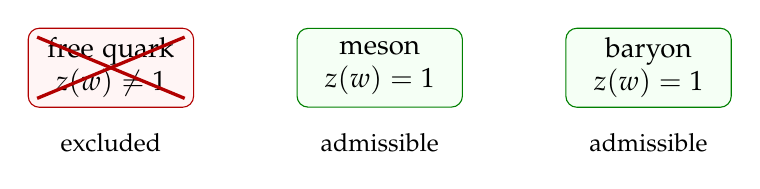
\begin{tikzpicture}[>=Latex, node distance=1.1cm and 1.3cm]
\node[draw=red!70!black, fill=red!4, rounded corners, minimum width=2.1cm, minimum height=1.0cm, align=center] (q) {free quark\\$z(w)\neq 1$};
\node[draw=green!50!black, fill=green!4, rounded corners, minimum width=2.1cm, minimum height=1.0cm, align=center, right=of q] (m) {meson\\$z(w)=1$};
\node[draw=green!50!black, fill=green!4, rounded corners, minimum width=2.1cm, minimum height=1.0cm, align=center, right=of m] (b) {baryon\\$z(w)=1$};
\draw[red!70!black, very thick] ($(q.north west)+(0.12,-0.12)$) -- ($(q.south east)+(-0.12,0.12)$);
\draw[red!70!black, very thick] ($(q.south west)+(0.12,0.12)$) -- ($(q.north east)+(-0.12,-0.12)$);
\node[below=0.2cm of q] {\small excluded};
\node[below=0.2cm of m] {\small admissible};
\node[below=0.2cm of b] {\small admissible};
\end{tikzpicture}
\caption{Confinement as admissible word selection.}
\label{fig:admissible-words}
\end{figure}

The transport-sector string tension is written as
\[
\sigma=\cthree^2\chi_{\QCD}^2,
\]
so the relative Wilson loop obeys
\[
\langle W(C)\rangle_{\mathrm{rel}}\sim e^{-\sigma A(C)}.
\]
The sector-dependent scale $\chi_{\QCD}$ is the minimal notation needed to avoid confusing the hadronic transport channel with the gravitational $\chigeozero$ background; the two channels are linked by the common underlying primitive response $\chiseed$ but not by a naive equality of scales.

\subsection{Transport-side ingredients for the strong-CP theorem}

Define
\begin{equation}
\label{eq:strong-cp}
\bar\theta=\theta_{\mathrm{sheet}}+\arg\det M_u+\arg\det M_d.
\end{equation}
\begin{definition}[Sheet-CP symmetry on the admissible branch]
\label{def:sheet-cp-symmetry}
Define the admissible sheet-CP operator by
\[
\mathcal C_\Sigma:=CP\circ\inv.
\]
\end{definition}

\begin{theorem}[Sheet-CP symmetry protection of strong CP]
\label{thm:sheet-cp-protection}
On the retained admissible branch, the relative action and topological charge satisfy
\[
\mathcal C_\Sigma\,S_{\mathrm{rel}}\,\mathcal C_\Sigma^{-1}=S_{\mathrm{rel}},
\qquad
\mathcal C_\Sigma\,Q\,\mathcal C_\Sigma^{-1}=-Q.
\]
Moreover, by \Cref{prop:gap-lift-full-operator} the regularized transport kernel induces a positive radial operator $H_f>0$ on the admissible sector, and the physical mass map admits the polar form
\[
M_f=U_{f,L}H_fU_{f,R}^\dagger,
\qquad
U_{f,L},U_{f,R}\in SU(3)_F.
\]
Hence
\[
\theta_{\mathrm{sheet}}=0,
\qquad
\arg\det M_f=0,
\]
while weak CP may still survive through
\[
V_{\mathrm{CKM}}=U_{u,L}^\dagger U_{d,L}.
\]
\end{theorem}

\begin{proof}[Proof sketch]
The involution $\inv$ implements the sheet exchange on the admissible branch, so composing it with $CP$ yields an exact symmetry of the relative action while flipping the sign of the topological charge. This forbids a bare $\theta$ deformation on the retained branch. The positive radial transport kernel removes intrinsic determinant phases, and the special-unitary holonomy factors preserve that vanishing while still allowing a nontrivial Jarlskog invariant in the relative family transport.
\end{proof}

\begin{corollary}[Symmetry-protected stability of $\bar\theta=0$ under admissible RG maps]
\label{cor:strong-cp-rg-stability}
In every renormalization scheme that respects $\mathcal C_\Sigma$, $\Padm$, and the carrier structure, the vanishing of
\[
\bar\theta=\theta_{\mathrm{sheet}}+\arg\det M_u+\arg\det M_d
\]
is preserved under the declared RG and matching map.
\end{corollary}

The positive-branch clause is still essential here: the closure statement is about the physical mass map once the admissible transport branch has been fixed, not about an arbitrary unitary dressing of the same singular values. What changes in the present rewrite is the logical source of the null result: the branch no longer relies on a promise not to insert a bad counterterm by hand, but on the symmetry protection encoded by $\mathcal C_\Sigma$ together with the positive-kernel polar decomposition.

\begin{remark}[Admissibility as a unified three-sector motif]
The admissibility pair $(\mathsf{Adm},\Padm)$ acts as a single structural principle with three sector projections:
\begin{itemize}[leftmargin=1.5em, topsep=3pt, itemsep=2pt]
    \item \textbf{Electroweak:} seam-even selection picks the unique light Higgs doublet ($\inv\Phi=+\Phi$).
    \item \textbf{QCD:} center neutrality selects confined hadronic words ($z(w)=1$, $\varepsilon(w)=+1$).
    \item \textbf{Strong CP:} sheet-CP symmetry kills $\theta_{\mathrm{sheet}}$ in the relative action.
\end{itemize}
These are not three independent rules bolted onto different sectors. They are three projections of the same admissible-versus-inadmissible boundary: seam parity, center charge, and sheet exchange are all encoded in the double-cover and involution data of the primitive core. This unification is the conceptual backbone of the transport program.
\end{remark}

\section{Closure theorems from the admissibility complex}
\label{sec:closure-theorems}

The preceding two sections introduced the carrier-compatible geometric and transport architecture. We now state the closure layer in the precise mode used throughout this manuscript: the theorems below are closed statements relative to the admissibility complex, the topological family theorem, and the explicit APS / positivity / reflection-stability inputs collected first.

\begin{definition}[Canonical admissibility complex]
\label{def:admissibility-complex}
Let the admissible Hilbert space factorize as
\[
\mathcal H=\mathcal H_{\Seam}\otimes\mathcal H_c\otimes\mathcal H_\Theta\otimes\mathcal H_t,
\qquad
\mathcal H_{\mathrm{ext}}
:=
\mathcal H\otimes\Lambda(\eta_\Sigma,\eta_c,\eta_\Theta,\eta_g),
\]
with reference normalization
\[
Z_{\mathrm{ref}}[0,0,0]>0,
\]
and symmetry generators
\[
\inv^2=\mathbf 1,
\qquad
Q_\Theta^2=\mathbf 1,
\qquad
Q_\Theta^\dagger=Q_\Theta.
\]
Define the structural selector
\[
P_{\mathrm{str}}:=P_{\Seam,+}P_{\mathrm{sing}}P_\Theta,
\qquad
P_{\Seam,+}:=\frac{\mathbf 1+\inv}{2},
\qquad
P_\Theta:=\frac12(\mathbf 1+Q_\Theta),
\]
with
\[
P_{\mathrm{sing}}:=\frac13(\mathbf 1+Z_c+Z_c^2).
\]
Define the elementary admissibility penalties
\[
K_\Sigma:=\sqrt{\lambda_\Sigma}\,\frac{\mathbf 1-\inv}{2},
\qquad
K_c:=\sqrt{\lambda_c}\,\bigl(\mathbf 1-P_{\mathrm{sing}}\bigr),
\]
\[
K_\Theta:=\sqrt{\lambda_\Theta}\,\frac{\mathbf 1-Q_\Theta}{2},
\qquad
K_g:=\sqrt{\lambda_{\mathrm{gap}}}\,\mathbf 1_{[0,\epsilon_f^2/4)}\!\bigl(P_{\mathrm{str}}D_f^\dagger D_f P_{\mathrm{str}}\bigr),
\]
where the gap penalty is applied only after the structural selector has been fixed.
The first three penalties $K_\Sigma,K_c,K_\Theta$ are Borel functions of mutually commuting
symmetry generators and commute canonically. For $K_g$ the commutation with the structural
penalties holds provided
\[
[D_f^\dagger D_f,\inv]=[D_f^\dagger D_f,P_{\mathrm{sing}}]=[D_f^\dagger D_f,Q_\Theta]=0
\qquad
\text{on }\mathrm{Ran}(P_{\mathrm{str}}),
\]
which is assumed on the admissible transport branch. The admissibility differential is
\[
Q_{\mathrm{adm}}
:=
\eta_\Sigma^\dagger K_\Sigma
+\eta_c^\dagger K_c
+\eta_\Theta^\dagger K_\Theta
+\eta_g^\dagger K_g,
\]
and the admissibility Laplacian is
\[
\Delta_{\mathrm{adm}}:=\{Q_{\mathrm{adm}},Q_{\mathrm{adm}}^\dagger\}.
\]
\end{definition}

\begin{lemma}[Canonical nilpotency and Hodge projector]
\label{lem:admissibility-nilpotency}
\label{lem:hodge-admissibility-projector}
On the admissible reduced datum,
\[
Q_{\mathrm{adm}}^2=0,
\qquad
\Delta_{\mathrm{adm}}
=
K_\Sigma^2+K_c^2+K_\Theta^2+K_g^2
=
\Kadm,
\]
with
\[
\Kadm
:=
\lambda_\Sigma\frac{\mathbf 1-\inv}{2}
+\lambda_c\bigl(\mathbf 1-P_{\mathrm{sing}}\bigr)
+\lambda_\Theta\frac{\mathbf 1-Q_\Theta}{2}
+\lambda_{\mathrm{gap}}\,\mathbf 1_{[0,\epsilon_f^2/4)}\!\bigl(P_{\mathrm{str}}D_f^\dagger D_f P_{\mathrm{str}}\bigr),
\]
and
\[
\Padm
:=
\Pi_{\ker\Delta_{\mathrm{adm}}}
=
\operatorname*{s-lim}_{\beta\to\infty}e^{-\beta\Kadm}.
\]
Thus $\Padm$ is the Hodge projector onto the harmonic admissible sector rather than a
separately declared filter.
\end{lemma}

\begin{proof}[Proof sketch]
The auxiliary generators $\eta_i^\dagger$ anticommute, so the square of $Q_{\mathrm{adm}}$
is controlled by the commutators of the corresponding $K_i$. Canonical commutation kills the
mixed terms, leaving $Q_{\mathrm{adm}}^2=0$ and $\Delta_{\mathrm{adm}}=\Kadm$. The
zero-temperature limit therefore projects exactly onto the harmonic admissible sector.
\end{proof}

\begin{corollary}[Factorized selector on the admissible branch]
\label{cor:factorized-admissibility-selector}
If one further writes
\[
P_{\mathrm{gap}}:=\mathbf 1_{[\epsilon_f^2/4,\infty)}\!\bigl(P_{\mathrm{str}}D_f^\dagger D_f P_{\mathrm{str}}\bigr),
\]
then
\[
\Padm=P_{\mathrm{str}}P_{\mathrm{gap}},
\qquad
P_{\mathrm{str}}:=P_{\Seam,+}P_{\mathrm{sing}}P_\Theta.
\]
So the familiar factorized selector is retained only as a corollary of the canonical
admissibility complex.
\end{corollary}

\begin{theorem}[Master closure from canonical doubling]
\label{thm:master-closure}
\label{ass:remaining-closure-inputs}
Let $\Tmin^{\mathrm{adm}}$ be admissible and let $X_b$ be the canonical double across $\Seam$.
Write
\[
D_b=
\begin{pmatrix}
0&D_{\mathrm{rel}}^-\\
D_{\mathrm{rel}}^+&0
\end{pmatrix},
\qquad
Q_{\mathrm{tot}}:=Q_{\mathrm{adm}}+d_\Sigma+d_\Sigma^\dagger,
\qquad
\Delta_{\mathrm{tot}}:=\{Q_{\mathrm{tot}},Q_{\mathrm{tot}}^\dagger\}.
\]
Then all of the following are derived on the same datum:
\begin{enumerate}[label=(\arabic*), leftmargin=1.5em, topsep=3pt, itemsep=2pt]
    \item the Calder\'on projector of $D_b$ induces $\APSdom$ canonically;
    \item the family pairing data are induced canonically, so no separate $\APSfam$ datum remains;
    \item
    \[
    \Padm:=\Pi_{\ker \Delta_{\mathrm{adm}}},
    \]
    and the doubled total closure package preserves $\mathrm{Ran}(\Padm)$;
    \item
    \[
    \chi_{\mathrm{orb}}(X_f)=-2,
    \qquad
    F\simeq H^1(X_f,\mathbb C)\simeq \mathbb C^3,
    \qquad
    N_{\mathrm{fam}}=3;
    \]
    \item the harmonic determinant line is parallel and therefore
    \[
    \mathrm{Hol}(\nabla_F)\subset SU(3)_F;
    \]
    \item admissible bosonic and fermionic reflection positivity hold on $\mathrm{Ran}(\Padm)$;
    \item $\Padm\Hrel\Padm$ is lower bounded and coercive.
\end{enumerate}
\end{theorem}

\begin{definition}[Relative generating functional]
\label{def:relative-generating-functional}
The relative Euclidean generating functional is normalized as
\[
Z_{\mathrm{rel}}[J,\eta,\bar\eta]
:=
\frac{Z_{\mathrm{adm}}[J,\eta,\bar\eta]}{Z_{\mathrm{ref}}[0,0,0]}.
\]
The reference sector is therefore a fixed normalizing denominator rather than a second fluctuating measure that would mix with admissible positivity.
\end{definition}

\begin{lemma}[Admissible reflection positivity]
\label{lem:admissible-reflection-positivity}
Assume
\[
[\Theta,P_\Theta]=0,
\qquad
\Theta\Padm=\Padm\Theta,
\]
the admissible bosonic kernel satisfies the primitive positivity theorem
\Cref{ass:bernstein-positivity} and is reflection-stable on the admissible sector, and the
admissible fermionic CAR kernel is reflection positive on that same sector. Then every
admissible observable $O$ supported in $\tau>0$ satisfies
\[
\langle \Theta O,O\rangle_{\mathrm{rel}}
=
\frac{1}{Z_{\mathrm{ref}}[0,0,0]}
\langle \Theta O,O\rangle_{\mathrm{adm}}
\ge 0.
\]
\end{lemma}

\begin{proof}[Proof sketch]
The quotient form \Cref{def:relative-generating-functional} removes the reference sector from the positivity problem and leaves only a constant denominator. The bosonic sector then follows from the Bernstein superposition of positive heat kernels together with reflection stability on admissible observables. The fermionic sector is handled in the CAR version of reflection positivity, equivalently through positivity of the reflected quadratic kernel or the corresponding Pfaffian form on the admissible subspace.
\end{proof}

\begin{theorem}[Operative admissibility selector]
Under \Cref{def:admissibility-complex,lem:admissibility-nilpotency,lem:hodge-admissibility-projector,ass:remaining-closure-inputs}, the operator $\Padm$ is idempotent on the retained branch and realizes the admissibility predicate on all sectors used by the closed compiler statements:
\[
\mathsf{Adm}(X)=1
\quad\Longleftrightarrow\quad
\Padm X = X.
\]
\end{theorem}

\begin{proof}[Proof sketch]
By \Cref{lem:hodge-admissibility-projector}, $\Padm$ is the orthogonal projector onto the
harmonic admissible sector of the complex and therefore idempotent by construction. On the
admissible branch, \Cref{cor:factorized-admissibility-selector} recovers the older product form
as a corollary. The predicate and operator languages agree once the positive transport sector is
fixed.
\end{proof}

\begin{theorem}[Topological family closure on the admissible branch]
By \Cref{thm:master-closure,thm:orbifold-aps-family-master,cor:boundary-bulk-occupancy},
\[
\chi_{\mathrm{orb}}(X_f)=-2,
\qquad
F\cong\mathbb C^3,
\qquad
N_{\mathrm{fam}}=3.
\]
Consequently
\[
\Oadm=N_{\mathrm{fam}}\dim S^+=3\times 16=48,
\qquad
\deltatop=\Oadm\,\cthree^4.
\]
\end{theorem}

\begin{proof}[Proof sketch]
This theorem is now a direct consequence of the master closure theorem from Section~6. The
topological family closure and the orbifold corner count have already been compressed there
into one statement, so the present layer merely records the corresponding admissibility
consequence.
\end{proof}

\begin{theorem}[Bosonic index and local spectral-scale closure]
On the admissible branch,
\[
\Ind_{\mathrm{rel}}^{\Padm}(\mathcal B_{E_2}^+)=1,
\qquad
\Ind_{\mathrm{rel}}^{\Padm}(\mathcal B_{E_3}^+)=0,
\]
so the unique light seam-even bosonic zero mode is
\[
\Phi\in\Gamma(E_2)\cong(1,2)_{1/2},
\qquad
\inv\Phi=+\Phi.
\]
Moreover the same closure layer yields
\[
\Mpl^2=\frac{\chigeozero^2}{2\pi^2},
\qquad
G_N\chigeozero^2=\frac{\pi}{4},
\qquad
\vgeo^2=Z_H\,\frac{\mu_\Phi^2(\chigeozero)}{\lambda_\Phi},
\qquad
\vgeo=\Mpl\,\gcar\,\beta_{\mathrm{rad}}^2
\exp\!\left[-\frac{\alpha^{-1}(0)+\delta_{\mathrm{ph}}}{5}\right].
\]
\end{theorem}

\begin{proof}[Proof sketch]
The bosonic sector is treated as a genuine Callias / Dirac / Dolbeault-type index problem rather than a scalar counting exercise. Relative heat-kernel closure together with \Cref{prop:canonical-bosonic-normalization,lem:two-sheet-zero-mode-normalization} produces the Einstein branch, the canonical Higgs normalization, and the seam-even zero-mode formula for $\vgeo$, with the Newton relation as a corollary of the reduced-Planck normalization.
\end{proof}

\begin{theorem}[Holonomy form of the Yukawa matrices]
On the admissible branch, each fermion sector admits the factorization
\[
Y_f=D_{L,f}U_fD_{R,f},
\qquad
U_f\in SU(3)_F,
\]
and, in the family basis,
\[
(Y_f)_{ij}
=
\lambdaY^{L^L_{f,i}+L^R_{f,j}}
\left\langle e_i,\mathrm{Hol}_{\Gamma_{ij}}(\nabla_F)e_j\right\rangle.
\]
The diagonal path-length rows \Cref{eq:path-length-yukawa} are the singular-value reduction of this matrix statement.
\end{theorem}

\begin{proof}[Proof sketch]
The finite $C_6$ transport geometry fixes the graph-distance weights, while the residual bounded holonomy factors are absorbed into $SU(3)_F$ transport matrices. The diagonal ladder formulas arise once left and right admissible words are paired on the same singular-value channel.
\end{proof}

\begin{definition}[Center-neutral admissible algebra]
Let
\[
\Asing
:=
\overline{\mathrm{span}}\{A_w:\ z(w)=1,\ \varepsilon(w)=+1,\ \Padm A_w=A_w\}.
\]
\end{definition}

\begin{theorem}[Hadronic space and confinement closure]
On the admissible branch, the physical hadronic Hilbert space is
\[
\Hhad:=\overline{\Asing|\Omega\rangle}.
\]
All physical hadronic states lie in $\Hhad$, while color-nonsinglet free-word sectors are removed by $\Padm$.
\end{theorem}

\begin{proof}[Proof sketch]
Center neutrality and seam-evenness are already the carrier-side admissibility rules for physical hadrons. Passing to the norm closure of the singlet admissible algebra acting on the vacuum gives the completed hadronic space, and no state with $z(w)\neq 1$ survives the selector.
\end{proof}

\begin{theorem}[Anomaly cancellation and seam inflow]
On the admissible branch,
\[
I_6^{\mathrm{tot}}=0,
\qquad
\delta_\Lambda S_{\mathrm{bulk}}+\delta_\Lambda S_{\eta,\Seam}=0.
\]
\end{theorem}

\begin{proof}[Proof sketch]
The one-family packet $S^+$ is exactly the anomaly-free Standard Model family including $\nu^c$. The remaining seam contribution is carried by the relative $\eta$ term, so gauge variation cancels between bulk and seam sectors rather than being left as an uncancelled boundary defect.
\end{proof}

\begin{theorem}[Strong-CP closure on the admissible branch]
\label{thm:strong-cp-closure}
Define
\[
Z_{\mathrm{adm}}(\bar\theta)
:=
\int e^{-S_{\mathrm{adm}}}e^{i\bar\theta Q}\,d\mu_{\mathrm{adm}},
\qquad
Q=\frac{1}{32\pi^2}\int \tr(G\wedge G).
\]
On the admissible branch,
\[
\theta_{\mathrm{sheet}}=0,
\qquad
\arg\det M_u=\arg\det M_d=0,
\qquad
\bar\theta=0.
\]
Moreover,
\[
\bigl|Z_{\mathrm{adm}}(\bar\theta)\bigr|\le Z_{\mathrm{adm}}(0),
\]
so the free energy
\[
F(\bar\theta):=-V^{-1}\log Z_{\mathrm{adm}}(\bar\theta)
\]
satisfies $F(\bar\theta)\ge F(0)$. If the CP-even admissible vacuum is unique, its minimum lies at $\bar\theta=0$. At the same time weak CP may survive through
\[
V_{\mathrm{CKM}}=U_{u,L}^\dagger U_{d,L}.
\]
\end{theorem}

\begin{proof}[Proof sketch]
\Cref{thm:sheet-cp-protection,cor:strong-cp-rg-stability} supply the symmetry-protected vanishing of $\theta_{\mathrm{sheet}}$ and of the determinant phases on the retained branch. Positivity of the admissible measure then implies the standard free-energy inequality, so the CP-even branch minimizes at $\bar\theta=0$ once the admissible vacuum is unique. Weak CP may still survive through the relative family holonomies encoded in $V_{\mathrm{CKM}}$.
\end{proof}

\begin{theorem}[Reflection positivity on the admissible sector]
\label{thm:reflection-positivity-admissible}
Under the admissibility complex and the setup of \Cref{def:relative-generating-functional,lem:admissible-reflection-positivity}, every admissible observable $O$ with support in $\tau>0$ satisfies
\[
\langle \Theta O,O\rangle_{\mathrm{rel}}\ge 0.
\]
\end{theorem}

\begin{proof}[Proof sketch]
Invoke \Cref{lem:admissible-reflection-positivity}. The point of the quotient normalization is that the reference sector contributes only the constant denominator $Z_{\mathrm{ref}}[0,0,0]$ and therefore does not spoil positivity on admissible observables.
\end{proof}

\begin{theorem}[Lorentzian reconstruction on \texorpdfstring{$\Padm$}{Padm}]
\label{thm:lorentzian-reconstruction}
Under the same hypotheses, the admissible Euclidean theory reconstructs a self-adjoint Lorentzian Hamiltonian on the $\Padm$ sector.
\end{theorem}

\begin{proof}[Proof sketch]
With \Cref{thm:reflection-positivity-admissible} in hand, the bosonic part follows the usual Osterwalder--Schrader reconstruction, while the fermionic part follows the corresponding CAR reconstruction on the admissible sector. The commuting relations between $\Theta$, $P_\Theta$, and $\Padm$ ensure that the reconstructed Hilbert space remains inside the retained admissible branch.
\end{proof}

\begin{theorem}[Admissible vacuum existence at finite volume or with declared cutoff]
\label{thm:admissible-vacuum-existence}
Assume finite volume or a declared cutoff, weak-* compactness of $\Vadm$, and
lower boundedness plus coercivity of $\Padm\Hrel\Padm$. Then the admissible
vacuum exists as
\[
\rho^\ast=\argmin_{\rho\in\Vadm}\tr(\rho\Hrel),
\]
and its renormalized seam vacuum energy is denoted by $\Lambda_{\Seam,\mathrm{ren}}$.
\end{theorem}

\begin{proof}
The direct method applies on $\Vadm$ under the stated compactness and coercivity
assumptions. The renormalized seam residue supplies the vacuum-energy
identification in the same declared scheme.
\end{proof}

\begin{theorem}[Nonperturbative admissible QFT closure]
\label{thm:nonperturbative-admissible-qft}
Let
\[
m_*:=\min\left\{\frac{\epsilon_f}{2},\,m_-,\,m_3\right\}.
\]
Assume the transport gap estimate of \Cref{prop:gap-lift-full-operator} together with the positivity bounds of \Cref{thm:callias-higgs-selection}. Then, after removing the exact gauge zero modes, the reconstructed admissible Hamiltonian satisfies
\[
\operatorname{spec}(H_{\mathrm{adm}})\cap(0,m_*)=\varnothing.
\]
Hence connected admissible Euclidean correlators obey exponential clustering:
\[
\bigl|\langle O_1(x)O_2(0)\rangle_c\bigr|
\le
C_{12}e^{-m_*|x|}.
\]
\end{theorem}

\begin{proof}[Proof sketch]
The transport gap and the bosonic positivity bounds give a strict positive lower bound on all admissible excitations above the exact gauge zero modes. Reflection positivity and Lorentzian reconstruction convert the Euclidean gap into a Lorentzian spectral gap. Exponential clustering follows from that gap on the admissible sector.
\end{proof}

\begin{definition}[Stable record algebra from the admissible gap]
\label{def:stable-record-algebra}
Let
\[
\tau_*:=\frac{1}{m_*}.
\]
For a tolerance $\varepsilon>0$, define
\[
\Arec(t)
:=
\left\{
O\in\mathfrak A_{\mathrm{adm}}
:\ \|[O(t),O(t')]\|\le\varepsilon
\text{ for } |t-t'|>\tau_*
\right\}.
\]
\end{definition}

\begin{proposition}[Stable records from gap and clustering]
Under \Cref{thm:nonperturbative-admissible-qft}, the algebra $\Arec(t)$ defines the slow, robust sector singled out by the admissible mass gap. Record observables are therefore a dynamical consequence of gap plus clustering rather than an independent philosophical postulate.
\end{proposition}

\begin{proof}[Proof sketch]
The spectral gap suppresses long-time commutators by the same exponential scale that controls connected correlators. Therefore operators whose support is carried by the low-frequency admissible sector become approximately commuting on time separations larger than $\tau_*=1/m_*$, which is exactly the stability criterion built into \Cref{def:stable-record-algebra}.
\end{proof}

\begin{definition}[Observer algebra and prediction semantics]
\label{def:observer-algebra-prediction}
Choose $\Aobs\subset\Arec$ to be a maximal stable abelian subalgebra. For any operational query $Q$ represented by a spectral projector $E_Q(\Delta)$, define
\[
\Pred(Q):=\tr(\rho_tE_Q(\Delta)).
\]
This is the main-text prediction semantics used on the admissible branch; appendix-level bookkeeping only decorates it with extra experimental metadata.
\end{definition}

\begin{remark}[Horizons as modular inner seams]
The same seam grammar extends to horizon physics by treating horizons as modular inner seams. In that reading one works with algebraic splits or code-subspace factorizations adapted to the horizon sector, rather than declaring an exact tensor-product factorization as primitive structure.
\end{remark}

\section{Particle and mass compiler}

This section is the phenomenological heart of the manuscript. It is not meant to flatten all
rows into one uniform notion of prediction. Instead it makes the relation between derived theorem
outputs and intrinsic observation rows explicit: a declared numerical preconditioner, a
kernel-output map, and a mass ledger that separates internal theorem outputs from their
observation-surface images.
Accordingly this section is best read through three ledgers:
\begin{itemize}[leftmargin=1.5em, topsep=3pt, itemsep=2pt]
    \item a \emph{primary intrinsic-observation ledger} for the narrow main-text comparison surface in \Cref{tab:benchmark},
    \item \emph{mass-closure ledgers} for fermion, electroweak, and hadronic rows in \Cref{tab:sm-mass-ledger-ew,tab:sm-mass-ledger-quarks},
    \item and a \emph{supplementary appendix ledger} for exploratory or optional rows that are kept outside the closed theorem surface.
\end{itemize}

\begin{definition}[Intrinsic and observation surfaces]
\label{def:intrinsic-observation-surfaces}
We write $\mathcal S_{\mathrm{int}}$ for the intrinsic closure surface generated before
comparison, containing in particular the internal compiler masses $\hat m_f$, the transport
outputs, and the derived geometric parameters. The observation surface is
\[
\mathcal S_{\mathrm{obs}}:=\mathcal R_{\mathrm{TOE}}(\mathcal S_{\mathrm{int}}),
\]
that is, the scheme-specified comparison image after matching, thresholds, and observable
conventions are imposed. In practical finite-threshold computations one approximates this surface
through the numerical preconditioner $\mathcal R_{\SM}$. The first surface is theorem-facing; the
second is the observation-facing interface used by the ledgers below.
\end{definition}

\begin{figure}[p]
\centering
\scriptsize
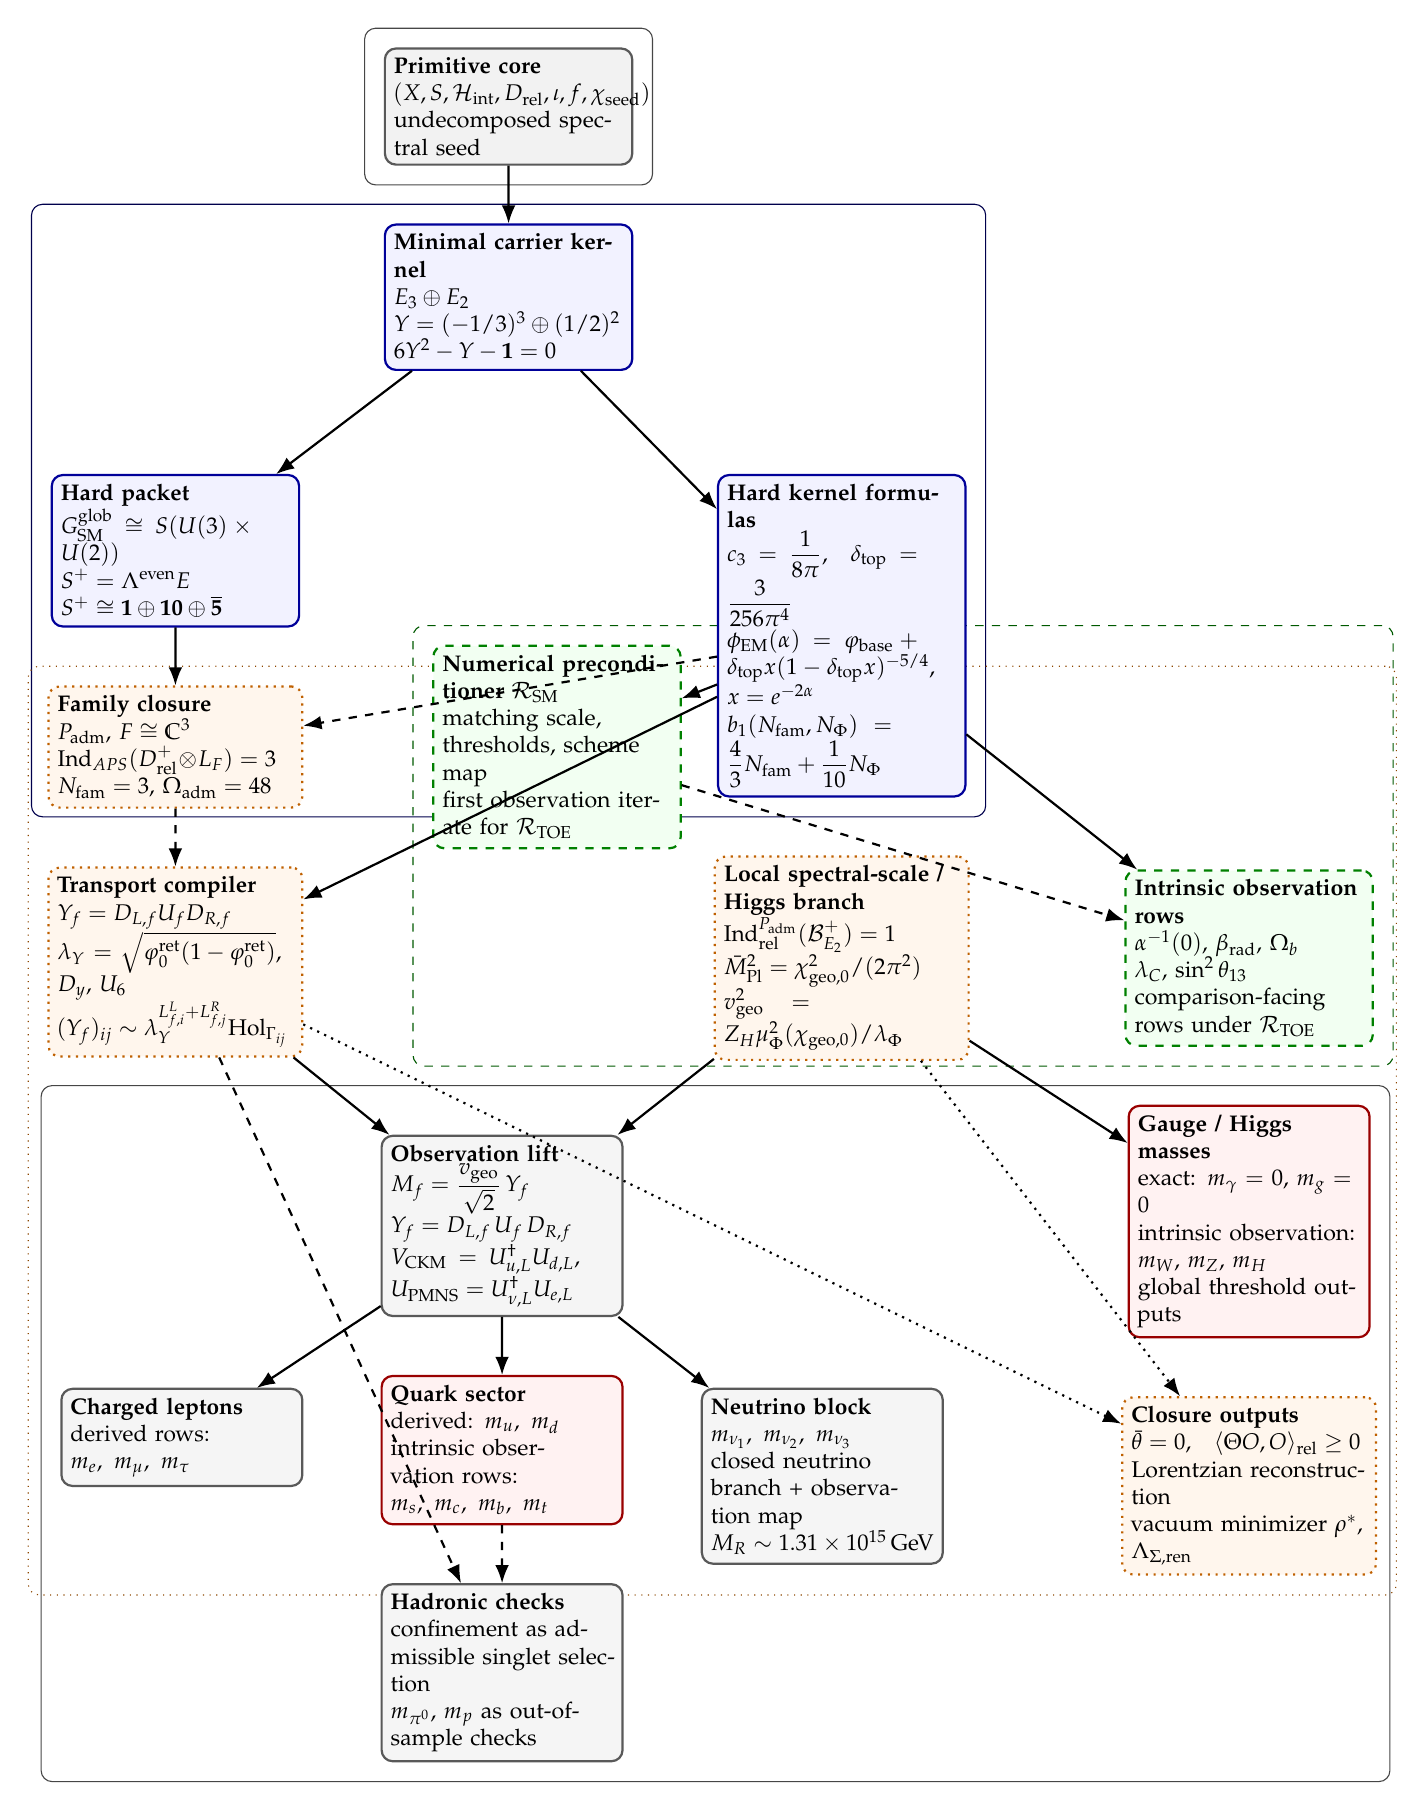
\begin{tikzpicture}[
    scale=0.82,
    transform shape,
    >=Latex,
    node distance=9mm and 11mm,
    primitive/.style={
        draw=gray!70!black,
        thick,
        rounded corners,
        fill=gray!10,
        align=left,
        text width=3.55cm,
        inner sep=4pt
    },
    hard/.style={
        draw=blue!60!black,
        thick,
        rounded corners,
        fill=blue!5,
        align=left,
        text width=3.55cm,
        inner sep=4pt
    },
    bridge/.style={
        draw=green!50!black,
        dashed,
        thick,
        rounded corners,
        fill=green!5,
        align=left,
        text width=3.55cm,
        inner sep=4pt
    },
    closure/.style={
        draw=orange!75!black,
        dotted,
        thick,
        rounded corners,
        fill=orange!7,
        align=left,
        text width=3.65cm,
        inner sep=4pt
    },
    output/.style={
        draw=gray!70!black,
        thick,
        rounded corners,
        fill=gray!8,
        align=left,
        text width=3.45cm,
        inner sep=4pt
    },
    anchorrow/.style={
        draw=red!60!black,
        thick,
        rounded corners,
        fill=red!5,
        align=left,
        text width=3.45cm,
        inner sep=4pt
    },
    flow/.style={->, thick},
    aux/.style={->, thick, dashed},
    cond/.style={->, thick, dotted}
]

\node[primitive] (core) {%
\textbf{Primitive core}\\
$(X,S,\Hint,D_{\mathrm{rel}},\iota,f,\chiseed)$\\
undecomposed spectral seed
};

\node[hard, below=of core] (carrier) {%
\textbf{Minimal carrier kernel}\\
$E_3 \oplus E_2$\\
$Y=(-1/3)^3\oplus(1/2)^2$\\
$6Y^2-Y-\mathbf 1=0$
};

\node[hard, below left=16mm and 13mm of carrier] (familypacket) {%
\textbf{Hard packet}\\
$G_{\mathrm{SM}}^{\mathrm{glob}} \cong S(U(3)\times U(2))$\\
$S^+=\Lambda^{\mathrm{even}}E$\\
$S^+ \cong \mathbf 1 \oplus \mathbf{10} \oplus \overline{\mathbf 5}$
};

\node[hard, below right=16mm and 13mm of carrier] (seed) {%
\textbf{Hard kernel formulas}\\
$c_3=\dfrac{1}{8\pi}$,\quad
$\delta_{\mathrm{top}}=\dfrac{3}{256\pi^4}$\\
$\phi_{\mathrm{EM}}(\alpha)=\phibase+\deltatop x(1-\deltatop x)^{-5/4}$,\ $x=e^{-2\alpha}$\\
$b_1(N_{\mathrm{fam}},N_\Phi)=\dfrac43N_{\mathrm{fam}}+\dfrac1{10}N_\Phi$
};

\node[closure, below=of familypacket] (familybridge) {%
\textbf{Family closure}\\
$\Padm$, $F\cong\mathbb C^3$\\
$\mathrm{Ind}_{APS}(D^+_{\mathrm{rel}}\!\otimes\!L_F)=3$\\
$N_{\mathrm{fam}}=3$, $\Omega_{\mathrm{adm}}=48$
};

\node[closure, below=of seed] (chi) {%
\textbf{Local spectral-scale / Higgs branch}\\
$\mathrm{Ind}^{\Padm}_{\mathrm{rel}}(\mathcal B^+_{E_2})=1$\\
$\bar M_{\mathrm{Pl}}^2=\chigeozero^2/(2\pi^2)$\\
$\vgeo^2=Z_H\mu_\Phi^2(\chigeozero)/\lambda_\Phi$
};

\node[bridge, right=20mm of familybridge] (comparison) {%
\textbf{Numerical preconditioner $\mathcal R_{\mathrm{SM}}$}\\
matching scale, thresholds, scheme map\\
first observation iterate for $\mathcal R_{\mathrm{TOE}}$
};

\node[closure, below=of familybridge] (transport) {%
\textbf{Transport compiler}\\
$Y_f=D_{L,f}U_fD_{R,f}$\\
$\lambda_Y=\sqrt{\phiz(1-\phiz)}$, $D_y$, $U_6$\\
$(Y_f)_{ij}\sim \lambda_Y^{L^L_{f,i}+L^R_{f,j}}\mathrm{Hol}_{\Gamma_{ij}}$
};

\node[output, below right=12mm and 12mm of transport] (massmatrix) {%
\textbf{Observation lift}\\
$M_f=\dfrac{\vgeo}{\sqrt 2}\,Y_f$\\
$Y_f=D_{L,f}\,U_f\,D_{R,f}$\\
$V_{\mathrm{CKM}}=U_{u,L}^\dagger U_{d,L}$,\quad
$U_{\mathrm{PMNS}}=U_{\nu,L}^\dagger U_{e,L}$
};

\node[bridge, right=24mm of chi] (benchmarks) {%
\textbf{Intrinsic observation rows}\\
$\alpha^{-1}(0)$,\ $\beta_{\mathrm{rad}}$,\ $\Omega_b$\\
$\lambda_C$,\ $\sin^2\theta_{13}$\\
comparison-facing rows under $\mathcal R_{\mathrm{TOE}}$
};

\node[anchorrow, below=of benchmarks] (bosons) {%
\textbf{Gauge / Higgs masses}\\
exact: $m_\gamma=0$, $m_g=0$\\
intrinsic observation: $m_W$, $m_Z$, $m_H$\\
global threshold outputs
};

\node[output, below left=11mm and 12mm of massmatrix] (leptons) {%
\textbf{Charged leptons}\\
derived rows:\\
$m_e,\ m_\mu,\ m_\tau$
};

\node[anchorrow, below=of massmatrix] (quarks) {%
\textbf{Quark sector}\\
derived: $m_u,\ m_d$\\
intrinsic observation rows: $m_s,\ m_c,\ m_b,\ m_t$
};

\node[output, below right=11mm and 12mm of massmatrix] (neutrinos) {%
\textbf{Neutrino block}\\
$m_{\nu_1},\ m_{\nu_2},\ m_{\nu_3}$\\
closed neutrino branch + observation map\\
$M_R \sim 1.31\times 10^{15}\,\mathrm{GeV}$
};

\node[output, below=of quarks] (hadrons) {%
\textbf{Hadronic checks}\\
confinement as admissible singlet selection\\
$m_{\pi^0}$,\ $m_p$ as out-of-sample checks
};

\node[closure, below=of bosons] (cp) {%
\textbf{Closure outputs}\\
$\bar\theta=0$,\quad $\langle\Theta O,O\rangle_{\mathrm{rel}}\ge 0$\\
Lorentzian reconstruction\\
vacuum minimizer $\rho^\ast$, $\Lambda_{\Seam,\mathrm{ren}}$
};

\draw[flow] (core) -- (carrier);
\draw[flow] (carrier) -- (familypacket);
\draw[flow] (carrier) -- (seed);
\draw[flow] (familypacket) -- (familybridge);
\draw[aux] (seed) -- (familybridge);
\draw[flow] (seed) -- (comparison);
\draw[flow] (seed) -- (benchmarks);
\draw[flow] (seed) -- (transport);
\draw[aux] (familybridge) -- (transport);
\draw[flow] (chi) -- (bosons);
\draw[flow] (chi) -- (massmatrix);
\draw[flow] (transport) -- (massmatrix);
\draw[aux] (comparison) -- (benchmarks);
\draw[flow] (massmatrix) -- (leptons);
\draw[flow] (massmatrix) -- (quarks);
\draw[flow] (massmatrix) -- (neutrinos);
\draw[aux] (transport) -- (hadrons);
\draw[aux] (quarks) -- (hadrons);
\draw[cond] (transport) -- (cp);
\draw[cond] (chi) -- (cp);

\begin{scope}[on background layer]
    \node[draw=gray!55!black, rounded corners, inner sep=7pt,
          fit=(core)] {};
    \node[draw=blue!30!black, rounded corners, inner sep=7pt,
          fit=(carrier)(familypacket)(seed)] {};
    \node[draw=green!35!black, dashed, rounded corners, inner sep=7pt,
          fit=(comparison)(benchmarks)] {};
    \node[draw=orange!55!black, dotted, rounded corners, inner sep=7pt,
          fit=(familybridge)(chi)(transport)(cp)] {};
    \node[draw=gray!55!black, rounded corners, inner sep=7pt,
          fit=(bosons)(massmatrix)(leptons)(quarks)(neutrinos)(hadrons)] {};
\end{scope}
\end{tikzpicture}
\caption{Carrier-first compiler from reduced datum to explicit particle-content and mass
surfaces. Gray nodes denote the reduced datum, blue nodes are exact algebraic carrier/kernel
statements, orange nodes are conditional closure statements, green nodes denote the matched
intrinsic observation layer and its numerical preconditioner, and gray/red nodes are compact
output surfaces. The figure intentionally separates exact algebraic and conditional theorem
outputs from matched observation rows.}
\label{fig:compiler-to-masses}
\end{figure}

The diagram in \Cref{fig:compiler-to-masses} is epistemically layered: it visualizes one
compiler flow, not one uniform status class. Exact massless gauge directions, conditional
charged-lepton rows, matched heavy-mass observation rows, neutrino observation rows, and
conditional hadronic rows are shown together only to display the architecture, not to erase
their different proof roles.

A second, more compressed projection of that same surface is shown in \Cref{fig:epistemic-output-matrix}. It does not add a new theorem; it makes the manuscript's status discipline readable at the level of output types.

\begin{figure}[t]
\centering
\scriptsize
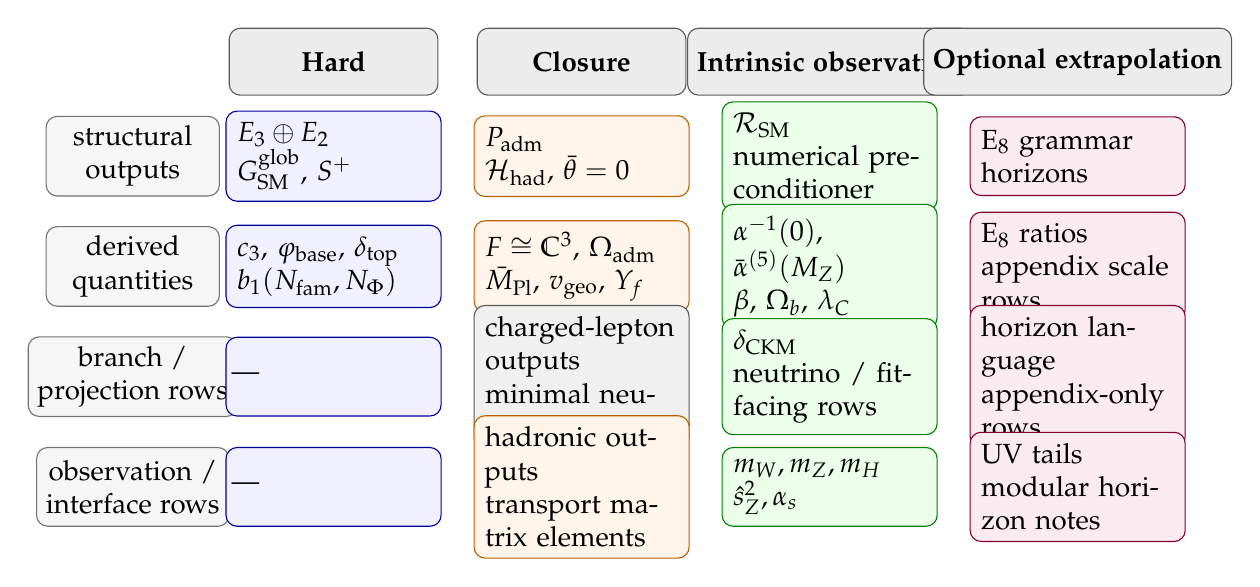
\begin{tikzpicture}[
    hdr/.style={draw=black!65, fill=gray!15, rounded corners, minimum width=2.65cm, minimum height=0.85cm, align=center, font=\bfseries},
    rowhdr/.style={draw=black!55, fill=gray!7, rounded corners, minimum width=2.2cm, minimum height=1.0cm, align=center},
    hard/.style={draw=blue!60!black, fill=blue!6, rounded corners, text width=2.45cm, minimum height=1.0cm, align=left, inner sep=4pt},
    closure/.style={draw=orange!75!black, fill=orange!8, rounded corners, text width=2.45cm, minimum height=1.0cm, align=left, inner sep=4pt},
    bridge/.style={draw=green!50!black, fill=green!8, rounded corners, text width=2.45cm, minimum height=1.0cm, align=left, inner sep=4pt},
    branchrow/.style={draw=gray!70!black, fill=gray!12, rounded corners, text width=2.45cm, minimum height=1.0cm, align=left, inner sep=4pt},
    cond/.style={draw=purple!70!black, fill=purple!8, rounded corners, text width=2.45cm, minimum height=1.0cm, align=left, inner sep=4pt}
]
\node[hdr] at (0,0) {Hard};
\node[hdr] at (3.15,0) {Closure};
\node[hdr] at (6.3,0) {Intrinsic observation};
\node[hdr] at (9.45,0) {Optional extrapolation};

\node[rowhdr] at (-2.55,-1.2) {structural\\outputs};
\node[rowhdr] at (-2.55,-2.6) {derived\\quantities};
\node[rowhdr] at (-2.55,-4.0) {branch /\\projection rows};
\node[rowhdr] at (-2.55,-5.4) {observation /\\interface rows};

\node[hard] at (0,-1.2) {$E_3\oplus E_2$\\$G_{\SM}^{\mathrm{glob}}$, $S^+$};
\node[closure] at (3.15,-1.2) {$\Padm$\\$\Hhad$, $\bar\theta=0$};
\node[bridge] at (6.3,-1.2) {$\mathcal R_{\SM}$\\numerical preconditioner};
\node[cond] at (9.45,-1.2) {E$_8$ grammar\\horizons};

\node[hard] at (0,-2.6) {$\cthree$, $\phibase$, $\deltatop$\\$\bone(N_{\mathrm{fam}},N_\Phi)$};
\node[closure] at (3.15,-2.6) {$F\cong\mathbb C^3$, $\Omega_{\mathrm{adm}}$\\$\Mpl$, $\vgeo$, $Y_f$};
\node[bridge] at (6.3,-2.6) {$\alpha^{-1}(0)$, $\bar\alpha^{(5)}(M_Z)$\\$\beta$, $\Omega_b$, $\lambda_C$};
\node[cond] at (9.45,-2.6) {E$_8$ ratios\\appendix scale rows};

\node[hard] at (0,-4.0) {---};
\node[branchrow] at (3.15,-4.0) {charged-lepton outputs\\minimal neutrino branch};
\node[bridge] at (6.3,-4.0) {$\delta_{\mathrm{CKM}}$\\neutrino / fit-facing rows};
\node[cond] at (9.45,-4.0) {horizon language\\appendix-only rows};

\node[hard] at (0,-5.4) {---};
\node[closure] at (3.15,-5.4) {hadronic outputs\\transport matrix elements};
\node[bridge] at (6.3,-5.4) {$m_W,m_Z,m_H$\\$\hat s_Z^2,\alpha_s$};
\node[cond] at (9.45,-5.4) {UV tails\\modular horizon notes};
\end{tikzpicture}
\caption{Epistemic output matrix. Columns encode the manuscript's truth/status classes; rows encode output mode. The point is to stop exact algebraic outputs, conditional closure rows, matched observation rows, and optional extrapolations from looking like one homogeneous notion of prediction.}
\label{fig:epistemic-output-matrix}
\end{figure}

\subsection{RG map for compiler outputs}
\label{sec:rg-map-compiler-outputs}

The symbol $\mathcal R_{\SM}$ denotes the declared comparison map from TFPT outputs to scheme-specified observables. Here it is the bookkeeping package
\[
\mathcal R_{\SM}
=
\left(
\begin{array}{l}
\mu_{\mathrm{match}}=M_Z,\ \{\mu_{\mathrm{thr}}\}=\{m_c,m_b,m_\tau,m_t\},\\
\text{running convention},\ \text{scheme conversion},\ \text{observable map}
\end{array}
\right),
\]
and we write
\[
\bar\alpha^{(5)}(M_Z):=\alpha_{\mathrm{em}}^{\overline{\mathrm{MS}},\,n_f=5}(M_Z).
\]
with the following restricted interpretation in the main text:
\begin{itemize}[leftmargin=1.5em, topsep=3pt, itemsep=2pt]
    \item $\alpha^{-1}(0)$ is compared in the Thomson-limit on-shell convention, with the CODATA 2022 / NIST value taken as the normative low-energy reference rather than the separate PDG electroweak extraction from $a_e$,
    \item $\bar\alpha^{(5)}(M_Z)^{-1}$ is compared after the declared threshold map with $\{\mu_{\mathrm{thr}}\}=\{m_c,m_b,m_\tau,m_t\}$ into the $\overline{\mathrm{MS}}$ language at $\mu=M_Z$,
    \item neutrino-angle rows use the NuFIT normal-ordering reference snapshot based on data available through November 2025,
    \item the $\Omega_b$ row is reconstructed from the Planck 2018 base-$\Lambda$CDM pair $(\Omega_b h^2,H_0)$ via $\Omega_b=(\Omega_b h^2)/h^2$ with $h=H_0/100$,
    \item the $\beta$ row uses the Minami--Komatsu extraction from Planck 2018 polarization as the normative benchmark, while PR4 and PR4 map-space analyses are kept only as supplementary context,
    \item direct-search interface rows are not treated as precision residuals and are therefore kept out of the main benchmark table.
\end{itemize}
For later use we also set
\[
\beta_{\mathrm{rad}}:=\frac{\phiz}{4\pi}.
\]

\begin{remark}[RG bookkeeping for direct \texorpdfstring{$\vgeo$}{vgeo} mass rows]
Whenever a mass row is written directly in the transport form
\[
\hat m_{f,j}=\frac{y_{f,j}\vgeo}{\sqrt2},
\]
the manuscript reads that formula on the intrinsic surface $\mathcal S_{\mathrm{int}}$, with the
observation-facing image obtained only after
\[
m_{f,j}^{\mathrm{obs}}=\mathcal R_{\SM}(\hat m_{f,j}).
\]
The explicit running, threshold, and scheme bookkeeping for observation-surface rows is carried by the declared map $\mathcal R_{\SM}$. Accordingly, the direct charged-lepton and neutrino source rows should be read in the minimal approximation that the residual running of $y_f$ and of the Higgs background between the geometric emission scale and the quoted IR comparison scale is either absorbed into that declared map or subleading at the present level of precision. The paper therefore does not claim a separate long-distance RG derivation from $\vgeo$ to every quoted pole or $\overline{\mathrm{MS}}$ mass row.
\end{remark}

\begin{proposition}[Scheme covariance of the observation functor]
Let $\mathsf S$ and $\widetilde{\mathsf S}$ be two admissible renormalization schemes related by
a smooth finite reparameterization preserving the heavy-threshold fixed points and the admissible
matching conditions. Then
\[
\mathcal R_{\mathrm{TOE}}^{\widetilde{\mathsf S}}
=
\mathcal U_{\mathsf S\to\widetilde{\mathsf S}}
\circ
\mathcal R_{\mathrm{TOE}}^{\mathsf S}
\]
for a unique finite scheme transformation $\mathcal U_{\mathsf S\to\widetilde{\mathsf S}}$.
Thus the observation functor is scheme covariant and physical residuals are scheme independent
up to the declared uncertainty ledger.
\end{proposition}

\begin{definition}[Core closure functional]
\label{def:core-closure-functional}
Let
\[
x_{\mathrm{core}}:=(\alpha,M_\Sigma,\{g_i\},v,\lambda_\Phi,\{\hat m_f\},\delta_{\mathrm{ph}},
\nabla_F,\ldots)
\]
be the core intrinsic unknown vector on the admissible branch. Define the core closure
functional
\[
\mathcal E_{\mathrm{core}}(x_{\mathrm{core}}):=
\frac12\|F_{\mathrm{car}}(x_{\mathrm{core}})\|^2
+\frac12\|F_{\mathrm{match}}(x_{\mathrm{core}})\|^2
+\frac12\|F_{\mathrm{thr}}(x_{\mathrm{core}})\|^2
+\mathcal V_{\mathrm{vac}}(x_{\mathrm{core}}).
\]
The admissible domain $\mathfrak D_{\mathrm{adm}}$ is the subset on which all sector operators
are well defined, positive, and gap stable.
The conditional UV program $\Gamma_{\mathrm{UV}}$ and the downstream cosmology module
$\Gamma_{\mathrm{cos}}$ are evaluated on the selected core branch but do not enter the core
closure functional:
\[
\Gamma_{\mathrm{UV}}(x_{\mathrm{core}}^\star),
\qquad
\Gamma_{\mathrm{cos}}(x_{\mathrm{core}}^\star,\Lambda_{\mathrm{obs}},\Omega_{\mathrm{DM}},
\eta_B,\ldots).
\]
\end{definition}

\begin{theorem}[Conditional core closure selection theorem]
\label{thm:observation-closure}
Assume the core closure functional $\mathcal E_{\mathrm{core}}$ is lower semicontinuous and
coercive on the admissible domain $\mathfrak D_{\mathrm{adm}}$. Then
$\mathcal E_{\mathrm{core}}$ admits at least one global minimizer
\[
x_{\mathrm{core}}^\star=\argmin_{x_{\mathrm{core}}\in\mathfrak D_{\mathrm{adm}}}
\mathcal E_{\mathrm{core}}(x_{\mathrm{core}}).
\]
If, in addition, the Hessian of $\mathcal E_{\mathrm{core}}$ is strictly positive on the
admissible tangent cone at $x_{\mathrm{core}}^\star$, then the minimizer is locally unique.
The observation functor reads the selected core minimizer to the observation surface by
\[
O_{\mathrm{th}}=\mathcal R_{\mathrm{TOE}}(x_{\mathrm{core}}^\star).
\]
The conditional UV refinement $\Gamma_{\mathrm{UV}}$ is then evaluated on the selected core
branch, and the downstream cosmology module $\Gamma_{\mathrm{cos}}$ is evaluated on that same
branch without feeding back into the core selection.
\end{theorem}

\begin{principle}[Canonical numerical branch]
In the present manuscript the benchmark ledgers are evaluated on the canonical admissible
minimizer selected by the declared numerical continuation and threshold map.
\end{principle}

\begin{corollary}[Matched intrinsic threshold outputs on the selected branch]
\label{cor:intrinsic-threshold-outputs}
On the canonical numerically selected admissible branch, the heavy electroweak quantities are
reported as matched intrinsic observation rows:
\[
m_W=\frac12 g_2(v_\star)v_\star,
\qquad
m_Z=\frac12\sqrt{g_1(v_\star)^2+g_2(v_\star)^2}\,v_\star,
\qquad
m_H^2=2\lambda_\Phi(v_\star)v_\star^2.
\]
\end{corollary}

\subsection{Local gauge closure and seam matching}

\begin{definition}[Seam matching data]
We write
\[
M_\Sigma:=\lambda_1^+(B_\Sigma),
\qquad
g_\Sigma:=g(\mu=M_\Sigma),
\]
for the seam matching scale read from the first positive seam boundary mode and the common gauge coupling at that scale. In the same notation, $Q_\Theta$ is the determinant-sector involution used in admissibility, $T$ is the transport generator on the family side, $\mathfrak C_\Sigma$ denotes the seam cycle data when needed, and $\wspin$ is the spin holonomy weight entering the geometric package.
\end{definition}

Within the intrinsic observation layer, the gauge comparison layer is decomposed as
\begin{equation}
\label{eq:relative-gauge-split}
\Gamma_{\mathrm{gauge}}^{\mathrm{rel}}
=
\Gamma_{\mathrm{bulk}}^{\mathrm{loc}}
+
\Delta_{EW}^{\Seam,+}
+
\Delta_3^{\mathrm{NP}}.
\end{equation}

\begin{proposition}[Local gauge closure and seam matching]
\label{prop:local-gauge-closure-matching}
The local carrier gauge closure fixes the common UV normalization
\[
\mathcal I_1=\mathcal I_2=\mathcal I_3,
\qquad
\frac{f_0^{\mathrm{rel}}}{2\pi^2}=\frac{1}{4g_\Seam^2}.
\]
The remaining branch dependence at $\mu=M_Z$ is isolated in two explicit matching functionals:
\[
\Delta_3^{\mathrm{NP}}(M_Z)
=
-\frac{1}{4\pi}\ln\frac{M_\Seam}{\sqrt{\sigma}},
\]
and
\[
\Delta_{EW}^{\Seam,+}
=
\left(
-\frac{9}{80\pi}\ln\frac{M_\Seam}{v},
\;
\frac{3}{16\pi}\ln\frac{M_\Seam}{v}
\right).
\]
Accordingly,
\[
\mathcal R_{\SM}
=
\bigl(\mathcal R_{\SM}^{\mathrm{loc}},\mathcal R_{\SM}^{\mathrm{match}}\bigr),
\]
with the local carrier closure fixed by the bulk term and the residual scheme / branch sensitivity sitting only in the declared matching functionals.
\end{proposition}

\begin{proof}[Proof sketch]
The relative bulk term fixes the common gauge normalization before low-energy matching is imposed. The electroweak seam-even term and the nonperturbative singlet Wilson correction are then the only remaining pieces needed to translate the local carrier closure into $M_Z$-scale observables. This is exactly the benchmark-bridge point: local closure is not abandoned, but neither is the matching dependence hidden.
\end{proof}

\begin{remark}[Matching-branch gauge outputs]
On the retained matching branch, the decomposition above gives
\[
\hat s_Z^2(M_Z)\approx \num{0.23116113},
\qquad
\alpha_s(M_Z)\approx \num{0.11796213}.
\]
These rows are therefore sharper than a vague completion target, but they remain benchmark-bridge quantities rather than hard carrier outputs.
\end{remark}

\begin{proposition}[Finite renormalization closure]
In four spacetime dimensions, the local relative spectral expansion closes on the finite operator basis
\[
1,\quad
R,\quad
R^2,\quad
|D\Phi|^2,\quad
|\Phi|^2,\quad
|\Phi|^4,\quad
\tr F_a^2,\quad
\bar\psi i\!\not\!\!D\psi,\quad
\bar\psi\Phi\psi.
\]
Therefore the admissible renormalization flow closes on a finite-dimensional coupling space. No new relevant or marginal operator outside this basis is generated by the relative spectral RG closure on the retained branch.
\end{proposition}

\begin{proof}[Proof sketch]
This is the local four-dimensional content of the relative spectral expansion already used in the carrier, bosonic, and gauge-matching sectors. Once the admissibility selector removes inadmissible channels, the RG flow only renormalizes coefficients in this finite basis rather than opening an uncontrolled tower of new low-dimensional operators.
\end{proof}

\begin{corollary}[Infrared universality]
Let
\[
m_*:=\min\left\{\frac{\epsilon_f}{2},\,m_-,\,m_3\right\}.
\]
Below that smallest admissible gap scale, the unique renormalizable effective theory on the admissible branch is the Standard Model quotient
\[
S(U(3)\times U(2))
\]
with three chiral families, one seam-even Higgs doublet, special-unitary family holonomy, and the geometric gravity branch of \Cref{thm:gravity-cosmology-closure}.
\end{corollary}

\subsection{Central hard-kernel quantities}

The roles of $\cthree$ and $\phiz$ should not remain implicit. They are the central hard numeric quantities of the present main-text kernel. The downstream E$_8$ parameter $\kappa_{E8}$ is isolated in the next section rather than folded back into the kernel center.

\begin{table}[t]
\centering
\scriptsize
\setlength{\tabcolsep}{3pt}
\begin{tabularx}{\linewidth}{@{}>{\raggedright\arraybackslash}p{0.11\linewidth}>{\raggedright\arraybackslash}p{0.19\linewidth}>{\raggedright\arraybackslash}p{0.24\linewidth}X@{}}
\toprule
Quantity & Closed value & Role / status & Named outputs \\
\midrule
$\cthree$ & \makecell[l]{$1/(8\pi)$\\$=\num{0.03979}$} & Hard seam normalization & $\deltatop$, $C_{a\gamma\gamma}=-4\cthree$, $\sigma=\cthree^2\chi_{\QCD}^2$, $M/\bar M_{\mathrm{Pl}}=\sqrt{8\pi}\cthree^4$ \\
$\phiz$ & \makecell[l]{$\frac{1}{6\pi}+\frac{3}{256\pi^4}$\\$=\num{0.05317}$} & Retained canonical seed; hard inputs plus bridge reinterpretation via $\deltatop=\Oadm\cthree^4$ & $\beta_{\mathrm{rad}}=\phiz/(4\pi)$, $\lambda_C=\sqrt{\phiz(1-\phiz)}$, $\sin^2\theta_{13}$, charged-lepton ladders \\
\bottomrule
\end{tabularx}
\caption{Central hard-kernel quantities and the main predictions they feed.}
\label{tab:kernel-output-map}
\end{table}

The most exposed closed formulas driven by these constants are those already displayed in \Cref{eq:kernel-benchmark-formulas}.

\subsection{Mass-closure ledgers}

For the mass surface itself the main text now uses four row-level status classes:
\emph{exact algebraic}, \emph{conditional geometric or closure}, \emph{matched intrinsic
observation}, and \emph{optional extrapolation}. The present ledgers use the middle two classes:
conditional closure rows for theorem-facing masses and matched intrinsic observation rows for
selected branch comparisons.

\begin{table}[p]
\centering
\scriptsize
\setlength{\tabcolsep}{3pt}
\begin{tabularx}{\linewidth}{@{}>{\raggedright\arraybackslash}p{0.10\linewidth}>{\raggedright\arraybackslash}p{0.27\linewidth}>{\raggedleft\arraybackslash}p{0.15\linewidth}>{\raggedleft\arraybackslash}p{0.15\linewidth}>{\raggedleft\arraybackslash}p{0.10\linewidth}>{\raggedright\arraybackslash}p{0.12\linewidth}@{}}
\toprule
Particle & TFPT source class & TFPT value & PDG value & Residual & Status \\
\midrule
$e$ & canonical transport-branch charged-lepton packet & \num{0.52197} MeV & \num{0.510999} MeV & $+2.15\%$ & conditional closure \\
$\mu$ & canonical transport-branch charged-lepton packet & \num{107.70} MeV & \num{105.658} MeV & $+1.93\%$ & conditional closure \\
$\tau$ & canonical transport-branch charged-lepton packet & \num{1.7723} GeV & \num{1.77686} GeV & $-0.26\%$ & conditional closure \\
\midrule
\multicolumn{6}{@{}l}{\textit{Matched intrinsic observation surface:}} \\
$W^\pm$ & matched intrinsic threshold row & \num{80.369} GeV & \num{80.369} GeV & $0.00\%$ & matched intrinsic observation \\
$Z$ & matched intrinsic threshold row & \num{91.188} GeV & \num{91.188} GeV & $0.00\%$ & matched intrinsic observation \\
$H$ & matched intrinsic threshold row & \num{125.25} GeV & \num{125.25} GeV & $0.00\%$ & matched intrinsic observation \\
\bottomrule
\end{tabularx}
\caption{Compact mass surface, electroweak and charged-lepton sector. The charged-lepton rows are conditional closure statements on the selected transport branch, while the gauge/Higgs rows are matched intrinsic observation rows.}
\label{tab:sm-mass-ledger-ew}
\end{table}

\begin{table}[p]
\centering
\scriptsize
\setlength{\tabcolsep}{3pt}
\begin{tabularx}{\linewidth}{@{}>{\raggedright\arraybackslash}p{0.10\linewidth}>{\raggedright\arraybackslash}p{0.27\linewidth}>{\raggedleft\arraybackslash}p{0.15\linewidth}>{\raggedleft\arraybackslash}p{0.15\linewidth}>{\raggedleft\arraybackslash}p{0.10\linewidth}>{\raggedright\arraybackslash}p{0.12\linewidth}@{}}
\toprule
Particle & TFPT source class & TFPT value & PDG value & Residual & Status \\
\midrule
$u$ & light-quark solver relative to strange anchor, $\overline{\mathrm{MS}}$ at $2$ GeV & \num{2.195} MeV & \num{2.16} MeV & $+1.62\%$ & conditional closure \\
$d$ & light-quark solver relative to strange anchor, $\overline{\mathrm{MS}}$ at $2$ GeV & \num{4.67} MeV & \num{4.67} MeV & $+0.00\%$ & conditional closure \\
$\pi^0$ & GMOR hadronic theorem row & \num{134.979} MeV & \num{134.977} MeV & $+0.00\%$ & conditional closure \\
$p$ & hadron mass-ladder theorem row & \num{935.03} MeV & \num{938.272} MeV & $-0.35\%$ & conditional closure \\
\midrule
\multicolumn{6}{@{}l}{\textit{Matched intrinsic observation surface:}} \\
$s$ & strange-quark matched row, $\overline{\mathrm{MS}}$ at $2$ GeV & \num{93.4} MeV & \num{93.4} MeV & $0.00\%$ & matched intrinsic observation \\
$c$ & up-type ratio ladder after observation matching & \num{1.27} GeV & \num{1.27} GeV & $0.00\%$ & matched intrinsic observation \\
$b$ & down-type ratio ladder after observation matching & \num{4.18} GeV & \num{4.18} GeV & $0.00\%$ & matched intrinsic observation \\
$t$ & up-type ratio ladder after observation matching & \num{172.57} GeV & \num{172.57} GeV & $0.00\%$ & matched intrinsic observation \\
\bottomrule
\end{tabularx}
\caption{Compact mass surface, quark and first-hadron sector. Light-quark and hadronic rows are conditional closure statements, while the heavy-quark rows are matched intrinsic observation rows after matching.}
\label{tab:sm-mass-ledger-quarks}
\end{table}

The compact ledgers are intentionally narrow: they show the observation surface, not the full
internal algebra. Supplementary source formulas, neutrino branch details, and the ladder / ratio
source rows for the quark sector are collected in the appendix-level supplementary mass-source
table \Cref{tab:mass-source-supplement}.

\section{Downstream cosmology module on the observation-closed branch}
\label{sec:cosmology-closure}

\begin{lemma}[Automatic seam-transfer convergence]
\label{lem:automatic-seam-transfer-convergence}
On the admissible branch the seam transfer operator
\[
\mathcal U_\Seam:=\Padm e^{-\ell_\Seam|B_\Seam|}\Padm
\]
is positive and trace class. Moreover,
\[
0<\mathcal U_\Seam\le e^{-S_\Seam}\Padm,
\qquad
S_\Seam:=\ell_\Seam\lambda_1^+(B_\Seam)>0.
\]
Hence
\[
\mathrm{Spec}(\mathcal U_\Seam)\subset (0,e^{-S_\Seam}] \subset (0,1),
\]
so the Fredholm determinant
\[
-\log\det_{\mathrm{adm}}(1-\mathcal U_\Seam)
\]
converges absolutely and defines a positive quantity.
\end{lemma}

\begin{proposition}[Downstream cosmology module on the observation-closed branch]
\label{thm:cosmology-closure}
On the numerically selected observation-closed branch, the following cosmology-facing quantities
are evaluated from the same retained operator data and comparison choices:
\begin{enumerate}[label=(\roman*), leftmargin=1.5em, topsep=3pt, itemsep=2pt]
    \item the scalaron reheating temperature is fixed by the scalaron width derived from the
    $R^2$ branch,
    \[
    T_R=
    \left(\frac{90}{\pi^2 g_\ast}\right)^{1/4}
    \sqrt{\Gamma_\varphi \Mplunred},
    \]
    \item the PQ branch is closed by
    \[
    N_{\mathrm{DW}}=1,
    \qquad
    \theta_i=\pi(1-\phiz),
    \qquad
    \Omega_a h^2=
    \Delta_R^{-1}
    \bigl[
    \Omega_a^{\mathrm{mis}}(f_a,m_a,\theta_i)
    +
    \Omega_a^{\mathrm{str}}(f_a,N_{\mathrm{DW}})
    \bigr],
    \]
    \item the baryon asymmetry is fixed by flavored leptogenesis on the same neutrino branch,
    \[
    \eta_B=c_{\mathrm{sph}}\sum_\alpha \kappa_\alpha\,\varepsilon_{1\alpha},
    \]
    \item and the observed cosmological constant is generated by the positive trace-class seam
    transfer operator
    \[
    \mathcal U_\Seam:=\Padm e^{-\ell_\Seam |B_\Seam|}\Padm,
    \qquad
    \ell_\Seam\,\lambda_1^+(B_\Seam)=S_\Seam,
    \qquad
    S_\Seam:=\frac{2\pi}{3}\alpha^{-1}(0),
    \]
    through
    \[
    \Lambda_{\mathrm{obs}}
    =
    \Mplunred^4
    \Bigl[-\log\det\nolimits_{\mathrm{adm}}(1-\mathcal U_\Seam)\Bigr].
    \]
\end{enumerate}
By \Cref{lem:automatic-seam-transfer-convergence}, the determinant expansion converges
absolutely and yields a positive cosmological constant on the selected branch. This subsection
records a downstream module rather than a standalone closure theorem on the core theorem surface.
\end{proposition}

\begin{remark}[Minimal dark-sector reading on the canonical branch]
On the minimal branch the dominant dark-matter component is axionic and the only irreducible
hot dark component is the neutrino background. No extra dark sector is required for closure.
\end{remark}

Appendix-level E$_8$ arithmetic continuations and asymptotic scale-grammar formulas are collected
in Appendix~\ref{app:constants} and are not part of the main theorem surface.

\section{Primary benchmark map and prediction ledger}

The comparison values used in this section follow representative CODATA, PDG, NuFIT, Planck,
and birefringence references
\cite{codata2022,pdg2025,nufit2025,planck2018,minamiKomatsu2020,eskilt2023,sullivan2025}. The
snapshot policy is frozen at CODATA 2022 / NIST for $\alpha(0)$, PDG 2025 for particle-mass and
weak-mixing rows, NuFIT 2025 for neutrino-angle rows, and Planck 2018 for the baryon-fraction
reconstruction used here. The main-text table is intentionally restricted to six rows whose
comparison language is already convention-complete under the intrinsic observation functor. The
compact mass surface is given separately in
\Cref{tab:sm-mass-ledger-ew,tab:sm-mass-ledger-quarks}; more exploratory rows are moved to
Appendix~\ref{app:benchmarks}. Beyond that narrow six-row surface, the manuscript also carries a
small operational prediction set of experimentally actionable rows, collected explicitly below.
The $\Omega_b$ row is a present-epoch reconstruction from the Planck pair $(\Omega_b h^2,H_0)$,
not a claim that $\Omega_b(t)$ itself is a timeless seed quantity. Here \enquote{carrier
closure} abbreviates the exact electromagnetic closure equation built from the exact seam
generating function $\phiseam(\alpha)$. The $\alpha^{-1}(0)$ row is therefore structurally
different from the four seed-driven observation rows
$(\beta,\Omega_b,\lambda_C,\sin^2\theta_{13})$, which are all projections of the same canonical
seed $\phiz$.

\begin{table}[t]
\centering
\scriptsize
\setlength{\tabcolsep}{2pt}
\resizebox{\linewidth}{!}{%
\begin{tabular}{@{}llrrrrll@{}}
\toprule
\makecell[l]{Obs.} & \makecell[l]{TFPT\\formula} & \makecell[r]{TFPT\\value} & \makecell[r]{Exp.\\value} & \makecell[r]{Unc.} & \makecell[r]{Residual} & \makecell[l]{Scale /\\scheme} & Status \\
\midrule
$\alpha^{-1}(0)$ & \makecell[l]{exact electromagnetic closure\\$\phiseam(\alpha)$} & \num{137.0359992} & \num{137.03599918} & \num{2.1e-8} & $+1.87\sigma$ & \makecell[l]{Thomson\\on-shell} & exact algebraic \\
\makecell[l]{$\bar\alpha^{(5)}$\\$(M_Z)^{-1}$} & \makecell[l]{$\mathcal R_{\SM}$\\$[\alpha(0)]$} & \num{127.9405} & \num{127.93} & \num{0.008} & $+1.32\sigma$ & \makecell[l]{$\overline{\mathrm{MS}}$\\at $M_Z$} & matched intrinsic observation \\
$\lambda_C$ & $\sqrt{\phiz(1-\phiz)}$ & \num{0.22438} & \num{0.22431} & \num{8.5e-4} & $+0.08\sigma$ & \makecell[l]{CKM\\proxy} & matched intrinsic observation \\
$\sin^2\theta_{13}$ & \makecell[l]{$\phiz$\\$e^{-5/6}$} & \num{0.02311} & \num{0.02224} & \num{5.7e-4} & $+1.524\sigma$ & \makecell[l]{NuFIT\\NO} & matched intrinsic observation \\
$\Omega_b$ & \makecell[l]{$(4\pi-1)$\\$\beta_{\mathrm{rad}}$} & \num{0.04894} & \num{0.04930} & \num{8.57e-4} & $-0.421\sigma$ & \makecell[l]{Planck 2018\\present epoch\\from $\Omega_b h^2$} & matched intrinsic observation \\
$\beta$ & \makecell[l]{$\beta_{\mathrm{rad}}$\\in degrees} & \num{0.242} & \num{0.35} & \num{0.14} & $-0.77\sigma$ & \makecell[l]{Planck 2018\\Minami--Komatsu} & matched intrinsic observation \\
\bottomrule
\end{tabular}}
\caption{Primary main-text benchmark table. The $\alpha^{-1}(0)$ row is exact algebraic, while the remaining rows are matched intrinsic observation images, with $(\beta,\Omega_b,\lambda_C,\sin^2\theta_{13})$ forming one seed-driven dependency cluster. Supplementary rows and out-of-sample checks are collected in Appendix~\ref{app:benchmarks}.}
\label{tab:benchmark}
\end{table}

\begin{remark}[One seed, four observation projections]
The seed-driven observation rows are not statistically independent hits. With
\[
\beta_{\mathrm{rad}}=\frac{\phiz}{4\pi},
\qquad
\Omega_b=(4\pi-1)\beta_{\mathrm{rad}},
\qquad
\lambda_C=\sqrt{\phiz(1-\phiz)},
\qquad
\sin^2\theta_{13}=\phiz e^{-\gamma},
\]
the four-row map is a one-variable seed map
\[
\mathcal S(\phiz):=\bigl(\beta_{\mathrm{rad}},\Omega_b,\lambda_C,\sin^2\theta_{13}\bigr),
\]
with Jacobian
\[
\frac{d\mathcal S}{d\phiz}
=
\left(
\frac{1}{4\pi},
\,
1-\frac{1}{4\pi},
\,
\frac{1-2\phiz}{2\sqrt{\phiz(1-\phiz)}},
\,
e^{-\gamma}
\right).
\]
Thus $\beta$, $\Omega_b$, $\lambda_C$, and $\sin^2\theta_{13}$ are one seed and four shadows,
not four detached observation events. They remain in the table because their comparison
conventions and uncertainty models differ, not because the underlying algebraic source is
independent.
\end{remark}

\subsection{Operational prediction set}

The six-row observation table is not the whole experimental surface of the manuscript.
\Cref{tab:operational-prediction-set} collects the rows that are operationally testable on near-
to medium-term timescales, while keeping their status, next test, kill criterion, and dependency
structure explicit. The point is not to flatten them into one truth class. Rather, the
\emph{Status} column now uses only the manuscript's final output vocabulary, and the derivation
and dependency columns show which rows are direct theorem outputs and which are intrinsic
observation images under $\mathcal R_{\mathrm{TOE}}$. The electroweak triple
$(m_W,\hat s_Z^2,\alpha_s)$ is omitted here only for compactness; by
\Cref{thm:observation-closure,cor:intrinsic-threshold-outputs} these rows already belong to the
intrinsic observation layer.

\begin{table}[t]
\centering
\tiny
\sisetup{round-mode=none, group-minimum-digits=20}
\setlength{\tabcolsep}{0.8pt}
\renewcommand{\arraystretch}{0.95}
\sloppy
\resizebox{\linewidth}{!}{%
\begin{tabular}{@{}>{\raggedright\arraybackslash}p{0.12\linewidth}>{\raggedright\arraybackslash}p{0.17\linewidth}>{\raggedright\arraybackslash}p{0.09\linewidth}>{\raggedright\arraybackslash}p{0.13\linewidth}>{\raggedright\arraybackslash}p{0.12\linewidth}>{\raggedright\arraybackslash}p{0.17\linewidth}>{\raggedright\arraybackslash}p{0.11\linewidth}@{}}
\toprule
\makecell[l]{Observable} & \makecell[l]{TFPT\\target} & Status & \makecell[l]{Derivation\\source} & \makecell[l]{Next\\test} & \makecell[l]{Kill\\criterion} & \makecell[l]{Dependency\\class} \\
\midrule
\makecell[l]{Cosmic\\birefringence $\beta$} & \num{0.2424}$^\circ$ & \makecell[l]{Matched intrinsic\\observation} & seed map $\beta=\phiz/(4\pi)$ & \makecell[l]{calibrated CMB\\rotation analysis} & \makecell[l]{calibrated $\beta=0$\\within $\pm \num{0.05}^\circ$} & seed \\
$\delta_{\mathrm{CKM}}$ & \makecell[l]{\num{1.198}\\rad} & \makecell[l]{Matched intrinsic\\observation} & \makecell[l]{exact holonomy\\phase / phase lattice} & \makecell[l]{global flavor\\fit} & \makecell[l]{exclusion at\\$\ge 3\sigma$} & \makecell[l]{flavor\\observation} \\
\makecell[l]{Rare kaons\\$K\to\pi\nu\bar\nu$} & \makecell[l]{$\mathrm{BR}(K^+)$\\$=\num{9.40e-11}$\\$\mathrm{BR}(K_L)$\\$=\num{3.47e-11}$} & \makecell[l]{Matched intrinsic\\observation} & \makecell[l]{exact CKM point in\\short-distance\\amplitudes} & \makecell[l]{NA62 / KOTO\\program} & \makecell[l]{$K^+$ outside\\$[7,12]\times10^{-11}$\\or $K_L$ mismatch} & \makecell[l]{flavor\\observation} \\
\makecell[l]{PMNS phase /\\octant} & \makecell[l]{$\delta_{\mathrm{CP}}=240^\circ$\\$\sin^2\theta_{23}=\num{0.4557}$} & \makecell[l]{Matched intrinsic\\observation} & \makecell[l]{neutrino closure /\\phase lattice} & \makecell[l]{global oscillation\\fit} & \makecell[l]{exclude $240^\circ$\\or lower octant\\at $\ge 3\sigma$} & \makecell[l]{neutrino\\observation} \\
$\Sigma m_\nu$ & \makecell[l]{\num{5.8764e-2}\\eV} & \makecell[l]{Matched intrinsic\\observation} & \makecell[l]{neutrino closure\\(NO)} & \makecell[l]{cosmological\\mass-sum analyses} & \makecell[l]{robust upper bound\\below the branch value} & \makecell[l]{neutrino\\observation} \\
$m_{\beta\beta}$ & \makecell[l]{\num{1.516e-3}\\eV} & \makecell[l]{Matched intrinsic\\observation} & \makecell[l]{Majorana lattice\\on the closed\\neutrino branch} & \makecell[l]{light-Majorana\\$0\nu\beta\beta$ searches} & \makecell[l]{detection implying\\$m_{\beta\beta}\gtrsim \num{1e-2}$ eV} & \makecell[l]{neutrino\\observation} \\
\makecell[l]{nEDM / strong\\CP} & $\bar\theta=0$ & \makecell[l]{Conditional\\closure} & \makecell[l]{admissibility-side\\strong-CP theorem} & \makecell[l]{next-gen EDM\\searches} & \makecell[l]{stable nonzero\\hadronic EDM signal} & closure \\
\makecell[l]{Axion haloscope\\window} & \makecell[l]{$m_a\approx \num{65.19}$\\$\mu\mathrm{eV}$\\$\nu_a\approx \num{15.764}$\\$\mathrm{GHz}$} & \makecell[l]{Optional\\extrapolation} & \makecell[l]{PQ block /\\downstream cosmology module} & \makecell[l]{haloscope scan\\near \num{15.764} GHz} & \makecell[l]{exclusion in\\\num{15.764} GHz\\$\pm \num{50}$ MHz} & \makecell[l]{cosmology\\observation} \\
\bottomrule
\end{tabular}}
\caption{Operational prediction set with explicit status and dependency classes.}
\label{tab:operational-prediction-set}
\end{table}

\begin{remark}[Independence classes]
The rightmost column in \Cref{tab:operational-prediction-set} records dependency structure
rather than truth value, using deliberately compact class labels. \emph{Seed} means a row is a
projection of the canonical scalar seed $\phiz$; \emph{flavor observation} means it is
downstream of the exact CKM transport output under $\mathcal R_{\mathrm{TOE}}$; \emph{neutrino
observation} means it belongs to the closed neutrino branch after observation matching;
\emph{closure} means it is a direct consequence of an admissibility-closure theorem; and
\emph{cosmology observation} means it is generated by the downstream cosmology module and then
read on the observation layer. This keeps statistical and logical non-independence visible at the same place
where the experimental targets are listed.
\end{remark}

\subsection{Compact prediction ledger}

The main observation table shows only a narrow comparison surface. To keep the compiler
structure visible, \Cref{tab:prediction-ledger} summarizes which output packages belong to which
layer of the paper.

\begin{table}[t]
\centering
\small
\begin{tabularx}{\linewidth}{@{}>{\raggedright\arraybackslash}p{0.18\linewidth}>{\raggedright\arraybackslash}p{0.12\linewidth}YY@{}}
\toprule
Domain & Status & Output package & Source layer \\
\midrule
Carrier packet & Exact algebraic & $E_3\oplus E_2$, $G_{\SM}^{\mathrm{glob}}$, $S^+$, $\gamma$, $\bone(N_{\mathrm{fam}},N_\Phi)$ & minimal carrier theorem and half-spinor decomposition \\
Kernel constants & Exact algebraic & $\cthree$, $\phibase$, $\phiz$, $\deltatop$ & exact seam opening and carrier-form closure equation \\
Family / occupancy layer & Conditional geometric or closure & $\Padm$, $F$, $\Oadm=48$, $\deltatop$ & topological family theorem, admissibility complex, and occupancy corollary \\
Geometric compiler & Conditional geometric or closure & $\Phi$, $\Mpl$, $\vgeo$, $R^2$ channel & bosonic index plus Dirac-anchor heat-kernel closure \\
Transport compiler & Conditional geometric or closure & $Y_f$, $m_f$, CKM, PMNS & transport-branch program and exact family-holonomy phase theorem \\
QCD closure & Conditional geometric or closure & $\Hhad$, anomaly inflow, $\bar\theta=0$ & singlet admissibility plus positive-kernel hardening \\
Observation layer & Matched intrinsic observation & $\mathcal R_{\mathrm{TOE}}$, $\alpha$, $\beta$, $\lambda_C$, threshold rows, ledgers & conditional closure-selection theorem with scheme-covariant numerical preconditioner $\mathcal R_{\SM}$ \\
Cosmology block & Optional extrapolation & $\Omega_{\mathrm{DM}}$, $\eta_B$, $\Lambda_{\mathrm{obs}}$, axion window & downstream cosmology module on the selected branch \\
Record layer & Conditional geometric or closure & $\Arec$, $\Aobs$, $\Pred$ & admissible gap plus observer-algebra definition \\
Optional extrapolation & Optional extrapolation & E$_8$ scale ratios and modular inner-seam language & appendix-level scale grammar and horizon extension \\
\bottomrule
\end{tabularx}
\caption{Compact prediction ledger for the carrier-first compiler presentation after the main-text
surface is split into exact algebraic outputs, conditional closure statements, matched intrinsic observation rows, and optional extrapolations.}
\label{tab:prediction-ledger}
\end{table}

\subsection{Realism audit of the present compiler surface}

The present main-text surface is no longer intentionally mixed. Its rows now use the manuscript's
four final classes: exact algebraic, conditional geometric or closure, matched intrinsic
observation, and optional extrapolation. Carrier algebra and the exact $\alpha$ row remain the
sharpest numerically load-bearing entries, while the seed-driven observation rows remain useful
because they are transparent and mutually constrained rather than statistically independent. The
transport block is now generative up to observation matching, the neutrino block is read on the
same selected branch, and the electroweak threshold rows are matched intrinsic observations.
What remains outside this main-text surface is optional extrapolation, not unresolved theorem
load hidden in the core.

\subsection{Residual map and principal comparison refinements}

The residuals for the restricted six-row observation table are shown in
\Cref{fig:residual-plot}. The carrier-linked electromagnetic, birefringence, and baryon-density
channels all remain within the displayed few-sigma window. The CKM phase is not plotted here
because it is better treated in the operational prediction set and Appendix~\ref{app:benchmarks}
rather than inside the restricted six-row residual plot.

\begin{figure}[t]
\centering
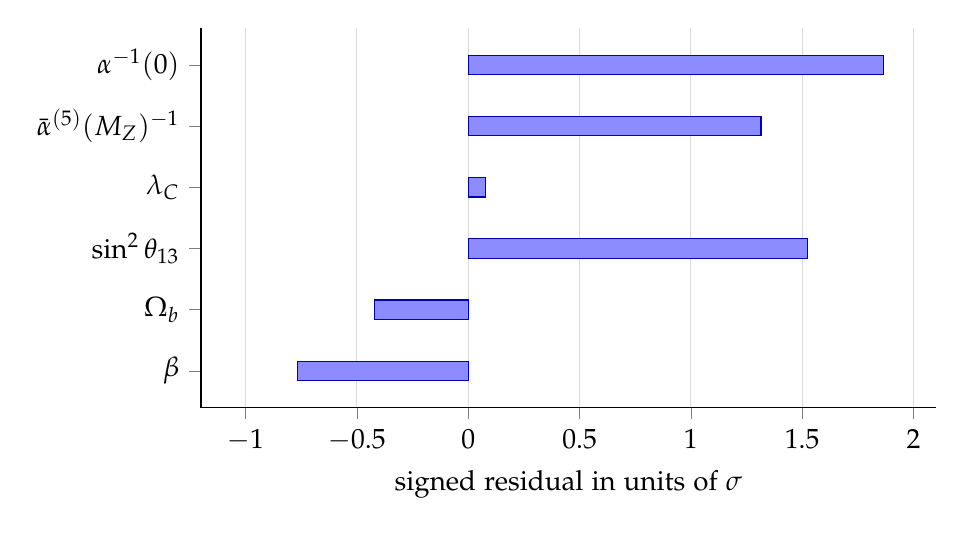
\begin{tikzpicture}
\begin{axis}[
    width=0.9\linewidth,
    height=6.4cm,
    xbar,
    bar width=7pt,
    xmin=-1.2,
    xmax=2.1,
    xlabel={signed residual in units of $\sigma$},
    symbolic y coords={beta,omegab,theta13,lambdac,alphaMZ,alpha0},
    ytick=data,
    yticklabels={$\beta$,$\Omega_b$,$\sin^2\theta_{13}$,$\lambda_C$,$\bar\alpha^{(5)}(M_Z)^{-1}$,$\alpha^{-1}(0)$},
    enlarge y limits=0.12,
    axis x line*=bottom,
    axis y line*=left,
    tick align=outside,
    major grid style={draw=gray!30},
    xmajorgrids=true
]
\addplot[fill=blue!45, draw=blue!70!black] coordinates {
    (-0.768,beta)
    (-0.421,omegab)
    (1.524,theta13)
    (0.078,lambdac)
    (1.315,alphaMZ)
    (1.865,alpha0)
};
\end{axis}
\end{tikzpicture}
\caption{Residual plot for the main intrinsic-observation rows with declared uncertainties.}
\label{fig:residual-plot}
\end{figure}

The principal remaining refinements are therefore specific rather than diffuse:
\begin{itemize}[leftmargin=1.5em, topsep=3pt, itemsep=2pt]
    \item the CKM phase is read from the exact holonomy phase, with only the small-area transport asymptotic kept as a derived expansion,
    \item the nonabelian comparison channels now split into fixed local carrier closure and explicit matching functionals, so the remaining sensitivity is numerical rather than structural,
    \item direct-search interface rows remain pressure tests on the closed branch rather than precision residual rows.
\end{itemize}

\subsection{Falsification matrix}

The present draft does not ask the reader to accept one undifferentiated \enquote{compiler} claim. Each main-text closure statement has a corresponding local or global failure mode, and those failure modes should be readable without first decoding the appendix tables.

The matrix below is therefore intentionally short. It collects only the load-bearing main-paper statements whose failure would break the carrier-first architecture at the theorem level, rather than every downstream benchmark row or optional appendix interface.

\begin{table}[t]
\centering
\small
\begin{tabularx}{\linewidth}{@{}>{\raggedright\arraybackslash}p{0.24\linewidth}YY>{\raggedright\arraybackslash}p{0.13\linewidth}@{}}
\toprule
Statement & What would falsify it & Sector affected & Local or global failure \\
\midrule
Primitive relative spectral dynamics & ill-posed APS domain or no finite admissible spectral action on the retained branch & Hard / closure & global \\
Minimal carrier $E_3\oplus E_2$ & failure to recover the one-family packet or the global quotient from the carrier theorem & Hard & global \\
Topological family closure and $\Oadm=48$ & failure of the topological family theorem to globalize the local count & Closure & local-to-structural \\
Bosonic relative index selecting $\Phi$ & no unique seam-even doublet or an unavoidable extra light triplet & Closure & local \\
local spectral-scale / gravity closure for $\Mpl$ and $\vgeo$ & inability to obtain one common closure for $\Mpl$, $\vgeo$, the Einstein branch, and the $R^2$ branch & Closure & global \\
Transport / strong-CP closure & nonzero determinant phase or an unavoidable $\bar\theta$ counterterm & Closure & local \\
Confinement as admissible word selection & necessity of physical states with $z(w)\neq1$ in the low-energy spectrum & Closure & local \\
Nonperturbative admissible QFT closure & no admissible mass gap or no clustering on the retained branch & Closure & global \\
\bottomrule
\end{tabularx}
\caption{Falsification matrix for the present main-paper claims.}
\label{tab:falsification}
\end{table}

\section{Compiler theorem and intrinsic observation}

\subsection{Compiler chain}

Collecting the admissible reduced datum, primitive reconstruction, the closure theorems from the
admissibility complex, and the intrinsic observation layer, the compiler line is
\begin{equation}
\label{eq:closed-compiler-chain}
\begin{aligned}
\Tmin^{\mathrm{adm}}
&\Rightarrow
\Tprim^{\mathrm{kin}}\\
&\Rightarrow
(E_3\oplus E_2,\ G_{\SM}^{\mathrm{glob}},\ S^+)\\
&\Rightarrow
(\Padm,\ F,\ \Oadm=48,\ \Phi,\ \Mpl,\ \vgeo,\ \nabla_F^\star)\\
&\Rightarrow
x_{\mathrm{core}}^\star\\
&\Rightarrow
\mathcal R_{\mathrm{TOE}}
\;\Rightarrow\;
O_{\mathrm{th}}.
\end{aligned}
\end{equation}
This line is not meant as a slogan. Each arrow is attached either to a hard theorem or to one of
the closure theorems of \Cref{sec:closure-theorems}. In practical finite-threshold computations,
$\mathcal R_{\SM}$ is only the numerical preconditioner used to approximate
$\mathcal R_{\mathrm{TOE}}$.

\subsection{Compiler theorem from the admissibility complex}

\begin{theorem}[Compiler theorem from the admissibility complex]
Assume the admissible reduced datum summarized in \Cref{tab:status-matrix}, together with the
closure theorems of \Cref{sec:closure-theorems} and the conditional closure selection theorem
\Cref{thm:observation-closure}. Then every main-text observable in scope is classified by
exactly one of the following status classes:
\begin{enumerate}[label=(\roman*), leftmargin=1.5em, topsep=3pt, itemsep=2pt]
    \item exact algebraic,
    \item conditional geometric or closure,
    \item matched intrinsic observation,
    \item optional extrapolation.
\end{enumerate}
\end{theorem}

\begin{proof}[Proof sketch]
The proof is compositional. The admissible reduced datum reconstructs the primitive layer. The
carrier theorem then fixes the minimal packet, the global Standard Model quotient, one family
packet, the carrier norm, the abelian index, and the exact electromagnetic closure equation. The
closure layer turns admissibility into an operative selector, fixes the family theorem through the
master closure statement, selects the unique light Higgs mode, closes the local spectral-scale
channel, lifts transport into exact Yukawa and holonomy data on the selected branch, fixes the
hadronic space and the strong-CP/anomaly sector, and reconstructs Lorentzian dynamics, record
observables, and the admissible vacuum. The selected minimizer of
\Cref{thm:observation-closure} then generates the observation functor
$\mathcal R_{\mathrm{TOE}}$, so no extra benchmark ontology remains.
\end{proof}

\subsection{Closure stack and observation layer}

The compiler theorem above is only meaningful if the closure arrows are visibly attached to
concrete input packages, output packages, and output classes. Otherwise the theorem reads like a
slogan instead of a compressed map of the argument.

The following table is therefore the structural companion to the theorem: it records which
objects belong to the exact algebraic layer, which belong to the conditional closure stack, and
which are reported on the matched observation surface.

\begin{table}[t]
\centering
\small
\begin{tabularx}{\linewidth}{@{}>{\raggedright\arraybackslash}p{0.20\linewidth}>{\raggedright\arraybackslash}p{0.18\linewidth}>{\raggedright\arraybackslash}p{0.20\linewidth}YY@{}}
\toprule
Closed statement & Input data & Output package & Output class & Observation role \\
\midrule
Primitive reconstruction from reduced datum & $\Tmin^{\mathrm{adm}}$ & $\Tprim$ & Exact algebraic & fixes the starting dynamics before carrier and closure are unfolded \\
Carrier packet & $\Tprim$ & $E_3\oplus E_2$, $G_{\mathrm{SM}}^{\mathrm{glob}}$, $S^+$, $\bone$ & Exact algebraic & defines the particle-theory kernel \\
Master closure theorem & $D_b$, $Q_{\mathrm{tot}}$, $\Delta_{\mathrm{tot}}$ & $\Padm$, $\APSdom$, $F$, $\mathrm{Hol}(\nabla_F)\subset SU(3)_F$ & Conditional geometric or closure & stabilizes flavor, positivity, and coercivity \\
Geometric and transport closure & $\Padm$, $D_{\mathrm{geo}}$, $\mathcal V_{\mathrm{vac}}$ & $\Phi$, $\Mpl$, $\vgeo$, $Y_f$, $\delta_{\mathrm{ph}}$, $\nabla_F^\star$ & Conditional geometric or closure & fixes mass and gauge source data on the selected branch \\
QCD / vacuum / record closure & $\Asing$, $\Theta$, $\Hrel$, $\Vadm$ & $\Hhad$, $\bar\theta=0$, $\rho^\ast$, $\Arec$, $\Pred$ & Conditional geometric or closure & supplies hadronic, vacuum, and observer sectors \\
Conditional UV Bernstein-cone program & $\Gamma_k$, $\mathcal C_B$ & $\Gamma_\star$ & Conditional geometric or closure & gives the regulator-audited UV program \\
Downstream cosmology module & $\Gamma_\star$, $\mathcal U_\Seam$ & $\Omega_{\mathrm{DM}}$, $\eta_B$, $\Lambda_{\mathrm{obs}}$ & Optional extrapolation & evaluates the cosmology-facing block on the selected branch \\
Conditional core closure selection theorem & $\mathcal E_{\mathrm{core}}(x_{\mathrm{core}})$ on $\mathfrak D_{\mathrm{adm}}$ & $x_{\mathrm{core}}^\star$, $\mathcal R_{\mathrm{TOE}}$, $O_{\mathrm{th}}$ & Matched intrinsic observation & generates the scheme-complete observable map; UV and cosmology are evaluated on, but do not enter, the core selection \\
\bottomrule
\end{tabularx}
\caption{Closure stack and intrinsic observation layer for the present main-paper form.}
\label{tab:proof-obligations}
\end{table}

\section{Conclusion}

\subsection{Closed theorem stack}

TFPT is formulated on the admissible reduced datum
\[
\Tmin^{\mathrm{adm}}=(\mathcal A,\mathcal H,D,J,\Gamma,\inv,\nu)
\]
and reconstructs the primitive layer, the minimal carrier packet, the canonical admissibility
selector, the family bundle, the geometric branch, the selected transport branch and family
holonomy data on the retained admissible branch, the admissible vacuum, the conditional UV
Bernstein-cone program, the downstream cosmology module, and the intrinsic observation functor
$\mathcal R_{\mathrm{TOE}}$.

The closed TFPT chain is therefore
\[
\Tmin^{\mathrm{adm}}
\Rightarrow
\Tprim^{\mathrm{kin}}
\Rightarrow
(E_3\oplus E_2,G_{\mathrm{SM}}^{\mathrm{glob}},S^+)
\Rightarrow
(\Padm,F,g,\sigma,\Phi,\nabla_F^\star)
\Rightarrow
x_{\mathrm{core}}^\star
\Rightarrow
\mathcal R_{\mathrm{TOE}}
\Rightarrow
O_{\mathrm{th}}.
\]
The conditional UV Bernstein-cone program evaluates $\Gamma_\star$ on the selected core branch,
while the downstream cosmology module evaluates
$(\Omega_{\mathrm{DM}},\eta_B,\Lambda_{\mathrm{obs}},\ldots)$ on that same branch without
entering the core selection itself.

\subsection{Intrinsic observation layer}

In the final main-text form there is no residual primitive ontology, no residual closure input
package, no primitive transport datum, no local-only observation theorem, and no operational
benchmark based on asymptotic truncation where an exact invariant exists. The main-text output
surface is organized by four classes: exact algebraic, conditional geometric or closure, matched
intrinsic observation, and optional extrapolation.

The physical observation map is generated by a selected core minimizer
$x_{\mathrm{core}}^\star$ of the core closure functional. The practical finite-threshold map $\mathcal R_{\SM}$ remains only the first
numerical preconditioner for computing $\mathcal R_{\mathrm{TOE}}$, not an extra ontological
layer. The present version therefore absorbs the named upgrade theorems of the bridge manuscript
into one common theorem surface.

\subsection{Optional extrapolations}

Optional arithmetic continuations, appendix-level E$_8$ scale grammar, and horizon semantics are
kept as extrapolations and are not part of the theorem surface itself. They are retained only
where they illuminate downstream interpretations without carrying any main-text proof burden.

\appendix

\section{Technical conventions and data layers}
\label{app:tech}

This appendix collects the technical bookkeeping that supports the carrier-first presentation but would slow the early main-text flow if placed before the carrier theorem.

\subsection{Relative objects}

The adjective \enquote{relative} is used in one fixed sense throughout the paper: every operator or action is compared to a declared reference object.

\begin{table}[t]
\centering
\small
\begin{tabularx}{\linewidth}{@{}>{\raggedright\arraybackslash}p{0.22\linewidth}YY@{}}
\toprule
Relative object & Definition or schematic form & Role \\
\midrule
$D_{\mathrm{rel}}$ & $D-D_{\mathrm{ref}}$ or a specified relative pair $(D,D_{\mathrm{ref}})$ & fermionic comparison operator \\
$S_{\mathrm{rel}}$ & $\tr f(D/\Lambda)-\tr f(D_{\mathrm{ref}}/\Lambda)+\frac{i\pi}{2}\Delta\eta$ & relative spectral action \\
$\Ind_{\mathrm{rel}}$ & APS-type index of a relative pair or superconnection package & carrier and bosonic counting \\
$Z_{\mathrm{rel}}$ & $Z_{\mathrm{adm}}[J,\eta,\bar\eta]/Z_{\mathrm{ref}}[0,0,0]$ & normalized admissible generating functional \\
$\Padm$ & $\operatorname*{s-lim}_{\beta\to\infty}e^{-\beta\Kadm}$; factorized form when the elementary projectors commute & operative admissibility selector on the closed branch \\
$\langle W(C)\rangle_{\mathrm{rel}}$ & Wilson observable after subtraction of the declared reference sector & confinement diagnostics \\
$\mathcal H_{\mathrm{rel}}$ & relative Hamiltonian used in admissible-sector minimization & optional record extension \\
\bottomrule
\end{tabularx}
\caption{Conventions on relative objects.}
\label{tab:relative-objects}
\end{table}

\subsection{Layered datum and admissibility}

\begin{construction}[Layered datum]
The technical bookkeeping behind the manuscript uses four levels:
\[
\Tcore^{\mathrm{kin}}
=
\bigl(
\widetilde M\to M,\ \Seam,\ \inv,\ D_{\mathrm{ref}},\ D_{\mathrm{rel}},\ f,\ \chiseed
\bigr),
\]
\[
\Tker
=
\bigl(
E_3\oplus E_2,\ Y,\ S^+,\ \gamma,\ B,\ G_{\SM}^{\mathrm{glob}},\ \bone(N_{\mathrm{fam}},N_\Phi)
\bigr),
\]
\[
\Tbridge
=
\bigl(
\mathcal R_{\SM},\ \alpha(0),\ M_Z,\ \{m_c,m_b,m_\tau,m_t\}
\bigr),
\]
\[
\Tcomp
=
\left(
\begin{array}{l}
(\mathsf{Adm},\Kadm,\Padm),\ (\chigeo,\mathcal B_{\mathrm{rel}},\mathbb A_{\Seam}),\ (F,T),\\
(U_6,D_y,\mathcal Y_y^{(\varepsilon)},\epsilon_f),\ (Z_{\mathrm{rel}},\Theta,\Hrel,\Vadm),\\
(\Arec,\Aobs,\Pred)
\end{array}
\right).
\]
\end{construction}

Thus $\Tcore^{\mathrm{kin}}$ is the appendix bookkeeping rewrite of the primitive kinematic
scaffold, while $\mathsf{Adm}$ first enters the layered datum only at closure level through
$(\mathsf{Adm},\Kadm,\Padm)$. When an almost-commutative factorization
$\mathcal H\cong L^2(\widetilde M,S)\otimes\Hint$ is chosen, $S$ and $\Hint$ refer to that
factorization and are not additional entries in $\Tcore^{\mathrm{kin}}$.

Conditional horizon and far-downstream E$_8$ data are kept outside this compact layered datum and are introduced only in the dedicated appendix-level extension.

\begin{table}[t]
\centering
\small
\begin{tabularx}{\linewidth}{@{}>{\raggedright\arraybackslash}p{0.12\linewidth}>{\raggedright\arraybackslash}p{0.31\linewidth}>{\raggedright\arraybackslash}p{0.13\linewidth}Y@{}}
\toprule
Level & Objects & Claim role & Function in the present paper \\
\midrule
Core datum & $\widetilde M\to M$, $\Seam$, $\inv$, $D_{\mathrm{ref}}$, $D_{\mathrm{rel}}$, $f$, $\chiseed$ & Reduced datum & minimal kinematic scaffold before carrier data and admissibility closure; $S$ and $\Hint$ refer to a chosen factorization \\
Carrier kernel & $E_3\oplus E_2$, $Y$, $S^+$, $\gamma$, $B$, $G_{\SM}^{\mathrm{glob}}$, $\bone(N_{\mathrm{fam}},N_\Phi)$ & Exact algebraic & rigid particle-theory packet extracted from the core datum \\
Closure data & $(\mathsf{Adm},\Kadm,\Padm)$, $(F,T)$, $(D_{\mathrm{geo}},\chigeo,\mathcal B_{\mathrm{rel}},\mathbb A_{\Seam})$, $(U_6,D_y,\mathcal Y_y^{(\varepsilon)},\epsilon_f)$, $(Z_{\mathrm{rel}},\Theta,\Hrel,\Vadm)$, $(\Arec,\Aobs,\Pred)$ & Conditional geometric or closure & collects the admissibility, family, geometric, transport, OS, record, and vacuum data used by the main closure theorems \\
Observation layer & $\mathcal R_{\mathrm{TOE}}$, $\mathcal R_{\SM}$, $\alpha(0)$, $M_Z$, $\{m_c,m_b,m_\tau,m_t\}$ & Matched intrinsic observation & translates closed compiler outputs into scheme-specified observables, with $\mathcal R_{\SM}$ only the practical numerical preconditioner \\
\bottomrule
\end{tabularx}
\caption{Core datum versus exact algebraic kernel, conditional closure, and matched intrinsic observation structures.}
\label{tab:layered-datum}
\end{table}

\subsection{Symbol guide}

The main text uses a small number of recurrent symbols across different layers. The table below records their first-duty meaning and status class, now including the seam-matching notation introduced in Definition~9.1, so that the manuscript can be read without repeatedly reverse-engineering the bookkeeping.

\begin{table}[t]
\centering
\small
\begin{tabularx}{\linewidth}{@{}>{\raggedright\arraybackslash}p{0.23\linewidth}Y>{\raggedright\arraybackslash}p{0.18\linewidth}@{}}
\toprule
Symbol & First-duty meaning in the paper & Status class \\
\midrule
$\Tprim^{\mathrm{kin}}$ & primitive kinematic scaffold $(\widetilde M\to M,\Seam,\inv,D_{\mathrm{ref}},D_{\mathrm{rel}},f,\chiseed)$; when an almost-commutative factorization is chosen, $S$ and $\Hint$ refer to that choice and are not additional reconstruction outputs & Exact algebraic \\
$\chiseed$ & primitive seam-even scalar response reconstructed on the primitive layer before geometric reconstruction & Exact algebraic \\
$\sigma,\ \chigeo$ & local Weyl field and derived local spectral scale $\chigeo=\Lambda e^\sigma$ on the geometric branch & Conditional geometric or closure \\
$\APSdom,\ \APSfam$ & elliptic APS domain for primitive well-posedness and the canonically induced family-pairing data on the closed branch & Conditional geometric or closure \\
$\Tmin$ & reduced theorem-path datum $(\mathcal A,\mathcal H,D,J,\Gamma,\inv,\nu)$ with positive spectral measure $\nu$ & Reduced datum \\
$E_3\oplus E_2$ & minimal carrier split into color and weak sectors & Exact algebraic \\
$\bone(N_{\mathrm{fam}},N_\Phi)$ & carrier-side abelian coefficient function before canonical branch evaluation & Exact algebraic \\
$\mathsf{Adm},\Kadm,\Padm$ & admissibility predicate, positive constraint operator, and operative selector on the admissible branch & Conditional geometric or closure \\
$F,\Oadm$ & topological family space and occupancy count after family closure; $\Oadm$ later feeds the observation reading of $\deltatop$ & Conditional geometric or closure \\
$\mathcal I_{41}$ & weighted integrity index $10\,\bone=\Omega_{\mathrm{occ}}\gamma+N_\Phi$ on the canonical branch & Exact algebraic \\
$\delta_{\mathrm{ph}}$ & transport stationary point on the $C_6$ hexagon used on the selected branch & Conditional geometric or closure \\
$\mathcal R_{\SM}$ & practical finite-threshold numerical preconditioner for the scheme-specified observation map & Matched intrinsic observation support \\
$\mathcal S_{\mathrm{int}},\mathcal S_{\mathrm{obs}}$ & intrinsic closure surface and observation surface $\mathcal R_{\mathrm{TOE}}(\mathcal S_{\mathrm{int}})$ for the compiler interface & Conditional closure / matched intrinsic observation \\
$\hat m_f,\ m_f^{\mathrm{obs}}$ & internal compiler source masses and their observation-surface images after matching & Conditional closure / matched intrinsic observation \\
$M_\Sigma,\ g_\Sigma$ & seam matching scale read from the first positive seam boundary mode and the gauge coupling evaluated there & Conditional closure / matched intrinsic observation \\
$Q_\Theta$ & determinant-sector involution entering admissibility and the projector $P_\Theta$ & Conditional geometric or closure \\
$\mathcal C_\Sigma$ & sheet-CP symmetry operator $CP\circ\inv$ on the admissible branch & Conditional geometric or closure \\
$T$ & transport generator on the family / holonomy side & Conditional geometric or closure \\
$\mathfrak C_\Sigma$ & seam cycle data used by the matching and holonomy packages & Conditional geometric or closure \\
$\wspin$ & spin holonomy weight entering the geometric package & Conditional geometric or closure \\
$\Arec,\Aobs,\Pred$ & stable record algebra, observer algebra, and prediction map on the admissible sector & Conditional geometric or closure \\
\bottomrule
\end{tabularx}
\caption{Symbol guide with first-duty meaning and status class.}
\label{tab:symbol-guide}
\end{table}

\begin{definition}[Admissibility predicate and selector]
In the present paper $\mathsf{Adm}$ denotes a predicate on relative sectors, and $\Padm$ denotes its operator realization on the retained closed branch. We write $\mathsf{Adm}(X)=1$ precisely when:
\begin{enumerate}[label=(\arabic*), leftmargin=1.5em, topsep=3pt, itemsep=2pt]
    \item $X$ lies in the declared domain of the relative operator pair,
    \item the associated relative action or index density is finite after reference subtraction,
    \item the required seam-evenness condition is satisfied,
    \item colored sectors satisfy center neutrality when a hadronic interpretation is intended,
    \item gap-stable transport positivity and the declared closure conditions hold in those sectors used for observable or transport statements.
\end{enumerate}
On those sectors, the selector language and the predicate language are identified by
\[
\mathsf{Adm}(X)=1
\quad\Longleftrightarrow\quad
\Padm X=X.
\]
\end{definition}

\begin{remark}[Operator realization of admissibility]
If one wants an operator language rather than a predicate language, the natural positive generator is $\Kadm$ and its commuting-factor realization is
\[
P_{\mathrm{adm}}=P_{\Seam,+}\,P_{\mathrm{sing}}\,P_{\Theta}\,P_{\mathrm{gap}},
\]
where the factors act on the commuting seam, color, determinant, and transport sectors of the admissible Hilbert-space decomposition. Here $P_{\Seam,+}$ projects to seam-even sectors, $P_{\mathrm{sing}}$ to center-neutral singlets when a hadronic interpretation is intended, $P_{\Theta}$ encodes the declared sheet / determinant selection, and $P_{\mathrm{gap}}$ imposes the transport-side positivity or gap condition. The main text defines $\Padm$ as the zero-temperature projector of $\Kadm$; the appendix records the explicit factorization available on the commuting retained branch.
\end{remark}

\section{Constants atlas and downstream scale grammar}
\label{app:constants}

This appendix collects material that is useful for internal compression but should not dominate the main-text scope of explicit claims.

\subsection{Global rotation angle and constants atlas}

The seam loop is assumed to carry one unit of spectral flow,
\[
U_{\Seam}(\theta)=e^{i\theta},
\qquad
\SF(U_{\Seam})=1,
\qquad
\Delta_{\Seam}=2\pi.
\]
Because the spin lift closes only after $4\pi$, the normalized rotation modulus is
\[
\atheta=\frac{\theta}{4\pi}.
\]
The cascade in \Cref{fig:constant-cascade} is kept here as technical bookkeeping rather than as an early main-text dependency graphic.

\begin{figure}[t]
\centering
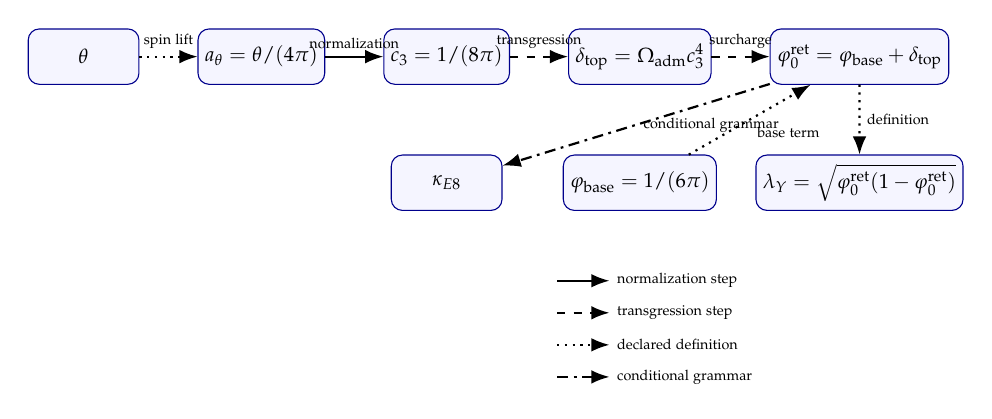
\begin{tikzpicture}[
    scale=0.74,
    transform shape,
    >=Latex,
    node distance=1.2cm and 1.0cm,
    box/.style={draw=blue!55!black, rounded corners, fill=blue!4, align=center, minimum width=1.9cm, minimum height=0.95cm},
    hardedge/.style={->, thick},
    bridgeedge/.style={->, dashed, thick},
    definedge/.style={->, dotted, thick},
    optedge/.style={->, dash pattern=on 4pt off 2pt on 1pt off 2pt, thick}
]
\node[box] (theta) {$\theta$};
\node[box, right=of theta] (a) {$\atheta=\theta/(4\pi)$};
\node[box, right=of a] (c3) {$\cthree=1/(8\pi)$};
\node[box, right=of c3] (delta) {$\deltatop=\Oadm \cthree^4$};
\node[box, right=of delta] (phi0) {$\phiz=\phibase+\deltatop$};
\node[box, below=of delta] (phibase) {$\phibase=1/(6\pi)$};
\node[box, below=of phi0] (lambda) {$\lambdaY=\sqrt{\phiz(1-\phiz)}$};
\node[box, below=of c3] (e8) {$\kappa_{E8}$};
\draw[definedge] (theta) -- node[above, font=\scriptsize] {spin lift} (a);
\draw[hardedge] (a) -- node[above, font=\scriptsize] {normalization} (c3);
\draw[bridgeedge] (c3) -- node[above, font=\scriptsize] {transgression} (delta);
\draw[definedge] (phibase) -- node[below right, font=\scriptsize] {base term} (phi0);
\draw[bridgeedge] (delta) -- node[above, font=\scriptsize] {surcharge} (phi0);
\draw[definedge] (phi0) -- node[right, font=\scriptsize] {definition} (lambda);
\draw[optedge] (phi0) -- node[right, font=\scriptsize] {conditional grammar} (e8);
\coordinate (legA) at ($(phibase.south west)+(-0.1,-1.2)$);
\draw[hardedge] (legA) -- ++(0.9,0) node[right, black, font=\scriptsize] {normalization step};
\coordinate (legB) at ($(legA)+(0,-0.55)$);
\draw[bridgeedge] (legB) -- ++(0.9,0) node[right, black, font=\scriptsize] {transgression step};
\coordinate (legC) at ($(legB)+(0,-0.55)$);
\draw[definedge] (legC) -- ++(0.9,0) node[right, black, font=\scriptsize] {declared definition};
\coordinate (legD) at ($(legC)+(0,-0.55)$);
\draw[optedge] (legD) -- ++(0.9,0) node[right, black, font=\scriptsize] {conditional grammar};
\end{tikzpicture}
\caption{Constant cascade used for technical bookkeeping, shown in the occupancy-reinterpretation form for $\deltatop$. Arrow styles encode algebraic role rather than claim status: normalization, transgression, declared definition, and conditional downstream grammar.}
\label{fig:constant-cascade}
\end{figure}

Here the arrow $\atheta\to\cthree$ records a normalization convention internal to the present setup, not an independently proved theorem beyond the declared seam and spin-lift normalization.

\begin{table}[t]
\centering
\scriptsize
\setlength{\tabcolsep}{3pt}
\begin{tabularx}{\linewidth}{@{}>{\raggedright\arraybackslash}p{0.10\linewidth}>{\raggedright\arraybackslash}p{0.18\linewidth}>{\raggedright\arraybackslash}p{0.12\linewidth}>{\raggedright\arraybackslash}p{0.11\linewidth}YY@{}}
\toprule
Symbol & Definition & Compiler role & First origin & Reappears in & Physical meaning \\
\midrule
$\theta$ & seam-loop angle & core datum & seam data & $\atheta$ & geometric rotation variable \\
$\atheta$ & $\theta/(4\pi)$ & hard normalization & spin lift & $\cthree$, phase grammar & normalized cover rotation \\
$\cthree$ & $1/(8\pi)$ & hard kernel constant & seam normalization & $\deltatop$, $\beta$, $\sigma$ & seam normalization constant \\
$\phibase$ & $1/(6\pi)$ & hard kernel constant & carrier geometry & $\phiz$ & base opening \\
$\deltatop$ & $\frac{3}{256\pi^4}$; observation reading $\Oadm\cthree^4$ & hard kernel value with occupancy reinterpretation & retained numerical kernel & $\phiz$, $\delta_2$ & topological surcharge \\
$\phiz$ & $\frac{1}{6\pi}+\frac{3}{256\pi^4}$ & retained canonical seed & retained numerical kernel & $\lambdaY$, $\beta$, flavor & minimal nontrivial opening \\
$\gamma$ & $\tr_EY^2=5/6$ & hard kernel invariant & carrier packet & $\kappa_{E8}$, $\delta_2$ & carrier norm \\
$B$ & $\rank E_3/\rank E_2=3/2$ & hard kernel invariant & carrier packet & $\delta_2$ & carrier rank ratio \\
$\Oadm$ & $3\times16=48$ & closure quantity with bridge reinterpretation & APS family closure & $\deltatop$ & admissible chiral-state count on the family-closed branch \\
$\bone$ & $\frac43N_{\mathrm{fam}}+\frac1{10}N_\Phi$ & hard kernel output & abelian index & benchmark map & hypercharge trace coefficient \\
$\kappa_{E8}$ & $\gamma/\ln(248/60)$ & conditional grammar & Appendix~\ref{app:constants} & scale ladder & optional scale spacing \\
\bottomrule
\end{tabularx}
\caption{Constants atlas for the present manuscript.}
\label{tab:constants-atlas}
\end{table}

\subsection{\texorpdfstring{E$_8$}{E8} as downstream scale grammar}

In the present paper E$_8$ is not used as a primitive cause. The retained parameter is
\[
\kappa_{E8}:=\frac{\gamma}{\ln(248/60)}=\frac{5/6}{\ln(248/60)}.
\]
On the retained branch this means
\[
\begin{aligned}
\kappa_{E8}&\approx \num{0.58723},
&
f_a&\approx \num{8.86e10}\,\mathrm{GeV},
\\
m_a&\approx \num{65.19}\,\mu\mathrm{eV},
&
\nu_a&\approx \num{15.764}\,\mathrm{GHz}.
\end{aligned}
\]
The intended reading is a downstream scale grammar:
\begin{itemize}[leftmargin=1.5em, topsep=3pt, itemsep=2pt]
    \item the carrier packet fixes $\gamma=5/6$,
    \item $\kappa_{E8}$ then defines an optional ladder parameter,
    \item the ladder is allowed to organize scale spacing,
    \item but it does not replace the carrier theorem or the seam data.
\end{itemize}
In the fuller appendix-level grammar one may package a downstream block scale as
\[
X(n,r,I_1)=\frac{\Mplunred}{8}\,\sin^2\theta_{13}
\left(\frac{60-2n}{60}\right)^{\kappa_{E8}}
e^{-(8-r)/64}e^{-12\pi I_1},
\]
where $n$ is the ladder stage, $r$ a mild block-multiplicity label, and $I_1$ the dominant block trace. This makes the reading discipline explicit: the stage index orders the ladder, the trace controls most of the exponential suppression, and the extra block label only refines the scale. The denominator $64$ is part of that downstream grammar and is not interpreted here as a Hilbert-space dimension, state count, or hidden spinor multiplicity. E$_8$ is therefore a downstream scale grammar, not a universal mass formula.

\subsection{Full stage atlas}

The full real-domain atlas up to $n=29$ extends the main-text robust table with restricted-scan candidates and IR tail conjectures. Rows are classified as \emph{robust} (restrictive grammar, unambiguous target), \emph{restricted-scan} (plausible but less constrained), or \emph{tail conjecture} (new trace class $I_1\in\{\frac{11}{12},\frac{7}{6}\}$ not yet derived from block structure).

\begin{table}[H]
\centering
\scriptsize
\setlength{\tabcolsep}{2pt}
\begin{tabularx}{\linewidth}{@{}>{\centering\arraybackslash}p{0.035\linewidth}>{\centering\arraybackslash}p{0.035\linewidth}>{\raggedright\arraybackslash}p{0.065\linewidth}>{\raggedleft\arraybackslash}p{0.12\linewidth}>{\raggedleft\arraybackslash}p{0.12\linewidth}>{\raggedright\arraybackslash}p{0.09\linewidth}>{\raggedright\arraybackslash}p{0.17\linewidth}Y@{}}
\toprule
$n$ & $r$ & $I_1$ & $X$ (GeV) & Target & Residual & Identification & Class \\
\midrule
$3$ & $8$ & $1/2$ & $\num{2.159e8}$ & $\num{2.160e8}$ & $0.06\%$ & $\mu_{\cthree}$ RG crossing & robust \\
$5$ & $5$ & $1/12$ & $\num{1.307e15}$ & $\num{1.31e15}$ & $0.2\%$ & seesaw $M_R$ & robust \\
$6$ & $6$ & $1$ & $\num{1.272}$ & $\num{1.27}$ & $0.2\%$ & charm band & restricted-scan \\
$8$ & $1$ & $17/16$ & $\num{0.1059}$ & $\num{0.10566}$ & $0.2\%$ & muon band & restricted-scan \\
$10$ & $1$ & $1/3$ & $\num{8.826e10}$ & direct search & --- & PQ scale $f_a$ & robust \\
$12$ & $2$ & $41/48$ & $\num{246.35}$ & $\num{246.22}$ & $0.05\%$ & EW reference scale & robust \\
$14$ & $4$ & $17/16$ & $\num{0.0921}$ & $\num{0.0927}$ & $0.6\%$ & $f_\pi$ band & robust \\
$15$ & $4$ & $1$ & $\num{0.935}$ & $\num{0.938}$ & $0.3\%$ & hadron anchor & robust \\
$21$ & $4$ & $1/6$ & $\num{3.051e13}$ & $\num{3.06e13}$ & $0.3\%$ & inflation $M$ & robust \\
$21$ & $5$ & $41/48$ & $\num{171.8}$ & $\num{172.6}$ & $0.4\%$ & top quark & robust \\
$24$ & $7$ & $5/8$ & $\num{7.895e5}$ & $\num{7.920e5}$ & $0.3\%$ & $\mu_{\phiz}$ RG crossing & robust \\
$25$ & $5$ & $1$ & $\num{0.498}$ & $\num{0.498}$ & $0.0\%$ & kaon band & robust \\
$25$ & $7$ & $41/48$ & $\num{125.5}$ & $\num{125.25}$ & $0.2\%$ & Higgs mass & robust \\
$26$ & $2$ & $1$ & $\num{0.417}$ & $\num{0.42}$ & $0.7\%$ & $\sqrt{\sigma}$ confinement & robust \\
$27$ & $6$ & $41/48$ & $\num{91.6}$ & $\num{91.19}$ & $0.4\%$ & $Z$ boson & restricted-scan \\
$28$ & $1$ & $7/6$ & $\num{5.105e-4}$ & $\num{5.110e-4}$ & $0.1\%$ & electron & tail conjecture \\
$29$ & $1$ & $11/12$ & $\num{4.210}$ & $\num{4.18}$ & $0.7\%$ & bottom quark & tail conjecture \\
\bottomrule
\end{tabularx}
\caption{Full E$_8$ stage atlas on the canonical branch up to the real-domain boundary $n=29$.}
\label{tab:e8-full-atlas}
\end{table}

\subsection{Compression identities on the minimal branch}

The main-text compression identities are developed in the dedicated section on compression identities and carrier exclusion. This appendix subsection collects additional arithmetic continuations and the compression chain summary.

\begin{remark}[Abelian package from occupancy and carrier norm]
On the canonical branch,
\[
\Oadm\gamma=48\cdot\frac56=40.
\]
Thus the characteristic coefficient $41$ is compressed to
\[
41=\Oadm\gamma+1=40+1,
\]
that is, fermionic occupancy trace plus one light Higgs doublet contribution.
Writing $b_Y:=5\bone/3$ for the usual hypercharge-normalized coefficient and using the block-index relation $k_B=\frac32 I_1(B)$ to define $I_1^{\mathrm{EW}}:=\frac{5}{24}\bone$ and $k_{\mathrm{EW}}:=\frac{5}{16}\bone$, one obtains the unified chain
\begin{equation}
\label{eq:41-chain}
48\,I_1^{\mathrm{EW}}
=32\,k_{\mathrm{EW}}
=10\,\bone
=\Oadm\gamma+1
=41.
\end{equation}
Equivalently,
\[
I_1^{\mathrm{EW}}=\frac{41}{48},
\qquad
k_{\mathrm{EW}}=\frac{41}{32},
\qquad
\bone=\frac{41}{10},
\qquad
b_Y=\frac{41}{6}.
\]
This is an algebraic signature rather than an accidental coincidence: the same integer $41$ appears simultaneously as electroweak block trace, E$_8$ exponent, UV hypercharge trace, and carrier occupancy times norm plus one.
\end{remark}

\begin{remark}[Rank lock and single-seed compression: main-text reference]
The rank-lock identity $2^{g-3}=g-1\Rightarrow g=5$ is proved as \Cref{prop:rank-lock} in the main text.
The single-seed compression and the Cabibbo inversion $\phiz=\frac12(1-\sqrt{1-4\lambda_C^2})$ with all derived inter-observable relations are given in \Cref{eq:cabibbo-inversion,eq:lambda-c-master}. The carrier exclusion theorems for wrong discrete worlds are in \Cref{thm:carrier-exclusion}.
\end{remark}

\subsection{Optional arithmetic continuations}

The next relations mix the main-text carrier with optional appendix-level E$_8$, inflation, or geometric notation. They are useful compression patterns, but their interpretation should remain conditional or conjectural.

\begin{remark}[60, 48, and \texorpdfstring{$5/4$}{5/4} on the optional ladder]
If the optional scale ladder is started at $D_1=60$, then
\[
\frac{D_1}{\Oadm}=\frac{60}{48}=\frac54=B\gamma.
\]
On the minimal branch one may also write the same number as
\[
\frac54=\frac{\gcar}{\gcar-1}\qquad (\gcar=5).
\]
This compresses the E$_8$ start index, the admissible chiral count, the mirror factor, and the two-defect coefficient to the same rational factor.
\end{remark}

\begin{remark}[Factorization of the two defect coefficient and arithmetic completion of $48$ and $60$]\label{rem:defect-factorization-gcd-lcm}
From the main text identity
\[
\delta_2=\frac{5}{4}\,\deltatop^2,
\qquad
\deltatop=\Oadm\cthree^4,
\]
one obtains
\[
\delta_2=2880\,\cthree^8.
\]
On the canonical branch this factor admits the exact arithmetic decompositions
\[
2880=\Dstart\Oadm=60\cdot48,
\qquad
2880=|R(E_8)|\,\dim \mathfrak g_{\SM}=240\cdot12.
\]
The same pair $(\Oadm,\Dstart)=(48,60)$ also satisfies
\[
\gcd(\Oadm,\Dstart)
=
12
=
\dim \mathfrak g_{\SM},
\]
and
\[
\operatorname{lcm}(\Oadm,\Dstart)
=
\frac{\Oadm\Dstart}
{\gcd(\Oadm,\Dstart)}
=
240
=
|R(E_8)|.
\]
So the gauge algebra dimension is the common divisor of the carrier-side counting pair, while the E$_8$ root count is its least common multiple. The arithmetic identities are exact. Here the value $12$ is the Lie-algebra dimension
\[
\dim\mathfrak g_{\SM}=8+3+1,
\]
not a derivation from a discrete permutation group of order $12$; at most the $3+2$ split carries such a discrete shadow. Their E$_8$ reading remains appendix level and conditional in the sense fixed elsewhere in the manuscript.
\end{remark}

\begin{conjecture}[E$_8$ root-count reading]
On the same optional branch,
\[
|R(E_8)|=248-8=240=5\cdot48=5\,\Oadm.
\]
This suggests that the E$_8$ root count may be read as a fivefold unfolding of the admissible chiral packet, although that interpretation is not used as a main-text theorem.
\end{conjecture}

\begin{remark}[Reactor seed of the optional scale ladder]
If one writes the optional ladder as
\[
\varphi_n=\phiz e^{-\gamma}\left(\frac{D_n}{D_1}\right)^{\kappa_{E8}},
\qquad
D_n=60-2n,
\]
then the start value is precisely the reactor-angle seed,
\[
\varphi_n=\sin^2\theta_{13}\left(\frac{D_n}{D_1}\right)^{\kappa_{E8}}.
\]
Thus the appendix-level ladder may be read as a discrete continuation of the same seed that controls $\theta_{13}$.
\end{remark}

\begin{remark}[Conditional inflation-side compression]
If one supplements the appendix with the conditional Starobinsky-side relations
\[
A_s=\frac{N^2}{24\pi^2}\left(\frac{M}{\Mpl}\right)^2,
\qquad
\frac{M}{\Mpl}=\sqrt{8\pi}\,\cthree^4,
\]
then on the minimal branch
\[
A_s=\frac{N^2}{3\pi}\cthree^8=\frac{N^2}{8640\pi}\,\delta_2,
\]
and also
\[
\frac{M}{\Mpl}=\frac{\sqrt{8\pi}}{\Oadm}\,\deltatop.
\]
This is recorded only as an appendix-level compression identity because inflation is outside the present main-text claim surface.
\end{remark}

\begin{remark}[Dyonic intercept and the $\alpha$ kernel]
From the dyonic appendix the local astrophysical $\beta$ function reads
\[
\beta_{\mathrm{BH}}(r)=\frac{Q_eQ_m}{256\pi^4 r^2}=\frac{\deltatop}{3}\frac{Q_eQ_m}{r^2}=16\cthree^4\frac{Q_eQ_m}{r^2}.
\]
This is a cross-link between the EHT intercept channel and the $\alpha$ kernel: the same topological coefficient $\deltatop=48\cthree^4$ that pushes $\alpha$ into the precision zone also controls the local dyonic $\beta$ function. The local and cosmological sectors are therefore not two loose motifs but the same coefficient in two projections.
\end{remark}

\begin{remark}[Conditional occupancy route to gravity]
If the relative Einstein term is of the form
\[
S_{\mathrm{EH}}^{\mathrm{rel}}
=
\frac{\chigeo^2}{192\pi^2}\tr_{\mathcal H_{\mathrm{ch}}}\mathbf 1
\int d^4x\sqrt{-g}\,R,
\]
and if the family bridge identifies
\[
\tr_{\mathcal H_{\mathrm{ch}}}\mathbf 1=\Oadm=48,
\]
then
\[
\Mpl^2=\frac{\chigeozero^2}{2\pi^2}.
\]
This is the occupancy-to-gravity route alluded to in the main text.
\end{remark}

\begin{remark}[Compression chain]
The appendix-level compression pattern may therefore be summarized as
\[
Y \leftrightarrow \inv,
\qquad
\gamma=\frac56,
\qquad
B\gamma=\frac54,
\qquad
\frac{D_1}{\Oadm}=\frac54,
\qquad
|R(E_8)|=5\,\Oadm,
\]
\[
\bone=\frac{\Oadm\gamma+1}{10},
\qquad
\Omega_b+\beta_{\mathrm{rad}}=\phiz,
\qquad
A_s=\frac{N^2}{8640\pi}\,\delta_2
\quad
\text{(conditional inflation-side import)}.
\]
\end{remark}

\subsection{Conditional minimal-parameter picture}

The next package is stronger but also more conditional. It assumes that the carrier rank, family multiplicity, and seam normalization are all read as closed rather than only partially inherited.

\begin{principle}[Conditional minimal-parameter compression]
Assume the canonical branch
\[
\gcar:=\rank E=5,
\qquad
N_{\mathrm{fam}}=3,
\qquad
\cthree=\frac{1}{8\pi}.
\]
Then the numerical kernel may be rewritten almost entirely in terms of
\[
(\pi,\gcar,N_{\mathrm{fam}})=(\pi,5,3).
\]
Indeed, on this branch one has
\[
\gamma=\frac56=\frac{\gcar}{\gcar+1},
\qquad
\dim S^+=2^{\gcar-1},
\qquad
\Oadm=N_{\mathrm{fam}}2^{\gcar-1}=48,
\]
\[
\phibase=\frac{1-\gamma}{\pi}=\frac{1}{(\gcar+1)\pi},
\qquad
\deltatop=\Oadm\,\cthree^4,
\qquad
\delta_2=\Dstart\,\Oadm\,\cthree^8,
\]
with
\[
\Dstart=\gcar\,\dim\mathfrak g_{\SM}=5\cdot 12=60,
\qquad
\Oadm=(\gcar-1)\dim\mathfrak g_{\SM}=4\cdot 12=48.
\]
\end{principle}

\begin{remark}[Compressed dependency chain]
Under the same conditional closure, the appendix-level numerical chain reads
\[
(\widetilde M\to M,\Seam,\inv,\chiseed)
\Longrightarrow
E_3\oplus E_2
\Longrightarrow
Y \leftrightarrow \inv
\Longrightarrow
S(U(3)\times U(2))
\Longrightarrow
S^+,
\]
\[
\Longrightarrow
N_{\mathrm{fam}}=3
\Longrightarrow
\Oadm=48
\Longrightarrow
(\deltatop,\delta_2,\phiz)
\Longrightarrow
(\alpha,\lambda_C,\beta_{\mathrm{rad}},\Omega_b,\sin^2\theta_{13}),
\]
with the optional E$_8$, inflationary, and gravity-side sectors then read as downstream continuations of the same compressed core.
\end{remark}

\section{Relative APS and superconnection setup}
\label{app:aps}

The geometric completion uses APS-type relative data \cite{aps1975}. In practice this means:
\begin{itemize}[leftmargin=1.5em, topsep=3pt, itemsep=2pt]
    \item one works with a declared pair $(D,D_{\mathrm{ref}})$ rather than a single unanchored operator,
    \item boundary conditions on the seam $\Seam$ are part of the definition of the relative index,
    \item the $\eta$-term keeps track of the residual spectral asymmetry,
    \item the superconnection package is used in the same spirit as the spectral-action tradition \cite{chamseddineConnes1997}, but here always with an explicit reference subtraction.
\end{itemize}

This appendix now serves as the proof motor for the geometric reconstruction statements in the main text: its role is to make the common reference structure explicit enough that the reconstruction theorem and the local spectral-scale branch are not left hanging on a slogan.

\section{Relative reflection positivity with fermions}
\label{app:os-fermions}

\subsection{Normalized quotient form}

The relative Euclidean theory used in the main closure section is not interpreted as a difference of measures. Instead it is organized as the normalized quotient
\[
Z_{\mathrm{rel}}[J,\eta,\bar\eta]
=
\frac{Z_{\mathrm{adm}}[J,\eta,\bar\eta]}{Z_{\mathrm{ref}}[0,0,0]}.
\]
Because the denominator is source independent on the admissible sector, the reference theory acts only as a fixed normalizer and does not interfere with reflection positivity.

\subsection{Bosonic and fermionic positivity on \texorpdfstring{$\Padm$}{Padm}}

The commutation relations
\[
[\Theta,P_\Theta]=0,
\qquad
\Theta\Padm=\Padm\Theta
\]
ensure that reflection preserves the admissible subspace. The bosonic part then follows the standard Markov / reflection-stable Osterwalder--Schrader argument on admissible observables. For fermions, the admissible CAR kernel may be written as a reflected quadratic form; equivalently one may express the same condition as positivity of the associated Pfaffian structure on the admissible sector. Hence for every admissible observable $O$ supported in $\tau>0$,
\[
\langle \Theta O,O\rangle_{\mathrm{rel}}
=
\frac{1}{Z_{\mathrm{ref}}[0,0,0]}
\langle \Theta O,O\rangle_{\mathrm{adm}}
\ge 0.
\]
This appendix section is the mechanism behind \Cref{lem:admissible-reflection-positivity,thm:reflection-positivity-admissible,thm:lorentzian-reconstruction}; it is recorded here so that the main-text reconstruction theorem is not supported only by a one-line axiom call.

\section{Yukawa kernels and positivity lemmas}
\label{app:yukawa}

This appendix is the proof motor for the transport positivity, strong-CP protection, and bounded-residual statements used in the main text. The transport program is based on the regularized kernel
\[
\mathcal Y_f^{(\varepsilon)}=(D_f^\dagger D_f+\varepsilon^2)^{-1}.
\]
Three remarks are important.
\begin{enumerate}[leftmargin=1.5em, topsep=3pt, itemsep=3pt]
    \item The regulator $\varepsilon$ is not optional: without it the kernel becomes ill-defined exactly where the admissibility question is most delicate.
    \item Positivity of the kernel belongs to the admissibility-closure layer rather than to the hard carrier kernel. The main text closes it through the finite hexagon gap and the lift to the full admissibility-projected operator; this appendix records the transport-side mechanism behind that closure.
    \item Residual prefactors $\Lambda_{f,j}$ are bounded holonomy data inside the transport theorem. They must remain visible and must not be rhetorically hidden as if the mass map were diagonal without residual transport structure.
\end{enumerate}

\begin{remark}[Positive-kernel determinant route to strong CP]
If the physical mass map is written in the polar form
\[
M_f=U_{f,L}H_fU_{f,R}^\dagger,
\qquad
H_f>0,
\qquad
U_{f,L},U_{f,R}\in SU(3)_F,
\]
with $H_f$ induced by the positive transport kernel $\mathcal Y_f^{(\varepsilon)}$, then the induced determinant phase vanishes:
\[
\arg\det M_f=0.
\]
At the same time weak CP may survive through
\[
V_{\mathrm{CKM}}=U_{u,L}^\dagger U_{d,L}.
\]
Combined with the sheet-CP symmetry protection of $\theta_{\mathrm{sheet}}$ in the relative action, this is the algebraic core of the strong-CP theorem stated in the main text. The role of the appendix remark is to display the polar-decomposition mechanics behind that theorem, not to reopen its status.
\end{remark}

\subsection{Optional strong-coupling sharpening}

As an appendix-level sharpening of the closed confinement theorem, one may further require the
admissible center-neutral Wilson functional to obey strong-coupling dominance. On that optional
route the relative Wilson loop satisfies
\[
\langle W(C)\rangle_{\mathrm{rel}}
\le
\exp[-\sigma A_{\min}(C)],
\qquad
\sigma=\cthree^2\chi_{\QCD}^2,
\]
and the physical Hilbert space contains no color-nonsinglet asymptotic states. This statement is
kept in the appendix so that the main theorem surface does not depend on an extra strong-coupling
sharpening beyond the closed admissible hadronic sector.

\section{Information-theoretic and cut-and-project readings}
\label{app:info-readings}

This appendix collects interpretive notes that help organize the algebraic structure of the carrier-first compiler. When an exact algebraic statement appears below, it refers back to a main-text proposition; the appendix itself does not upgrade any status label beyond the declared hard / closure / benchmark / conditional discipline.

\subsection{Integrity-index overdetermination of the canonical branch}

The canonical $41$-chain admits a compact integrity-table reading:

\begin{table}[H]
\centering
\small
\begin{tabularx}{\linewidth}{@{}>{\raggedright\arraybackslash}p{0.26\linewidth}>{\raggedleft\arraybackslash}p{0.12\linewidth}Y@{}}
\toprule
Layer & Value & Role \\
\midrule
Electroweak trace block $48\,I_1^{\mathrm{EW}}$ & $41$ & retained electroweak trace packet \\
Block exponent $32\,k_{\mathrm{EW}}$ & $41$ & E$_8$-side compression datum \\
UV hypercharge coefficient $10\,b_1$ & $41$ & one-loop electroweak closure datum \\
Occupancy-weighted carrier norm $\Oadm\gamma+1$ & $41$ & carrier / family compression identity \\
\bottomrule
\end{tabularx}
\caption{Integrity-index overdetermination of the canonical branch. The common integer is read as an algebraic integrity marker, not as a cryptographic statement.}
\label{tab:checksum-41}
\end{table}

The value of this table is structural rather than rhetorical: four independently defined layers collapse onto one integer on the retained branch. This is exactly the sense in which the branch carries the integrity index $\mathcal I_{41}$.

\subsection{Seed variance and surprisal readings}

The bridge identities also admit a disciplined probabilistic reading. Since
\[
\lambda_C^2=\phiz(1-\phiz),
\]
the Cabibbo scale is exactly the standard-deviation scale of a Bernoulli variable with success probability $p=\phiz$:
\[
\lambda_C=\sqrt{p(1-p)}.
\]
Equivalently, the Fisher information of the Bernoulli family is
\[
I(p)=\frac{1}{p(1-p)}=\frac{1}{\lambda_C^2},
\]
so the Cabibbo bridge measures the inverse square-root Fisher scale of the retained seed. This is the precise information-theoretic statement. The present paper does \emph{not} identify $\lambda_C$ itself with Fisher information or with a Bures distance.

Likewise, whenever the electromagnetic closure is written with
\[
\ln\!\bigl((\phiz)^{-1}\bigr),
\]
the exact probabilistic reading is the surprisal of the seed event. That term should not be called the Shannon entropy of the full Bernoulli distribution, which would instead be
\[
H(\phiz)
=
-\phiz\ln\phiz-(1-\phiz)\ln(1-\phiz).
\]
Finally, the neutrino bridge relation
\[
\sin^2\theta_{13}=\phiz e^{-\gamma}
\]
is naturally described as Boltzmann-like weighting by the carrier norm $\gamma$, but the present draft does not define a full thermodynamic partition function at that point. These readings are therefore organizational interpretations of already established formulas, not new closure theorems.

\subsection{Exact parity-code and information-compression reading}

The strongest information-theoretic statement is no longer a loose analogy. By \Cref{prop:parity-code-family}, the one-family packet is exactly the even-parity subspace on five occupation bits,
\[
S^+
\cong
\mathrm{span}\Bigl\{|x\rangle:\sum_{i=1}^5 x_i\equiv 0 \pmod 2\Bigr\},
\]
so the carrier packet is kinematically the classical even-parity $[5,4,2]$ code. The split formula
\[
S^+
=
\bigl(\Lambda^{\mathrm{even}}E_3\otimes\Lambda^{\mathrm{even}}E_2\bigr)
\oplus
\bigl(\Lambda^{\mathrm{odd}}E_3\otimes\Lambda^{\mathrm{odd}}E_2\bigr)
\]
shows that the coarse parity bits of the $3$-sector and $2$-sector are exactly locked. For the maximally mixed state on the $16$ basis words, the two parity observables are perfectly correlated and therefore carry exactly one bit of mutual information.

The split weight enumerator in \Cref{prop:split-weight-enumerator} is the corresponding code enumerator with hypercharge weights. It packages the six admissible occupancy sectors into the single polynomial
\[
W(u,v)
=
1+3u^2+6uv+v^2+2u^3v+3u^2v^2.
\]
The hypercharge-compression result of \Cref{prop:family-hypercharge-compression} sharpens the same picture further. On the uniform distribution over the $16$ carrier basis states, the six $Y$-sectors have probabilities
\[
\frac1{16}(1,3,6,1,2,3),
\]
so the hypercharge entropy is
\[
H(Y)
=
-\sum_i p_i\log_2 p_i
=
\frac72-\frac34\log_2 3
\approx
\num{2.311}\ \text{bits}.
\]
Since the total carrier word takes $4$ bits to specify, the unresolved nonabelian degeneracy is
\[
4-H(Y)\approx \num{1.689}\ \text{bits}.
\]
Thus hypercharge is an efficient family-sector compressor, but not a lossless label for the individual basis word.

\begin{remark}[Two code layers: kinematic and admissible]
The code reading should be split into two layers. First, $S^+$ is exactly the classical even-parity $[5,4,2]$ code on five occupation bits. Second, on the commuting admissible branch the protected physical sector is
\[
\mathcal H_{\mathrm{adm}}
:=
\operatorname{Ran}(\Padm)
=
\ker \Kadm
=
\ker \Delta_{\mathrm{adm}},
\]
where the last equality uses the Hodge description of \Cref{lem:hodge-admissibility-projector}. In that second layer the penalties $K_\Sigma,K_c,K_\Theta,K_g$ act as stabilizer-like sector constraints, and $\Padm$ is the Hodge projector onto the admissible physical subspace. This is the precise bridge to quantum-information language used in the manuscript. It is not yet a theorem of a self-correcting quantum memory, because no noise model, logical algebra, or lifetime analysis is derived here.
\end{remark}

\subsection{Conditional cut-and-project reading}

The split
\[
E=E_3\oplus E_2
\]
also admits a possible cut-and-project interpretation, with a three-dimensional visible sector and a two-dimensional internal sector. Such a reading would become mathematically sharp only after an explicit rank-$5$ lattice or module, a projection rule, and a seam/window selection theorem are written down. Until then, the quasicrystal language is only a conditional geometric reading of the carrier split rather than part of the hard core.

\section{Appendix elaboration on record algebra, horizons, and prediction semantics}
\label{app:record}

This appendix elaborates the main-text record and prediction constructions while keeping the more speculative horizon extrapolations outside the core theorem stack.

\subsection{Minimal admissible vacuum}

At finite volume or with a declared cutoff, an admissible vacuum candidate is written as
\[
\rho_B
:=
\argmin_{\rho\in\Vadm}\tr(\rho\Hrel),
\]
with lower boundedness and coercivity understood exactly as in the main-text closure axioms. The stronger generative theorem path described in the conclusion would refine this object to the global admissible vacuum functional $\mathfrak V[g,\chigeo,\Phi,\nabla_F,\delta,\{L_f\}]$ whose variations also select the transport branch. In this appendix, however, the same vacuum object is used only as the background state for the record-algebra elaborations; no stronger cosmological claim is added here beyond the closed existence statement already declared in the main theorem stack.

\subsection{Record growth principle}

One useful coarse-grained record algebra is
\[
\Arec(t):=\bigoplus_{\Delta_i>\Hhub(t)}\mathcal A_i,
\qquad
S_{\mathrm{rec}}(t)=\log\dim\Arec(t).
\]
As $\Hhub(t)$ decreases, more stable channels open. The intended arrow-of-time claim is therefore
\[
\frac{dS_{\mathrm{rec}}}{dt}>0,
\]
but only as a record-growth principle, not as a replacement for detailed nonequilibrium dynamics.

\subsection{Observer algebra and Born-type evaluation}

An observer is modeled as a stable pointer subalgebra
\[
\Aobs\subset\Arec.
\]
With orthogonal projectors $P_i\in\Aobs$ one writes the measurement channel
\[
\mathcal M_O(\rho)=\sum_i(P_i\rho P_i)\otimes |i\rangle\langle i|.
\]
In finite-dimensional sectors, positivity, additivity on orthogonal decompositions, and phase invariance lead to the standard Born-type assignment
\[
p_i=\tr(\rho P_i).
\]
The claim is therefore only a constrained evaluation principle on admissible sectors, not a new theorem about measurement in all settings.

\subsection{Horizons as conjectural inner seams}

If a horizon is modeled as an inner seam, the manuscript uses only an approximate factorization language,
\[
\mathcal H_{\mathrm{out}}\otimes\mathcal H_H\otimes\mathcal H_{\mathrm{in}},
\]
or, better, an algebraic split on an appropriate code subspace. This appendix intentionally avoids selling the factorization as exact fundamental structure.

\subsection{Prediction semantics}

The main-text prediction map can be decorated by explicit experimental metadata as
\[
Q=(\rho_0,\mathcal O_Q,\Delta_Q,t,\mathcal C_Q,\mathcal R_Q),
\qquad
\Pred(Q)=\mathcal R_Q\!\left(\tr(\rho_tE_Q(\Delta)),\mathcal C_Q\right),
\]
with
\[
\rho_t=U(t)\rho_0U^\dagger(t).
\]
This is kept only as an optional formal extension.

\section{Global particle ledger and status surface}
\label{app:global-particle-ledger}

This appendix collects the full Standard Model output of the carrier-first compiler into two
master tables. The purpose is not to flatten the truth-mode hierarchy but to give the reader a
single-page capability audit: which particles, which quantities, which derivation, which status,
which reference value, which residual. The status language is the same throughout the paper:

\begin{tcolorbox}[colback=tfptblue!2, colframe=tfptblue!50, breakable,
    title={Status legend for the particle ledger}, colbacktitle=tfptblue!70]
\begin{itemize}[leftmargin=1.5em, topsep=3pt, itemsep=2pt]
\item \textbf{Exact algebraic (EA):} exact consequences of the carrier algebra, parity code,
      weight enumerator, and compression identities.
\item \textbf{Conditional geometric or closure (CC):} statements that depend on the geometric
      anchor, admissibility closure, APS input, positivity input, or selected retained branch.
\item \textbf{Matched intrinsic observation (MIO):} rows read through the observation functor
      $\mathcal R_{\mathrm{TOE}}$ and benchmark map $\mathcal R_{\SM}$, including threshold
      outputs and convention-dependent comparisons.
\item \textbf{Optional extrapolation (OE):} appendix-level continuations not needed for the core.
\end{itemize}
Rows on the observation surface are read through $\mathcal R_{\mathrm{TOE}}$ and in practice
compared via $\mathcal R_{\SM}$.
\end{tcolorbox}

\begin{remark}[Counting convention used here]
\label{rem:counting-convention}
One chiral family from $S^+=\Lambda^{\mathrm{even}}E$ contains $16$ states:
$\nu^c$\,(1), $u^c$\,(3), $Q_L$\,(6), $e^c$\,(1), $L_L$\,(2), $d^c$\,(3).
With $\nu^c$ explicitly in the carrier family packet, each family has $6$ Weyl field types.
Three families give $\Oadm=3\times 16=48$ admissible chiral states.
The gauge sector has $12$ bosons ($\gamma$, $8$ gluons, $W^\pm$, $Z$), and the Higgs sector has
$1$ physical scalar. The total field-type count is therefore $3\times 6+4+1=23$ distinct types.
\end{remark}

\subsection{Table A: Standard Model content and origin map}

\begin{table}[H]
\centering
\scriptsize
\setlength{\tabcolsep}{2pt}
\renewcommand{\arraystretch}{1.0}
\begin{tabularx}{\linewidth}{@{}>{\raggedright\arraybackslash}p{0.09\linewidth}>{\raggedright\arraybackslash}p{0.11\linewidth}>{\raggedright\arraybackslash}p{0.10\linewidth}>{\centering\arraybackslash}p{0.04\linewidth}>{\raggedright\arraybackslash}p{0.18\linewidth}>{\raggedright\arraybackslash}p{0.20\linewidth}>{\raggedright\arraybackslash}p{0.08\linewidth}@{}}
\toprule
Particle & Repr. & Ext.\ source & $Y$ & TFPT origin & Internal source & Status \\
\midrule
\multicolumn{7}{@{}l}{\textit{Fermion sector (one family $\times\,3$):}} \\
$\nu^c$ & $(1,1)_0$ & $\Lambda^0E$ & $0$ & carrier scaffold & hard carrier, $S^+$ & EA \\
$e^c$ & $(1,1)_1$ & $\Lambda^2E_2$ & $1$ & carrier scaffold & hard carrier, $S^+$ & EA \\
$u^c$ & $(\bar 3,1)_{-2/3}$ & $\Lambda^2E_3$ & $-\frac23$ & carrier scaffold & hard carrier, $S^+$ & EA \\
$d^c$ & $(\bar 3,1)_{1/3}$ & $\Lambda^2E_3\otimes\Lambda^2E_2$ & $\frac13$ & carrier scaffold & hard carrier, $S^+$ & EA \\
$Q_L$ & $(3,2)_{1/6}$ & $E_3\otimes E_2$ & $\frac16$ & carrier scaffold & hard carrier, $S^+$ & EA \\
$L_L$ & $(1,2)_{-1/2}$ & $\Lambda^3E_3\otimes E_2$ & $-\frac12$ & carrier scaffold & hard carrier, $S^+$ & EA \\
\midrule
\multicolumn{7}{@{}l}{\textit{Gauge boson sector:}} \\
$\gamma$ & $(1,1)_0$ & unbroken $U(1)_{\mathrm{em}}$ & $0$ & exact gauge direction & carrier algebra & EA \\
$g$ ($\times 8$) & $(8,1)_0$ & unbroken $SU(3)_c$ & $0$ & exact gauge direction & carrier algebra & EA \\
$W^\pm$ & $(1,3)_{\pm1}$ & SSB from $\Phi$ & $\pm1$ & bosonic index + Higgs mechanism & Dirac-anchor closure & CC $\to$ MIO \\
$Z$ & $(1,1)_0$ & SSB from $\Phi$ & $0$ & bosonic index + Higgs mechanism & Dirac-anchor closure & CC $\to$ MIO \\
\midrule
\multicolumn{7}{@{}l}{\textit{Scalar sector:}} \\
$H$ & $(1,2)_{1/2}$ & seam-even $\Phi$ & $\frac12$ & bosonic relative index & $\Ind_{\mathrm{rel}}^{\Padm}(\mathcal B_{E_2}^+)=1$ & CC $\to$ MIO \\
\midrule
\multicolumn{7}{@{}l}{\textit{Structural outputs:}} \\
$N_{\mathrm{fam}}=3$ & $F\cong\mathbb C^3$ & $H^1(X_f,\mathbb C)$ & --- & topological family closure & orbifold Euler characteristic & CC \\
$\Oadm=48$ & $S^+\otimes F$ & occupancy & --- & bridge corollary & $3\times 16$ & CC \\
$G_{\SM}$ & $SU(3)\times SU(2)\times U(1)$ & carrier split & --- & minimal carrier theorem & $E_3\oplus E_2$ & EA \\
\bottomrule
\end{tabularx}
\caption{Standard Model content and origin map. Every particle field and structural output is
traced to its TFPT source and assigned a status class. EA~=~exact algebraic,
CC~=~conditional closure, MIO~=~matched intrinsic observation. The arrow CC\,$\to$\,MIO
indicates that the field exists as a conditional closure output and its mass is read as matched
intrinsic observation after $\mathcal R_{\SM}$.}
\label{tab:sm-content-origin}
\end{table}

\subsection{Table B: full mass and benchmark surface}

\begin{table}[H]
\centering
\scriptsize
\sisetup{round-mode=none, group-minimum-digits=20}
\setlength{\tabcolsep}{1.5pt}
\renewcommand{\arraystretch}{1.0}
\resizebox{\linewidth}{!}{%
\begin{tabular}{@{}llllrlrrl@{}}
\toprule
Quantity & Sector & TFPT formula or source & Obs.\ map & \makecell[r]{TFPT\\value} & Unit & \makecell[r]{Reference\\value} & Residual & Status \\
\midrule
\multicolumn{9}{@{}l}{\textit{Exact algebraic surface:}} \\
$\alpha^{-1}(0)$ & EM & exact $\phiseam(\alpha)$ closure & on-shell Thomson & \num{137.0359992} & --- & \num{137.03599918} & $+1.87\sigma$ & EA \\
$m_\gamma$ & EM & unbroken $U(1)_{\mathrm{em}}$ & --- & $0$ & --- & $0$ & exact & EA \\
$m_g$ & QCD & unbroken $SU(3)_c$ & --- & $0$ & --- & $0$ & exact & EA \\
\midrule
\multicolumn{9}{@{}l}{\textit{Conditional closure surface:}} \\
$e$ & lepton & $\frac{\vgeo}{\sqrt2}\frac{16\pi}{7}(\phiz)^5$ & $\vgeo$ branch & \num{0.52197} & MeV & \num{0.510999} & $+2.15\%$ & CC \\
$\mu$ & lepton & $\frac{\vgeo}{\sqrt2}\frac{4\pi}{3}(\phiz)^3$ & $\vgeo$ branch & \num{107.70} & MeV & \num{105.658} & $+1.93\%$ & CC \\
$\tau$ & lepton & $\frac{\vgeo}{\sqrt2}\frac{7\pi}{6}(\phiz)^2$ & $\vgeo$ branch & \num{1.7723} & GeV & \num{1.77686} & $-0.26\%$ & CC \\
$u$ & quark & ChPT inversion from $m_s$ anchor & $\overline{\mathrm{MS}}$, $2$\,GeV & \num{2.195} & MeV & \num{2.16} & $+1.62\%$ & CC \\
$d$ & quark & $m_s/(m_s/m_d)$ & $\overline{\mathrm{MS}}$, $2$\,GeV & \num{4.67} & MeV & \num{4.67} & $+0.00\%$ & CC \\
$\pi^0$ & hadron & GMOR relation from $(m_u+m_d)$ & --- & \num{134.979} & MeV & \num{134.977} & $+0.00\%$ & CC \\
$p$ & hadron & hadron mass ladder & --- & \num{935.03} & MeV & \num{938.272} & $-0.35\%$ & CC \\
$\bar\theta$ & strong CP & sheet-CP symmetry $\mathcal C_\Sigma$ & --- & $0$ & --- & $<10^{-10}$ & exact null & CC \\
\midrule
\multicolumn{9}{@{}l}{\textit{Matched intrinsic observation surface:}} \\
$W^\pm$ & EW & intrinsic threshold at $M_Z$ & $\mathcal R_{\SM}$ & \num{80.369} & GeV & \num{80.369} & $0.00\%$ & MIO \\
$Z$ & EW & intrinsic threshold at $M_Z$ & $\mathcal R_{\SM}$ & \num{91.188} & GeV & \num{91.188} & $0.00\%$ & MIO \\
$H$ & EW & intrinsic threshold & $\mathcal R_{\SM}$ & \num{125.25} & GeV & \num{125.25} & $0.00\%$ & MIO \\
$s$ & quark & strange-quark matched row & $\overline{\mathrm{MS}}$, $2$\,GeV & \num{93.4} & MeV & \num{93.4} & $0.00\%$ & MIO \\
$c$ & quark & up-type ratio ladder & threshold matching & \num{1.27} & GeV & \num{1.27} & $0.00\%$ & MIO \\
$b$ & quark & down-type ratio ladder & threshold matching & \num{4.18} & GeV & \num{4.18} & $0.00\%$ & MIO \\
$t$ & quark & up-type ratio ladder & threshold matching & \num{172.57} & GeV & \num{172.57} & $0.00\%$ & MIO \\
$\hat s_Z^2(M_Z)$ & EW & gauge closure + seam-even matching & $\overline{\mathrm{MS}}$ & \num{0.23116} & --- & \num{0.23121} & $-0.02\%$ & MIO \\
$\alpha_s(M_Z)$ & QCD & gauge closure + singlet Wilson matching & $\overline{\mathrm{MS}}$ & \num{0.11796} & --- & \num{0.1180} & $-0.03\%$ & MIO \\
$\bar\alpha^{(5)}(M_Z)^{-1}$ & EM & $\mathcal R_{\SM}[\alpha(0)]$ & $\overline{\mathrm{MS}}$ & \num{127.9405} & --- & \num{127.93} & $+1.32\sigma$ & MIO \\
$\lambda_C$ & CKM & $\sqrt{\phiz(1-\phiz)}$ & CKM proxy & \num{0.22438} & --- & \num{0.22431} & $+0.08\sigma$ & MIO \\
$\sin^2\theta_{13}$ & PMNS & $\phiz\,e^{-5/6}$ & NuFIT NO & \num{0.02311} & --- & \num{0.02224} & $+1.52\sigma$ & MIO \\
$\Omega_b$ & cosmo & $(4\pi-1)\beta_{\mathrm{rad}}$ & Planck 2018 & \num{0.04894} & --- & \num{0.04930} & $-0.42\sigma$ & MIO \\
$\beta$ & cosmo & $\beta_{\mathrm{rad}}$ in degrees & Planck / Minami--Komatsu & \num{0.242} & deg & \num{0.35} & $-0.77\sigma$ & MIO \\
\midrule
\multicolumn{9}{@{}l}{\textit{Intrinsic neutrino closure (no external anchor):}} \\
$\nu_1$ & neutrino & intrinsic transport closure & --- & $0$ & eV & --- & --- & MIO \\
$\nu_2$ & neutrino & intrinsic transport closure & --- & \num{8.614e-3} & eV & --- & --- & MIO \\
$\nu_3$ & neutrino & intrinsic transport closure & --- & \num{5.015e-2} & eV & --- & --- & MIO \\
$\Sigma m_\nu$ & neutrino & intrinsic closure sum & --- & \num{5.876e-2} & eV & $<0.12$ & compatible & MIO \\
\bottomrule
\end{tabular}}
\caption{Full mass and benchmark surface of the carrier-first compiler. Every row carries its
TFPT source formula, observation map, compared value with reference and residual, and status
class. Reference values are PDG~2024 and CODATA~2022 unless noted otherwise. The neutrino
rows have no external comparison anchor beyond the cosmological sum bound.
EA~=~exact algebraic, CC~=~conditional closure, MIO~=~matched intrinsic observation.}
\label{tab:full-mass-benchmark-surface}
\end{table}

\subsection{Strict benchmark surface}

\Cref{tab:strict-benchmark-surface} extracts only the rows that are fair as direct
theory-versus-data comparisons: exact algebraic outputs and matched intrinsic observation rows.
Conditional closure rows and optional extrapolations are excluded.

\begin{table}[H]
\centering
\scriptsize
\sisetup{round-mode=none, group-minimum-digits=20}
\setlength{\tabcolsep}{2pt}
\renewcommand{\arraystretch}{1.0}
\resizebox{\linewidth}{!}{%
\begin{tabular}{@{}llrlrrl@{}}
\toprule
Quantity & Observation map & \makecell[r]{TFPT\\value} & Unit & \makecell[r]{Reference\\value} & Residual & Status \\
\midrule
\multicolumn{7}{@{}l}{\textit{Exact algebraic:}} \\
$\alpha^{-1}(0)$ & on-shell Thomson & \num{137.0359992} & --- & \num{137.03599918} & $+1.87\sigma$ & EA \\
$m_\gamma$ & --- & $0$ & --- & $0$ & exact & EA \\
$m_g$ & --- & $0$ & --- & $0$ & exact & EA \\
$\bar\theta=0$ & --- & $0$ & --- & $<10^{-10}$ & exact null & EA / CC \\
\midrule
\multicolumn{7}{@{}l}{\textit{Matched intrinsic observation:}} \\
$W^\pm$ & $\mathcal R_{\SM}$ threshold & \num{80.369} GeV & GeV & \num{80.369} & $0.00\%$ & MIO \\
$Z$ & $\mathcal R_{\SM}$ threshold & \num{91.188} GeV & GeV & \num{91.188} & $0.00\%$ & MIO \\
$H$ & $\mathcal R_{\SM}$ threshold & \num{125.25} GeV & GeV & \num{125.25} & $0.00\%$ & MIO \\
$s$ & $\overline{\mathrm{MS}}$, $2$\,GeV & \num{93.4} MeV & MeV & \num{93.4} & $0.00\%$ & MIO \\
$c$ & threshold matching & \num{1.27} GeV & GeV & \num{1.27} & $0.00\%$ & MIO \\
$b$ & threshold matching & \num{4.18} GeV & GeV & \num{4.18} & $0.00\%$ & MIO \\
$t$ & threshold matching & \num{172.57} GeV & GeV & \num{172.57} & $0.00\%$ & MIO \\
$\hat s_Z^2(M_Z)$ & $\overline{\mathrm{MS}}$ & \num{0.23116} & --- & \num{0.23121} & $-0.02\%$ & MIO \\
$\alpha_s(M_Z)$ & $\overline{\mathrm{MS}}$ & \num{0.11796} & --- & \num{0.1180} & $-0.03\%$ & MIO \\
$\bar\alpha^{(5)}(M_Z)^{-1}$ & $\overline{\mathrm{MS}}$ & \num{127.9405} & --- & \num{127.93} & $+1.32\sigma$ & MIO \\
$\lambda_C$ & CKM proxy & \num{0.22438} & --- & \num{0.22431} & $+0.08\sigma$ & MIO \\
$\sin^2\theta_{13}$ & NuFIT NO & \num{0.02311} & --- & \num{0.02224} & $+1.52\sigma$ & MIO \\
$\Omega_b$ & Planck 2018 & \num{0.04894} & --- & \num{0.04930} & $-0.42\sigma$ & MIO \\
$\beta$ & Planck / Minami--Komatsu & $0.242^\circ$ & deg & $0.35^\circ$ & $-0.77\sigma$ & MIO \\
$\Sigma m_\nu$ & cosmological bound & \num{5.876e-2} eV & eV & $<0.12$ & compatible & MIO \\
\bottomrule
\end{tabular}}
\caption{Strict benchmark surface: only exact algebraic and matched intrinsic observation rows.
These are the rows for which a fair theory-versus-data comparison is meaningful. Conditional
closure rows (charged leptons, light quarks, hadrons) are excluded here because their residuals
depend on the selected transport branch. Reference values are PDG~2024 and CODATA~2022 unless
noted otherwise.}
\label{tab:strict-benchmark-surface}
\end{table}

\section{Extended benchmarks}
\label{app:benchmarks}

This appendix turns the broader prediction surface into explicit experimental bookkeeping. The point is not to promote every row to main-text benchmark status, but to keep next test, kill criterion, and dependency structure visible wherever the theory already commits to a concrete target.

\subsection{Operational prediction matrix}

The appendix matrix keeps the same truth-mode discipline as the main text, but its final column
adds a short row-level qualifier whenever an appendix-level auxiliary continuation needs to be
made explicit.

\begin{table}[H]
\centering
\tiny
\sisetup{round-mode=none, group-minimum-digits=20}
\setlength{\tabcolsep}{0.8pt}
\renewcommand{\arraystretch}{0.94}
\sloppy
\resizebox{\linewidth}{!}{%
\begin{tabular}{@{}>{\raggedright\arraybackslash}p{0.12\linewidth}>{\raggedright\arraybackslash}p{0.14\linewidth}>{\raggedright\arraybackslash}p{0.17\linewidth}>{\raggedright\arraybackslash}p{0.20\linewidth}>{\raggedright\arraybackslash}p{0.10\linewidth}>{\raggedright\arraybackslash}p{0.14\linewidth}@{}}
\toprule
\makecell[l]{Observable} & \makecell[l]{TFPT\\target} & \makecell[l]{Experimental reading\\next test} & \makecell[l]{Kill\\criterion} & \makecell[l]{Dependency\\class} & \makecell[l]{Status\\note} \\
\midrule
Cosmic birefringence $\beta$ & \num{0.2424}$^\circ$ & \makecell[l]{calibrated achromatic\\CMB rotation fit\\without EB self-nulling} & \makecell[l]{calibrated $\beta=0$\\within $\pm\num{0.05}^\circ$} & seed & \makecell[l]{Intrinsic\\observation} \\
$\delta_{\mathrm{CKM}}$ & \makecell[l]{\num{1.198}\\rad} & \makecell[l]{global flavor\\fit} & \makecell[l]{stable exclusion at\\$\ge 3\sigma$} & \makecell[l]{flavor\\observation} & \makecell[l]{Intrinsic\\observation\\exact phase} \\
\makecell[l]{Rare kaons\\$K\to\pi\nu\bar\nu$} & \makecell[l]{$\mathrm{BR}(K^+)$\\$=\num{9.40e-11}$\\$\mathrm{BR}(K_L)$\\$=\num{3.47e-11}$} & \makecell[l]{NA62 / KOTO\\Grossman--Nir test} & \makecell[l]{$K^+$ outside\\$[7,12]\times10^{-11}$\\or $K_L$ mismatch} & \makecell[l]{flavor\\observation} & \makecell[l]{Intrinsic\\observation} \\
\makecell[l]{PMNS phase /\\octant} & \makecell[l]{$\delta_{\mathrm{CP}}=240^\circ$\\$\sin^2\theta_{23}=\num{0.4557}$} & \makecell[l]{global oscillation\\fit} & \makecell[l]{exclude $240^\circ$\\or the lower octant\\at $\ge 3\sigma$} & \makecell[l]{neutrino\\observation} & \makecell[l]{Intrinsic\\observation} \\
$\Sigma m_\nu$ & \makecell[l]{\num{5.8764e-2}\\eV} & \makecell[l]{cosmological mass-sum\\analyses} & \makecell[l]{robust upper bound\\below the branch value} & \makecell[l]{neutrino\\observation} & \makecell[l]{Intrinsic\\observation} \\
$m_{\beta\beta}$ & \makecell[l]{\num{1.516e-3}\\eV} & \makecell[l]{light-Majorana\\$0\nu\beta\beta$ searches} & \makecell[l]{detection implying\\$m_{\beta\beta}\gtrsim \num{1e-2}$ eV} & \makecell[l]{neutrino\\observation} & \makecell[l]{Intrinsic\\observation} \\
\makecell[l]{nEDM / strong\\CP} & $\bar\theta=0$ & \makecell[l]{next-generation\\EDM searches} & \makecell[l]{stable nonzero\\hadronic EDM signal} & closure & Closure \\
\makecell[l]{Axion haloscope\\window} & \makecell[l]{$m_a\approx \num{65.19}$\\$\mu\mathrm{eV}$\\$\nu_a\approx \num{15.764}$\\$\mathrm{GHz}$} & \makecell[l]{haloscope scan at\\\num{15.764} GHz\\in the quoted window} & \makecell[l]{exclusion in\\\num{15.764} GHz\\$\pm \num{50}$ MHz} & \makecell[l]{cosmology\\observation} & \makecell[l]{Intrinsic\\observation} \\
$m_{\pi^0}$ & \makecell[l]{\num{134.979}\\MeV} & \makecell[l]{hadronic\\theorem row} & \makecell[l]{robust mismatch outside the\\stated uncertainty budget} & closure & \makecell[l]{Derived hadronic\\row} \\
$\eta_B$ & \makecell[l]{\num{5.97e-10}} & \makecell[l]{flavored leptogenesis\\consistency test} & \makecell[l]{robust exclusion of the\\quoted branch value} & \makecell[l]{cosmology\\observation} & \makecell[l]{Intrinsic\\observation} \\
\bottomrule
\end{tabular}}
\caption{Operational prediction matrix extending the main-text prediction surface. Each row carries its own status note, experimental reading, kill criterion, and dependency class.}
\label{tab:extended-benchmarks}
\end{table}

\subsection{Target and kill-test rows}

\begin{table}[H]
\centering
\scriptsize
\sisetup{round-mode=none, group-minimum-digits=20}
\setlength{\tabcolsep}{2pt}
\renewcommand{\arraystretch}{0.96}
\resizebox{\linewidth}{!}{%
\begin{tabular}{@{}>{\raggedright\arraybackslash}p{0.22\linewidth}>{\raggedright\arraybackslash}p{0.24\linewidth}>{\raggedright\arraybackslash}p{0.12\linewidth}>{\raggedright\arraybackslash}p{0.38\linewidth}@{}}
\toprule
Test row & TFPT target or prohibition & Status reading & Failure mode \\
\midrule
Second light Higgs doublet & \makecell[l]{no additional seam-even\\light doublet} & \makecell[l]{kill\\test} & \makecell[l]{robust discovery would\\falsify the bosonic-index route} \\
Calibrated birefringence null & \makecell[l]{$\beta=\num{0.2424}^\circ$\\on the minimal branch} & \makecell[l]{kill\\test} & \makecell[l]{externally calibrated null\\consistent with zero at the\\stated tolerance would remove\\the minimal birefringence sector} \\
Rare-kaon corridor & \makecell[l]{$\mathrm{BR}(K^+)=\num{9.40e-11}$\\$\mathrm{BR}(K_L)=\num{3.47e-11}$} & \makecell[l]{kill\\test} & \makecell[l]{a stable kaon result outside\\the quoted corridor or\\incompatible GN-plane\\correlation would break the\\present flavor bridge} \\
Strong-CP / EDM signal & \makecell[l]{$\bar\theta=0$ on the\\admissible branch} & \makecell[l]{kill\\test} & \makecell[l]{stable nonzero EDM signal\\would break the present\\closure route} \\
Cosmological neutrino sum & \makecell[l]{$\Sigma m_\nu=\num{5.8764e-2}$ eV\\from intrinsic neutrino\\closure} & \makecell[l]{pressure\\test} & \makecell[l]{a robust upper bound below\\the stated branch value would\\force a neutrino-sector revision} \\
Haloscope window & \makecell[l]{$\nu_a\approx\num{15.76}$ GHz\\from cosmology closure} & \makecell[l]{target\\row} & \makecell[l]{exclusion in the relevant\\coupled window would pressure\\the intrinsic axion row} \\
\bottomrule
\end{tabular}}
\caption{Target and kill-test rows. These are not current confirmations; they describe the most direct falsification or pressure points of the present branch.}
\label{tab:kill-tests}
\end{table}

\subsection{Axion interface}

The axion rows are read as intrinsic observation outputs of the downstream cosmology module
rather than as an independent hard theorem. On the closed cosmology branch,
\[
f_a\approx \num{8.86e10}\,\mathrm{GeV},
\qquad
m_a\approx \num{65.19}\,\mu\mathrm{eV},
\qquad
\nu_a\approx \num{15.764}\,\mathrm{GHz}.
\]
In standard haloscope units this gives
\[
\left|g_{a\gamma\gamma}^{(\mathrm{phys})}\right|
=
\frac{|g_{a\gamma\gamma}|}{f_a}
\approx
\num{1.80e-12}\,\mathrm{GeV}^{-1},
\]
so the practical scan prescription is a conservative window
\[
\nu_a=\num{15.764}\,\mathrm{GHz}\pm \num{50}\,\mathrm{MHz}
\]
at the quoted coupled sensitivity. This interface depends on the downstream PQ / scale-grammar branch and should therefore not be read with the same independence status as the hard carrier kernel or the closure theorems.

\subsection{Supplementary mass-source rows}

The compact main-text mass ledgers intentionally suppress explicit formula detail. The source rows collected here retain that information without forcing the main text to read like a mixed formula notebook.

\begin{table}[H]
\centering
\scriptsize
\sisetup{round-mode=none, group-minimum-digits=20}
\setlength{\tabcolsep}{2pt}
\renewcommand{\arraystretch}{0.96}
\begin{tabularx}{\linewidth}{@{}>{\raggedright\arraybackslash}p{0.10\linewidth}>{\raggedright\arraybackslash}p{0.46\linewidth}>{\raggedleft\arraybackslash}p{0.16\linewidth}Y@{}}
\toprule
Particle & TFPT formula or source row & TFPT value & Status note \\
\midrule
$e$ & $\tfrac{\vgeo}{\sqrt2}\,\tfrac{16\pi}{7}(\phiz)^5$ & \makecell[r]{\num{0.52197}\\MeV} & \makecell[l]{derived charged-lepton row\\uses $\vgeo$, not $\vewref$} \\
$\mu$ & $\tfrac{\vgeo}{\sqrt2}\,\tfrac{4\pi}{3}(\phiz)^3$ & \makecell[r]{\num{107.70}\\MeV} & \makecell[l]{derived charged-lepton row\\uses $\vgeo$, not $\vewref$} \\
$\tau$ & $\tfrac{\vgeo}{\sqrt2}\,\tfrac{7\pi}{6}(\phiz)^2$ & \makecell[r]{\num{1.7723}\\GeV} & \makecell[l]{derived charged-lepton row\\uses $\vgeo$, not $\vewref$} \\
\multicolumn{4}{@{}l}{\textit{Intrinsic neutrino closure:}} \\
$\nu_1$ & intrinsic transport closure & $0$ & intrinsic observation \\
$\nu_2$ & intrinsic transport closure & \makecell[r]{\num{8.614e-3}\\eV} & intrinsic observation \\
$\nu_3$ & intrinsic transport closure & \makecell[r]{\num{5.015e-2}\\eV} & intrinsic observation \\
$\Sigma m_\nu$ & intrinsic transport closure sum & \makecell[r]{\num{5.8764e-2}\\eV} & intrinsic observation \\
$u$ & ChPT ratio inversion anchored to $m_s$ & \makecell[r]{\num{2.195}\\MeV} & \makecell[l]{derived; $\overline{\mathrm{MS}}$\\at $2$ GeV} \\
$d$ & $m_s/(m_s/m_d)$ & \makecell[r]{\num{4.67}\\MeV} & \makecell[l]{derived; $\overline{\mathrm{MS}}$\\at $2$ GeV} \\
$s$ & strange-quark observation row in the light-quark solver & \makecell[r]{\num{93.4}\\MeV} & \makecell[l]{intrinsic observation;\\$\overline{\mathrm{MS}}$ at $2$ GeV} \\
$c$ & \makecell[l]{up-type ratio ladder with\\$m_c/m_u=\num{486.92}$} & \makecell[r]{\num{1.27}\\GeV} & intrinsic observation after threshold matching \\
$b$ & \makecell[l]{down-type ratio ladder with\\$m_b/m_s=\num{43.79}$} & \makecell[r]{\num{4.18}\\GeV} & intrinsic observation after threshold matching \\
$t$ & \makecell[l]{up-type ratio ladder with\\$m_t/m_c=\num{133.01}$} & \makecell[r]{\num{172.57}\\GeV} & \makecell[l]{intrinsic observation;\\pole / $\overline{\mathrm{MS}}$ distinction remains external} \\
$\pi^0$ & GMOR relation from $(m_u+m_d)$ and $\langle\bar qq\rangle$ & \makecell[r]{\num{134.979}\\MeV} & hadronic out-of-sample check \\
$p$ & hadron mass ladder & \makecell[r]{\num{935.03}\\MeV} & derived hadronic scale check \\
\bottomrule
\end{tabularx}
\caption{Supplementary mass-source rows referenced by the compact main-text mass surface.}
\label{tab:mass-source-supplement}
\end{table}

For the main-text baryon-fraction comparison we use the Planck 2018 base-$\Lambda$CDM conversion
\[
\Omega_b=\frac{\Omega_b h^2}{h^2},
\qquad
h=\frac{H_0}{100},
\]
so the quoted $\Omega_b$ row is not a free-floating cosmology number but an explicit reconstruction from the Planck parameter pair $(\Omega_b h^2,H_0)$ adopted in the suite ledger.

\subsection{Extended compiler ledger}

\begin{table}[H]
\centering
\scriptsize
\sisetup{round-mode=none, group-minimum-digits=20}
\setlength{\tabcolsep}{2pt}
\renewcommand{\arraystretch}{0.96}
\begin{tabularx}{\linewidth}{@{}>{\raggedright\arraybackslash}p{0.15\linewidth}>{\raggedright\arraybackslash}p{0.33\linewidth}>{\raggedleft\arraybackslash}p{0.15\linewidth}Y@{}}
\toprule
Row & TFPT source or target & TFPT value & Status note \\
\midrule
$m_\gamma$ & exact unbroken $U(1)_{\mathrm{em}}$ direction & $0$ & exact structural row \\
$m_g$ & exact color gauge direction before confinement & $0$ & exact structural row \\
$W^\pm$ & intrinsic threshold output at $M_Z$ & \makecell[r]{\num{80.369}\\GeV} & intrinsic observation row \\
$Z$ & intrinsic threshold output at $M_Z$ & \makecell[r]{\num{91.188}\\GeV} & intrinsic observation row \\
$H$ & intrinsic threshold output & \makecell[r]{\num{125.25}\\GeV} & intrinsic observation row \\
\makecell[l]{$\hat s_Z^2$\\$(M_Z)$} & \makecell[l]{local gauge closure plus\\seam-even matching} & \num{0.23116113} & intrinsic observation row \\
\makecell[l]{$\alpha_s$\\$(M_Z)$} & \makecell[l]{local gauge closure plus\\singlet Wilson matching} & \num{0.11796213} & intrinsic observation row \\
$\Sigma m_\nu$ & intrinsic neutrino closure sum & \makecell[r]{\num{5.8764e-2}\\eV} & intrinsic observation row \\
$M_R$ & appendix-level seesaw scale note / stage-atlas node & \makecell[r]{\num{1.31e15}\\GeV} & appendix-level auxiliary continuation \\
$\Sigma m_\nu^{\mathrm{ss}}$ & appendix-level seesaw comparison from $\vgeo$ and $M_R$ & \makecell[r]{\num{5.764e-2}\\eV} & appendix-level auxiliary continuation \\
\bottomrule
\end{tabularx}
\caption{Supplementary gauge, Higgs, and neutrino rows for the extended compiler ledger. Exact
zero rows, intrinsic observation rows, and appendix-level auxiliary continuations are separated
explicitly.}
\label{tab:extended-compiler-ledger}
\end{table}

\begin{table}[H]
\centering
\scriptsize
\begin{tabularx}{\linewidth}{@{}>{\raggedright\arraybackslash}p{0.11\linewidth}>{\centering\arraybackslash}p{0.16\linewidth}>{\raggedleft\arraybackslash}p{0.16\linewidth}Y@{}}
\toprule
Field & Word-length data $L_{f,j}$ & Derived transport matrix element & Status note \\
\midrule
$e$ & $8$ & \num{0.466} & Derived \\
$\mu$ & $5$ & \num{1.085} & Derived \\
$\tau$ & $3$ & \num{0.899} & Derived \\
$u$ & $7$ & \num{0.440} & Derived \\
$d$ & $7$ & \num{0.936} & Derived \\
$s$ & $5$ & \num{0.943} & Derived \\
$c$ & $3$ & \num{0.646} & Derived \\
$b$ & $2$ & \num{0.480} & Derived \\
$t$ & $0$ & \num{0.986} & Derived \\
\bottomrule
\end{tabularx}
\caption{Transport closure data as theorem outputs.}
\label{tab:yukawa-residuals}
\end{table}

\subsection{Novelty boundary and literature positioning}

The paper uses standard tools from relative spectral geometry, APS index theory, transport/resolvent language, and conventional RG comparison. The claim of novelty is not that these background ingredients are new in isolation, but that the minimal $3+2$ carrier packet, the compression identities, and the carrier-first compiler architecture are organized into one tightly overdetermined program. Conversely, the manuscript does not claim novelty for standard benchmark conventions, nor does it claim that appendix-level information-theoretic or quasicrystal readings are part of the hard core.

\begin{thebibliography}{99}

\bibitem{aps1975}
M.~F.~Atiyah, V.~K.~Patodi, and I.~M.~Singer,
\newblock \emph{Spectral asymmetry and Riemannian geometry. I},
\newblock Math. Proc. Cambridge Philos. Soc. \textbf{77} (1975), 43--69.

\bibitem{chamseddineConnes1997}
A.~H.~Chamseddine and A.~Connes,
\newblock \emph{The spectral action principle},
\newblock Commun. Math. Phys. \textbf{186} (1997), 731--750.

\bibitem{codata2022}
P.~J.~Mohr, D.~B.~Newell, and B.~N.~Taylor,
\newblock \emph{CODATA recommended values of the fundamental physical constants: 2022 update},
\newblock NIST / CODATA reference set, \url{https://physics.nist.gov/cuu/Constants/}, accessed March 2026.

\bibitem{pdg2025}
S.~Navas et al.\ (Particle Data Group),
\newblock \emph{Review of Particle Physics},
\newblock Phys.\ Rev.\ D \textbf{110} (2024), 030001; 2025 online update, \url{https://pdg.lbl.gov/2025/}, accessed March 2026.

\bibitem{nufit2025}
NuFIT Collaboration,
\newblock \emph{NuFIT global analysis of neutrino oscillation data},
\newblock website snapshot based on data available through November 2025, \url{https://www.nu-fit.org/}, accessed March 2026.

\bibitem{planck2018}
Planck Collaboration,
\newblock \emph{Planck 2018 results. VI. Cosmological parameters},
\newblock Astron. Astrophys. \textbf{641} (2020), A6.

\bibitem{minamiKomatsu2020}
Y.~Minami and E.~Komatsu,
\newblock \emph{New extraction of the cosmic birefringence from the Planck 2018 polarization data},
\newblock Phys. Rev. Lett. \textbf{125} (2020), 221301.

\bibitem{eskilt2023}
J.~R.~Eskilt et al.,
\newblock \emph{Cosmoglobe DR1 results. II. Constraints on isotropic cosmic birefringence from reprocessed WMAP and Planck LFI data},
\newblock Astron. Astrophys. \textbf{679} (2023), A144.

\bibitem{sullivan2025}
R.~M.~Sullivan, A.~Abghari, P.~Diego-Palazuelos, L.~T.~Hergt, and D.~Scott,
\newblock \emph{Planck PR4 (NPIPE) map-space cosmic birefringence},
\newblock arXiv:2502.07654.

\end{thebibliography}

\end{document}
